%\documentclass{article}
%\documentclass[handout]{beamer}
\documentclass{beamer}
%\usepackage{beamerarticle}
\usepackage{hepnicenames}
\usepackage{tikz}
\usetikzlibrary{arrows,shapes}
\usepackage{booktabs}
\author{S.Poss and A.Sailer}
\institute{CERN}
\date{\today}
\title{Luminosity spectrum at CLIC (3 TeV)}
\subtitle{Status and Outlook}

\mode<presentation>
{
   \setbeamertemplate{navigation symbols}{}
   \useoutertheme{infolines}
    \setbeamertemplate{footline}[infolines theme]
}

\AtBeginSection[]
{
\begin{frame}<beamer>
\frametitle{Outline}
\tableofcontents[currentsection,currentsubsection]
\end{frame}
}


\begin{document}
\begin{frame}
\titlepage
\end{frame}
\begin{frame}
\frametitle{Outline}
\tableofcontents
% You might wish to add the option [pausesections]
\end{frame}
\tikzstyle{decision} = [diamond, draw, text badly centered, node distance=2.8cm]
\tikzstyle{block} = [rectangle, draw, text centered, rounded corners, text width=1.9cm, node distance=2.2cm]
\tikzstyle{autoblock} = [rectangle, draw, text centered, rounded corners, node distance=2.2cm]
\tikzstyle{line} = [draw, -triangle 90]
\tikzstyle{dline} = [draw, dashed, -triangle 90]
%\tikzstyle{cloud} = [draw, ellipse,fill=red!20, node distance=3cm,minimum height=2em]
\section{Introduction and Motivations}
\begin{frame}
\frametitle{Motivations for the luminosity spectrum measurement}
Why it's important to know it:
\begin{itemize}
\item \emph{cross section} measurements: Higgs, etc.
\item \emph{mass} measurements: slepton analysis, etc.
\item \emph{threshold scans}
\end{itemize}
Spectrum is not directly measurable as it's affected by initial state radiation
that escape detection.
\end{frame}

\begin{frame}
\frametitle{Motivations for the luminosity spectrum measurement}
What we want to ``measure'': set of parameters that describes the luminosity
spectrum:
\begin{center}
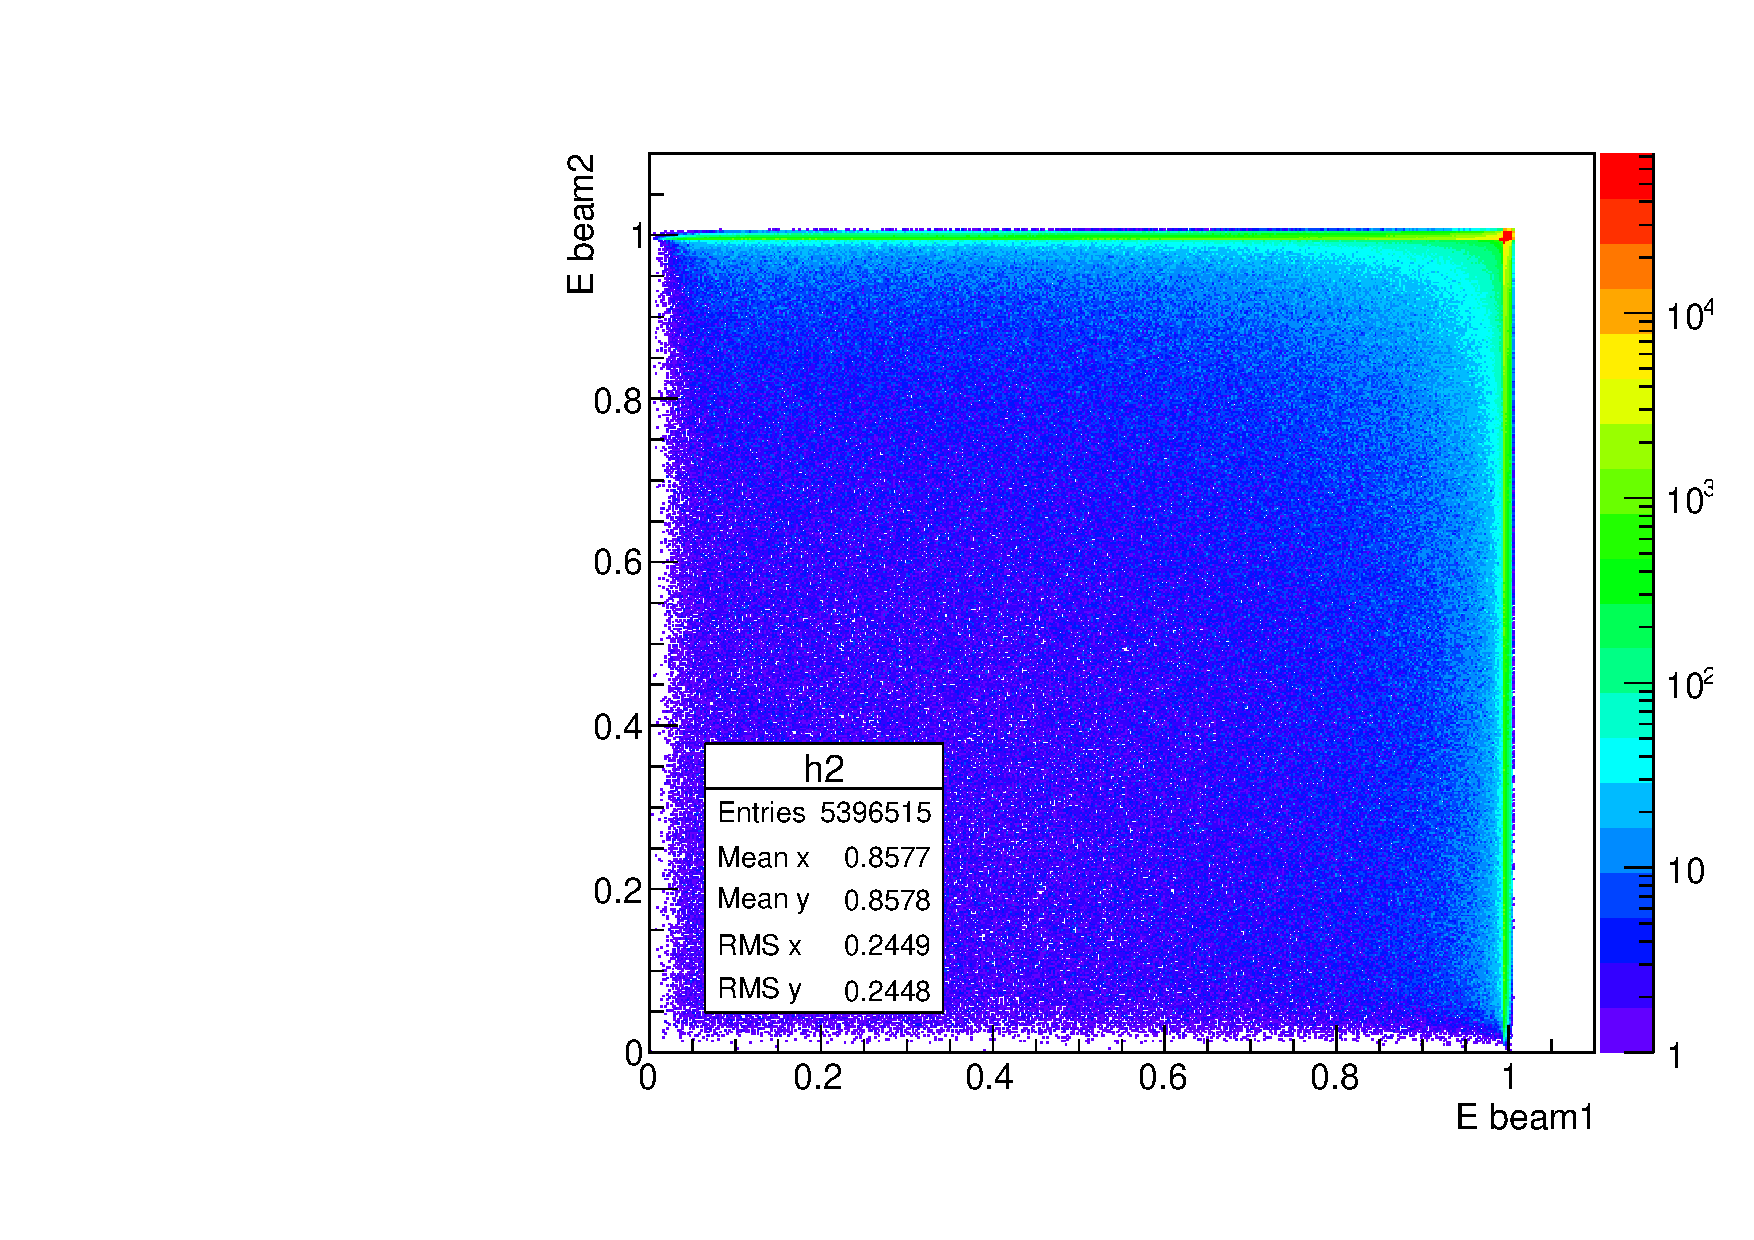
\includegraphics[width=4cm]{E1_E2_spread_strahlung.pdf}
\end{center}
\begin{itemize}
\item need a \alert{model}, based on assumptions and existing Monte
Carlo samples
\item need a framework/procedure for parameter estimation
\end{itemize}

Why the need for a model? Why not use directly Guinea Pig?
\begin{itemize}
  \item Because of the very large number of parameters in GP, input particle
  distributions, etc.
\end{itemize}
\end{frame}

\section{Fit Methods}
\begin{frame}
\frametitle{Fit methods}
Parametrize beam energies and their \alert{correlations} using a model which
gives a set of \alert{parameters $[p]$} to estimate. \\
~\\
Central point of the method: compare histograms (MC vs Data) using $\chi^2$. \\
~\\
For the fit itself, 2 methods:
\begin{itemize}
  \item Brute force (Backup)
  \item Reweighting fit
\end{itemize}
~\\
Relies on existing \alert{Data} (MC at this level) set: here Guinea Pig sample
with CLIC 3TeV nominal settings.\\

\end{frame}


\begin{frame}
\frametitle{Reweighting fit}
\begin{itemize}
  \item A \alert{distribution} of an observable $=$ \alert{``probability''} for
  an event to happen with a given observable value. Observable can be e.g.
  $\{E1,E2\}$ for a given event%, in fact 1 event
  %$=\{E1,E2,\theta_1,\theta_2,E_{ECAL1},E_{ECAL2}\}$)
  \item If said distribution is built from a set of parameters' values
  $[p]$, then probabilities can be computed from that set
  \item Changing $[p]\to [p]'\Rightarrow$ change of the probabilities. This
  change is accounted by the ratio $\frac{P(\{E1,E2\},
  [p]')}{P(\{E1,E2\},[p])}$. This weight is applied individually to every
  event.
  %\item Bhabha events are not only represented by $\{EB1,EB2\}$ but by
  %$\{EB1,EB2,\theta_1,\theta_2,E_{ECAL1},E_{ECAL2},etc.\}$ where the
  %$\{\theta_1,\theta_2,E_{ECAL1},E_{ECAL2},etc.\}$ set are reconstructed
  %(measured) observables
\end{itemize}
Same principle applies when looking at reconstructible obervables (Bhabha
events, see later)
%Can also work with generator level data only.
\end{frame}

\begin{frame}
\frametitle{Reweighting fit}\label{slide:reweightingfit}
%Shown in fig.~\ref{fig:second}
%begin{figure}[h]
\begin{tikzpicture}[scale=.8,auto, remember picture]
\matrix [column sep=5mm,row sep=4mm,ampersand replacement=\&]{
%row1
\uncover<1>{\node [autoblock] (start) {\scriptsize Start};} \& 
~ \& 
~ \&
~ \\
%row2
\uncover<2->{\node [block, color=blue] (gen) {\scriptsize Generate Event with $[p]_0$: $E1$, $E2$, $P(E1,E2;[p]_0)$};} \&
\uncover<3-5>{\node [autoblock, node distance=2.7cm] (bhwide) {\scriptsize BHWide};} \&
\uncover<4-5>{\node [autoblock, node distance=2.5cm] (sim) {\scriptsize Simulation};} \&
\uncover<5-21>{\node [autoblock, node distance=2.7cm] (rec) {\scriptsize
Reconstruction};} \\
%row3
\uncover<6->{\node [block, color=magenta] (minim) {\scriptsize Minimizer: $[p]_N \rightarrow [p]_{N+1}$};} \&
\uncover<7-13,15->{\node [block, text width=2.2cm, node distance=2.7cm] (compute) {\scriptsize Compute $P(E1,E2;[p]_{N+1})$ for all events};} \&
\uncover<8-13,16->{\node [autoblock, node distance=2.8cm] (weight) {\scriptsize $w = \frac{P(E1,E2;[p]_{N+1})}{P(E1,E2;[p]_{0})}$};} \&
\uncover<9-13,17->{\node [block, node distance=2.7cm] (weightrec) {\scriptsize Weight every event with its weight $w$};} \\
%row4
~ \& 
~ \& 
\uncover<11-13,19->{\node [decision, color=violet] (match) {\scriptsize
Minimum?};} \& \uncover<10-13,18->{\node [block, color=red] (compare) {\scriptsize Compare with data: $\chi^2$};}\\
%row5
~ \& 
~ \& 
\uncover<12-13,20->{\node [autoblock] (done) {\scriptsize Done!};} \& 
~ \\
};
\begin{scope}
\uncover<1>{\path [line] (start) -- (gen);}
\uncover<3-5>{\path [line] (gen) -- (bhwide);}
\uncover<4-5>{\path [line] (bhwide) -- (sim);}
\uncover<5>{\path [line] (sim) -- (rec);}
\uncover<6>{\path [line] (gen) -- (minim);}
\uncover<7-13,15->{\path [line] (minim) -- (compute);}
\uncover<8-13,16->{\path [line] (compute) -- (weight);}
\uncover<9-13,17->{\path [line] (weight) -- (weightrec);}
\uncover<10-13,18->{\path [line] (weightrec) -- (compare);}
\uncover<11-13,19->{\path [line] (compare) -- (match);}
\uncover<12-13,20->{\path [line] (match) -- node [near start] {\scriptsize yes} (done);}
\uncover<13,21->{\path [line] (match) -| node [very near start] {\scriptsize no} (minim);}
\uncover<9-13,17-21>{\path [dline] (rec) -- node [midway] {\scriptsize use}
(weightrec); } 
\uncover<22>{\path [dline] (gen) -| node [near start] {Model level fit}
(weightrec);}
\end{scope}
\end{tikzpicture}
%\end{figure}
\end{frame}

\begin{frame}
\frametitle{Fit timing}
\begin{itemize}
  \item 4\,000 function calls (loop in slide~\ref{slide:reweightingfit}) for the minimization:
  $\sim12$h
  \item 2 weeks for the simulation/reconstruction of 5\,000\,000 events
\end{itemize}
\begin{center}
\alert{That's the way to go!}
\end{center}
\end{frame}

\section{The Model}
\begin{frame}
\frametitle{Understanding the physics}
Building a model:
\begin{itemize}
  \item understanding the beam-beam interactions
  \item accounting for the beam spread
  \item adding the effects of beamstrahlung
\end{itemize}
\end{frame}

\begin{frame}
\frametitle{Particle distribution in a beam}\label{slide:evsz}
\begin{columns}[c]
\column{6cm}
\begin{tikzpicture}[auto]
\node {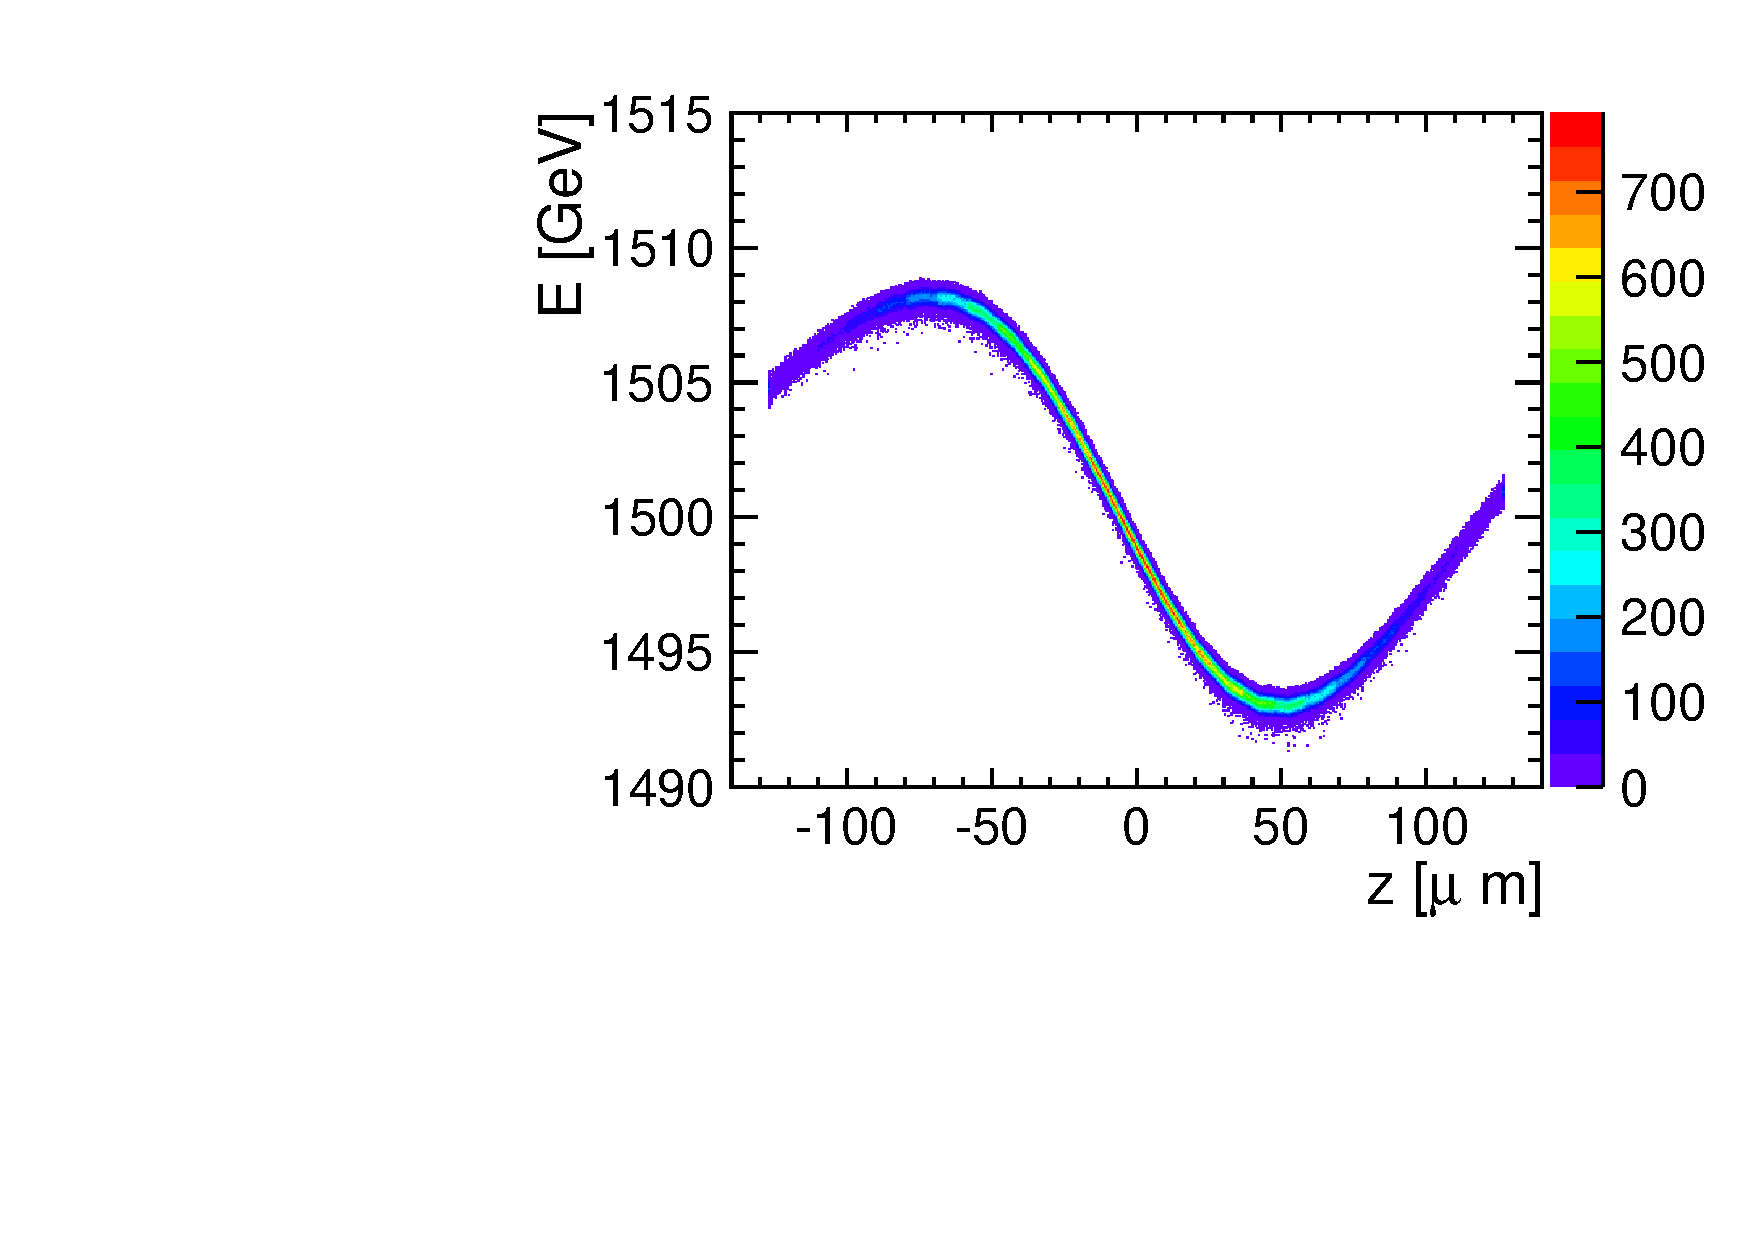
\includegraphics[width=6cm]{E_vs_v_colz_electrons.pdf}};
\draw [->, thick, color=red](2,-2.4) -- node [midway] {beam direction}(-2,-2.4);
\end{tikzpicture}
\column{6cm}
\begin{tikzpicture}
\node (fig) {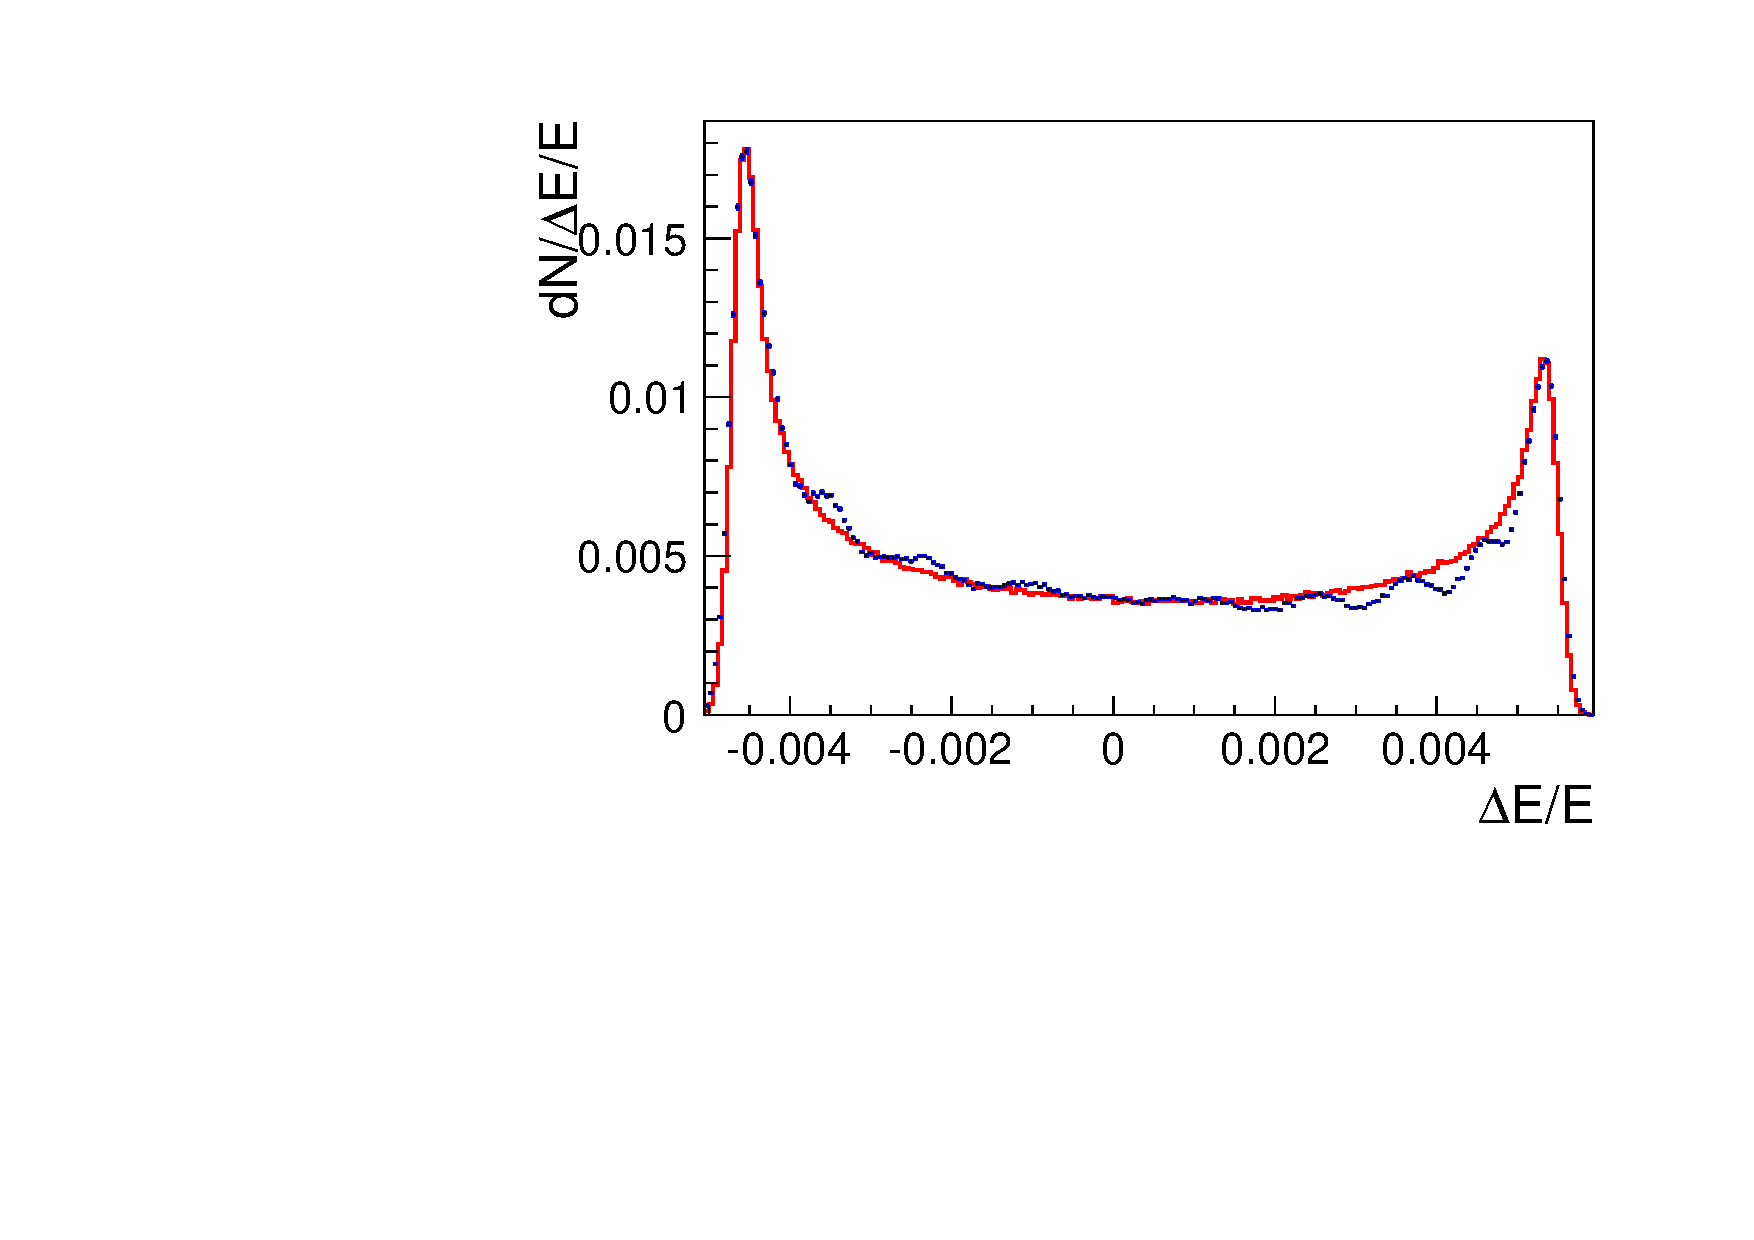
\includegraphics[width=6cm]{MCBeamSpreadFCAL.pdf}};
\node at (0,-2.4) {Projection on E, normalized, fitted};
%\node {Beam energy spread};
\end{tikzpicture}
\end{columns}

Back of the beam has less energy.
\end{frame}

\begin{frame}
\frametitle{Beam energy spread}\label{slide:beamspread}
Guinea pig \alert{with} beam spread and \alert{without} beamstrahlung:\\
\begin{columns}[c]
\column{6cm}
\begin{tikzpicture}
\node {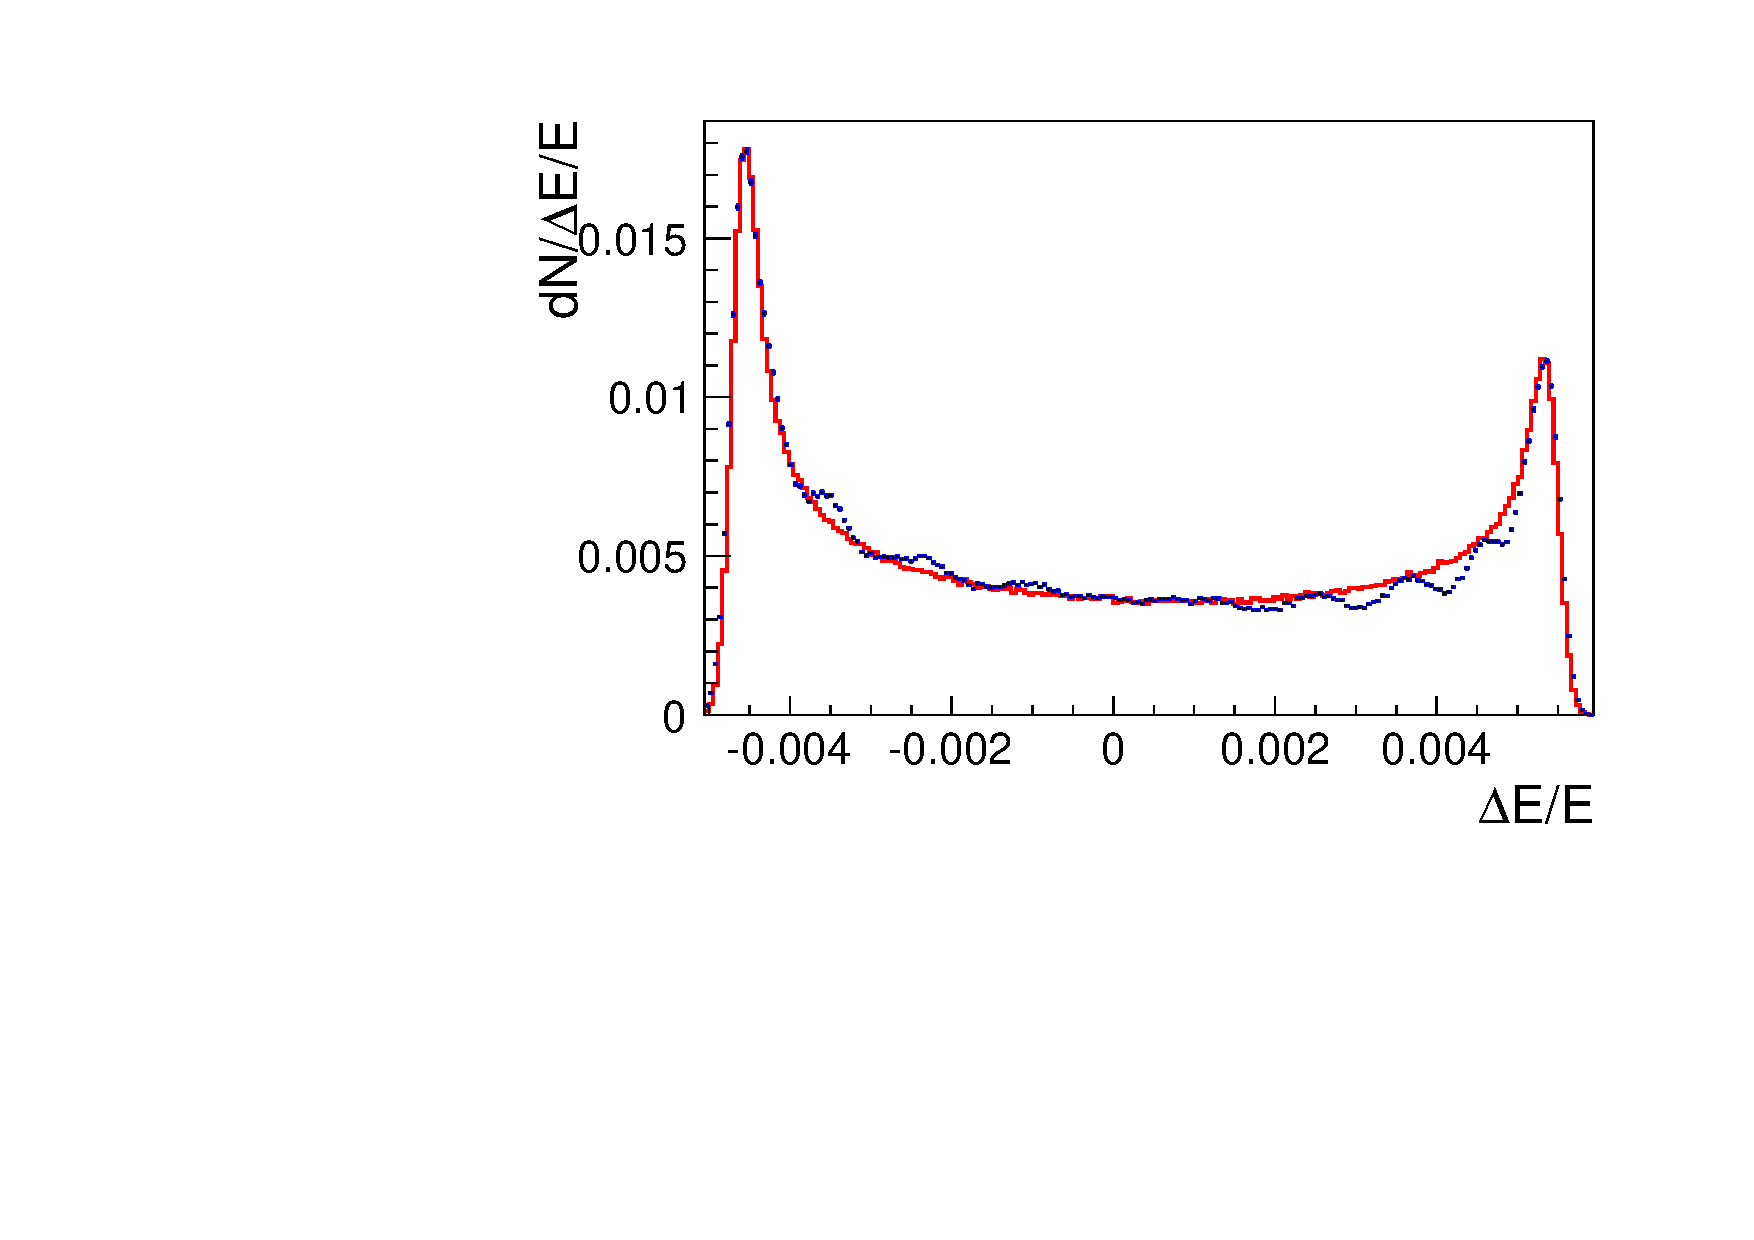
\includegraphics[width=6cm]{MCBeamSpreadFCAL.pdf}};
%\node {Beam energy spread};
\end{tikzpicture}
\column{6cm}
\begin{tikzpicture}
\node {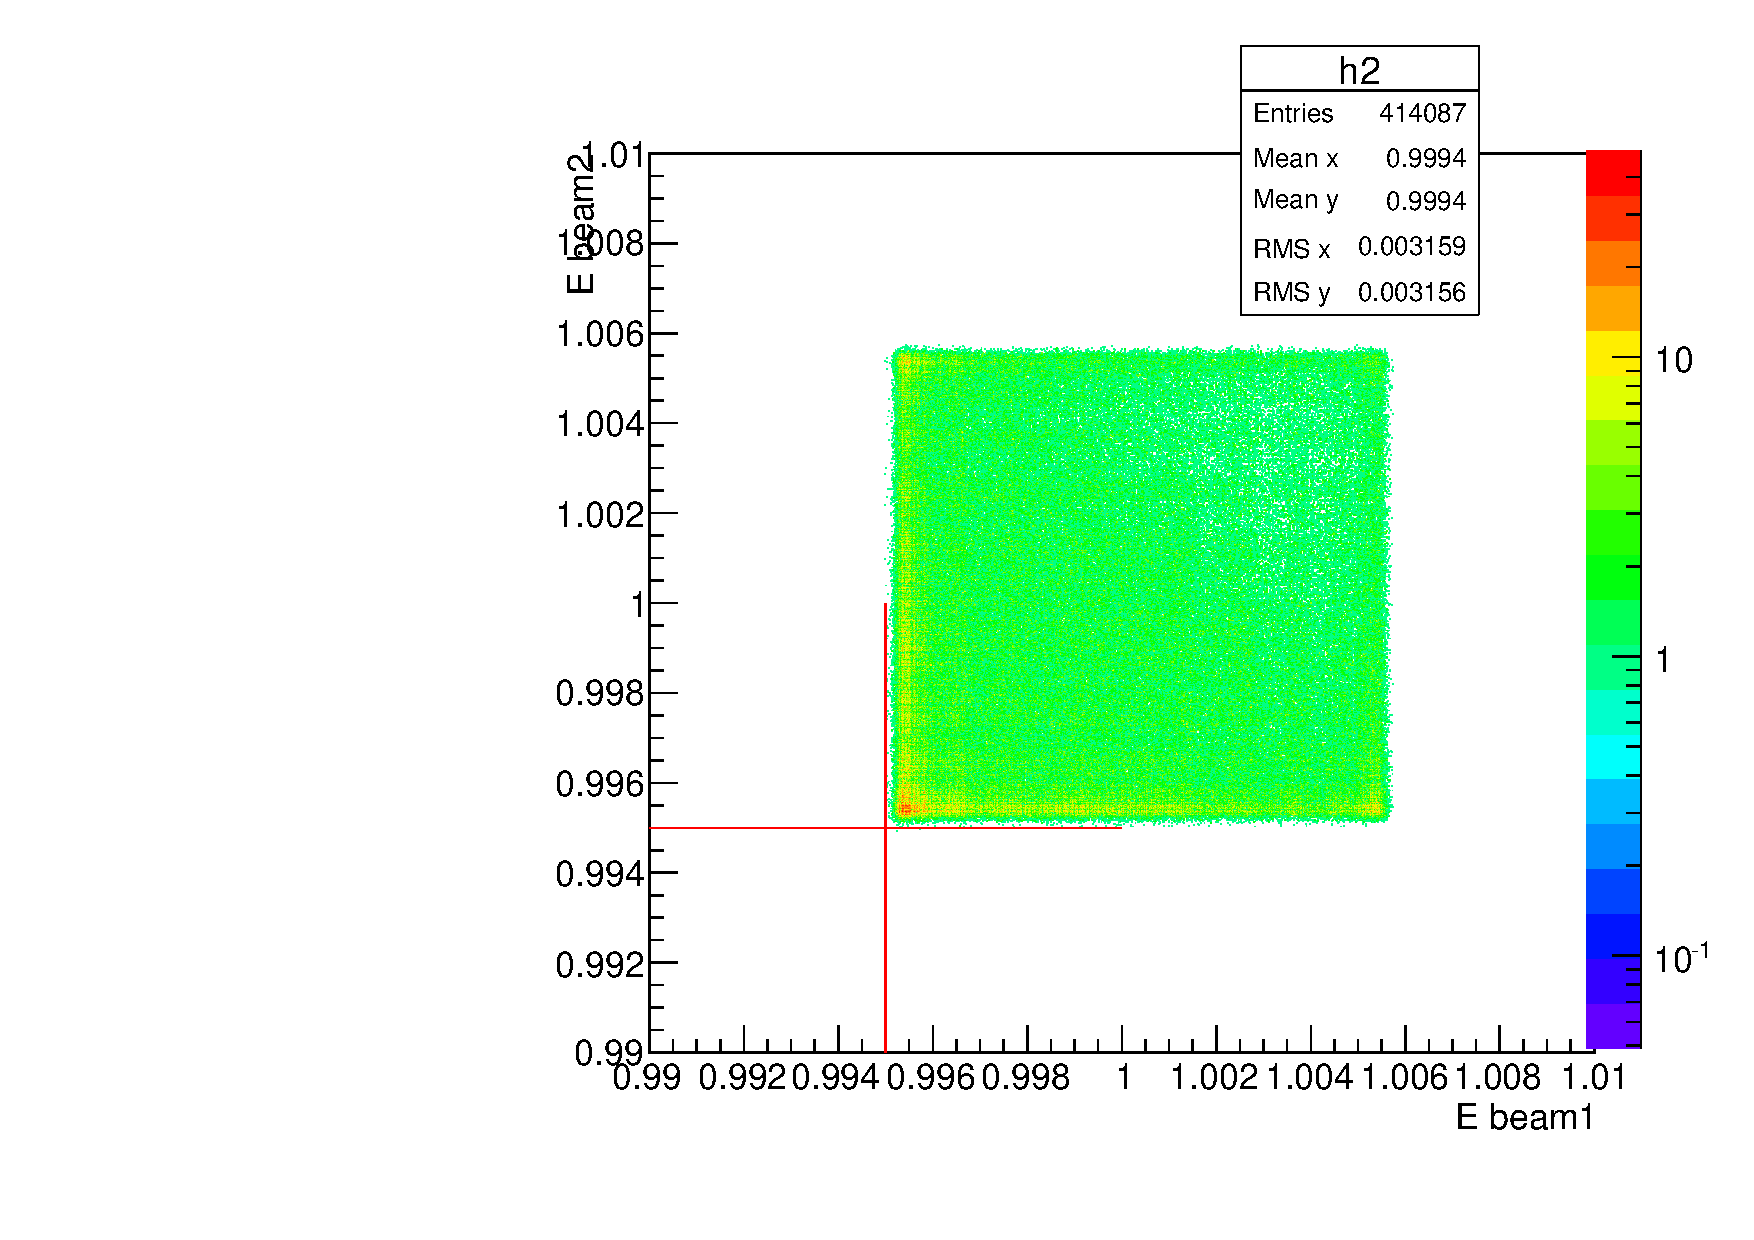
\includegraphics[width=6cm]{E1_E2_spread_nostrahlung.pdf}};
\end{tikzpicture}
\end{columns}

\end{frame}

\begin{frame}
\frametitle{Beamstrahlung effects}\label{slide:beamstrahlung}
Guinea pig \alert{without} beam spread but \alert{with} beamstrahlung:\\
\begin{columns}[c]
\column{6cm}
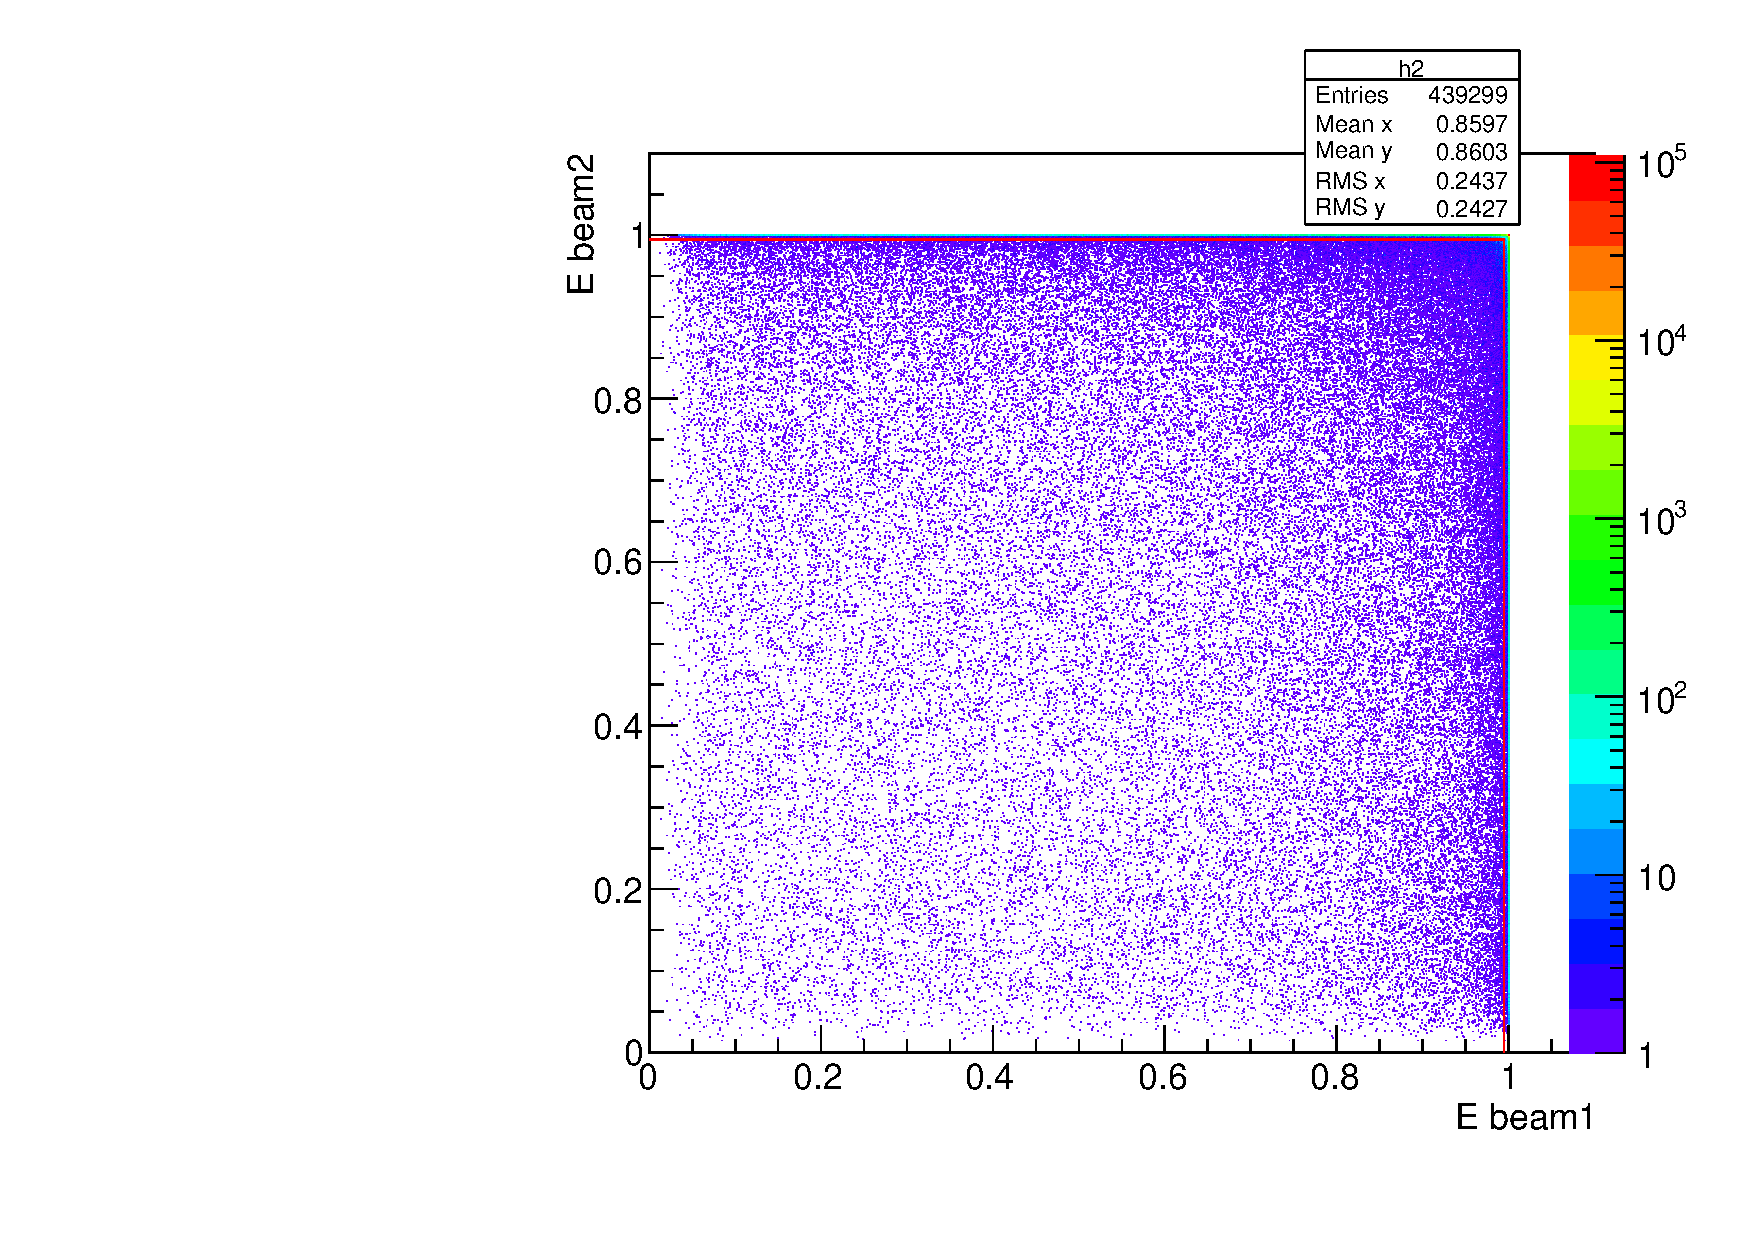
\includegraphics[width=6cm]{E1_E2_nospread_with_strahlung.pdf}
 \column{6cm}
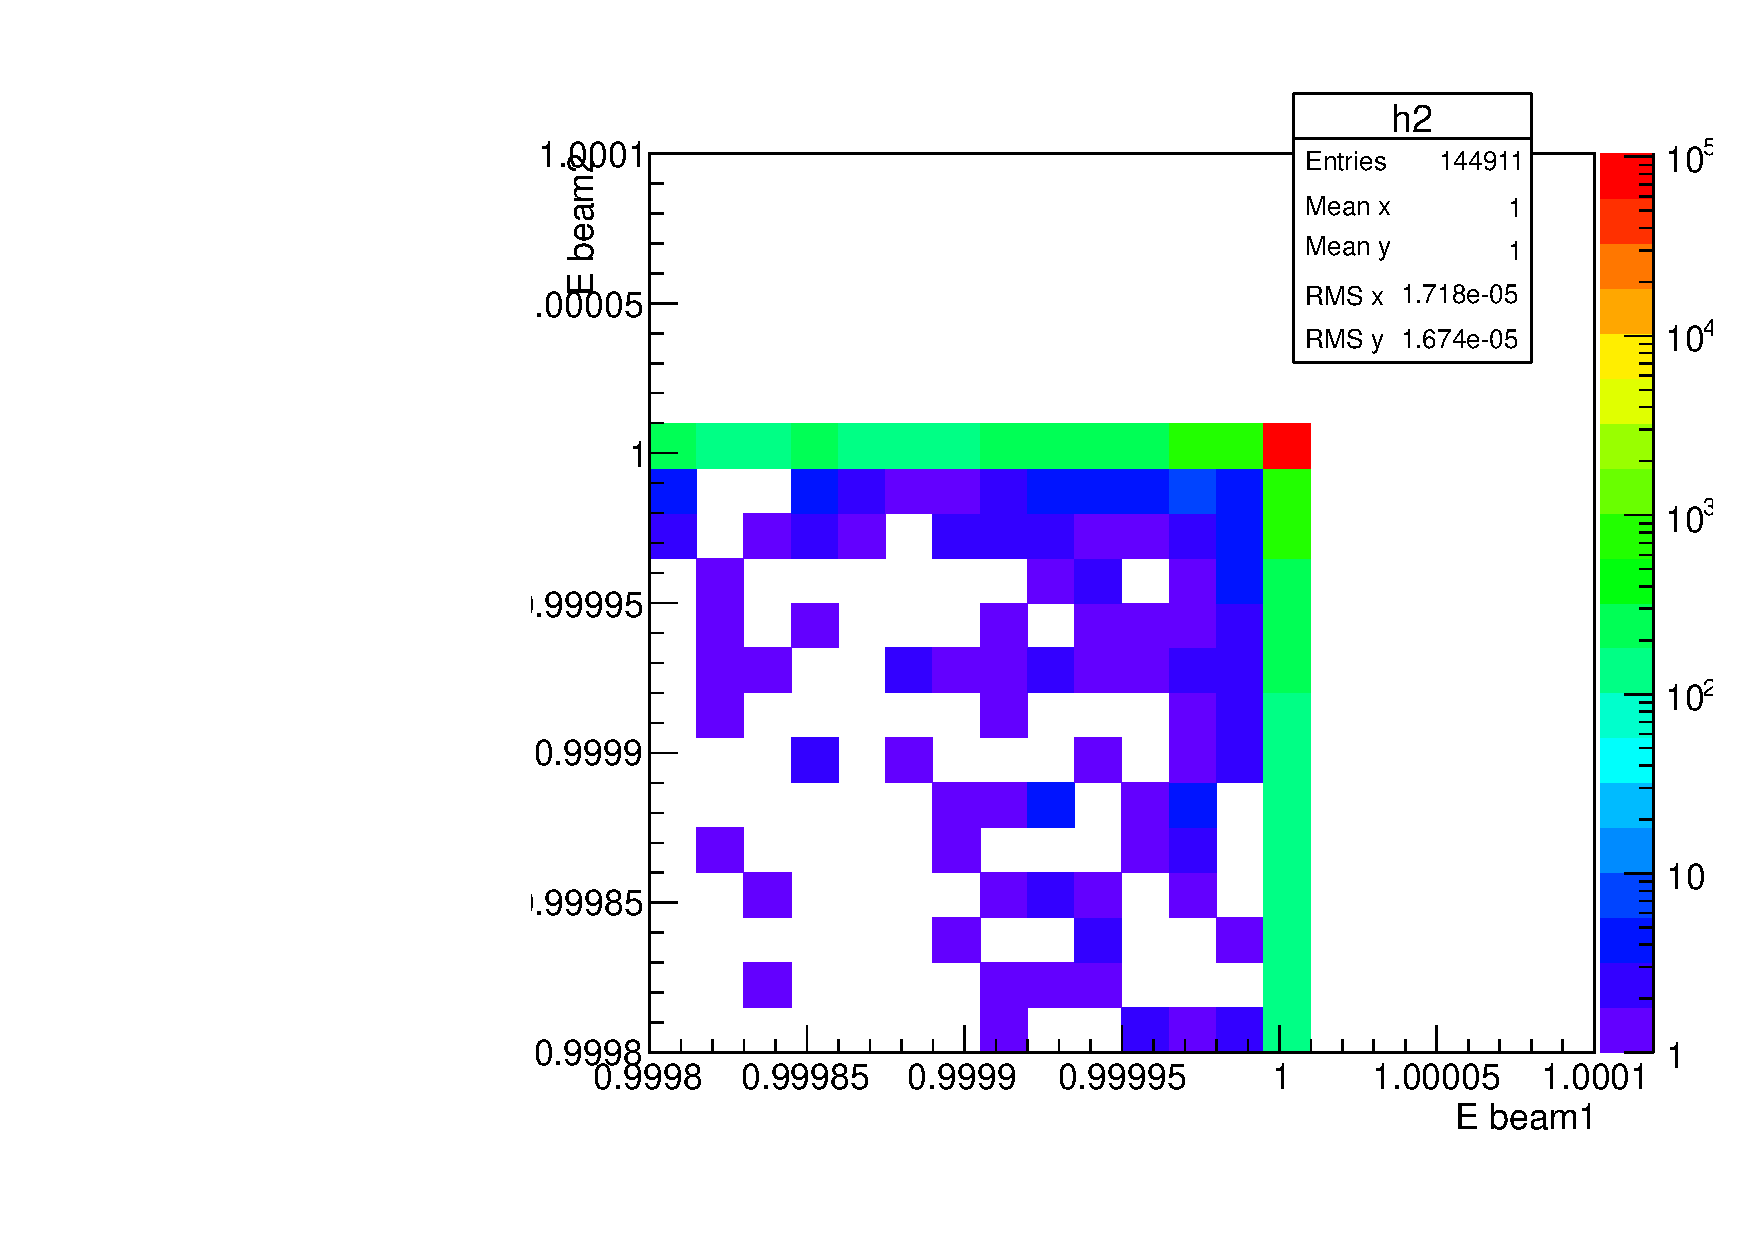
\includegraphics[width=6cm]{E1_E2_nospread_strahlung_zoom.pdf}
\end{columns}
\end{frame}

\begin{frame}
\frametitle{Beam-Beam interactions}
Guinea pig \alert{with} beam spread and \alert{with} beamstrahlung:\\
\begin{columns}[c]
\column{6cm}
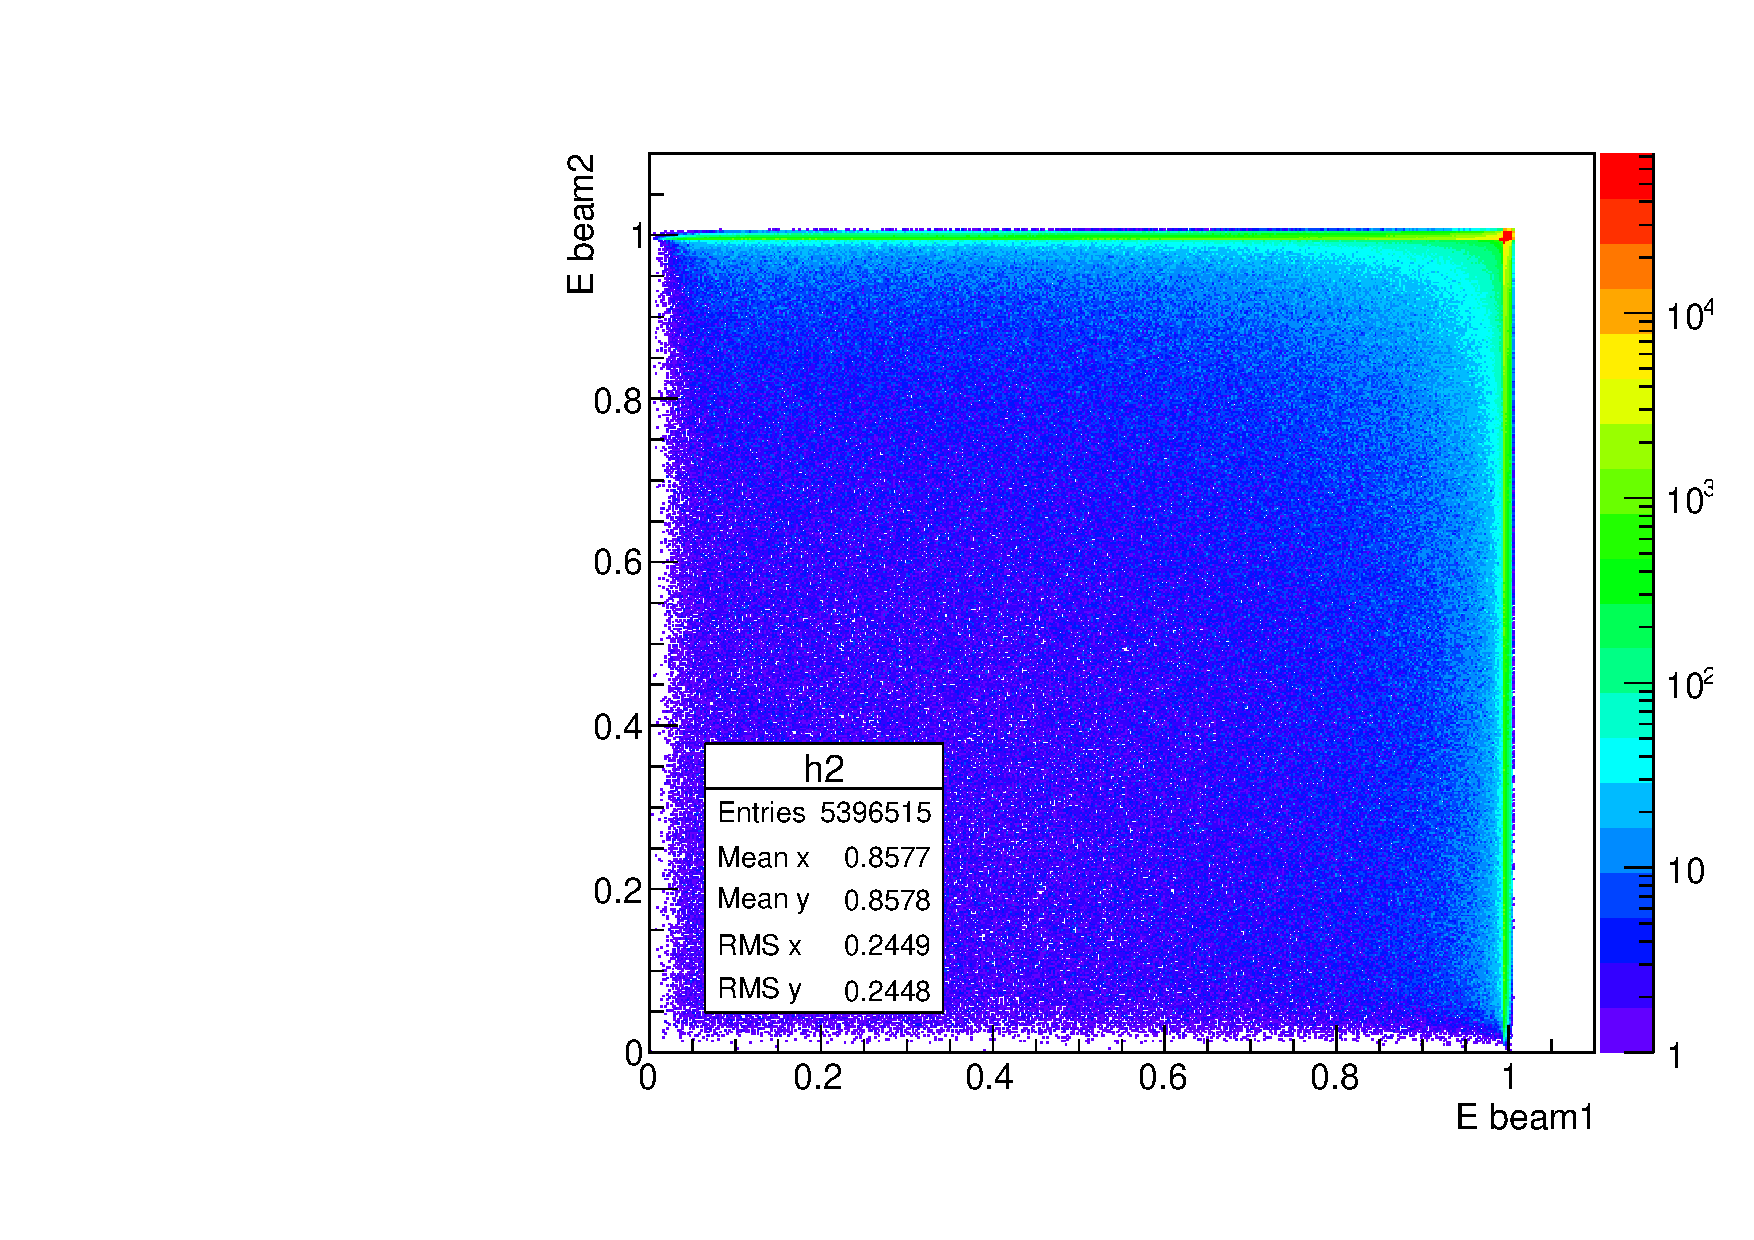
\includegraphics[width=6cm]{E1_E2_spread_strahlung.pdf}
\column{6cm}
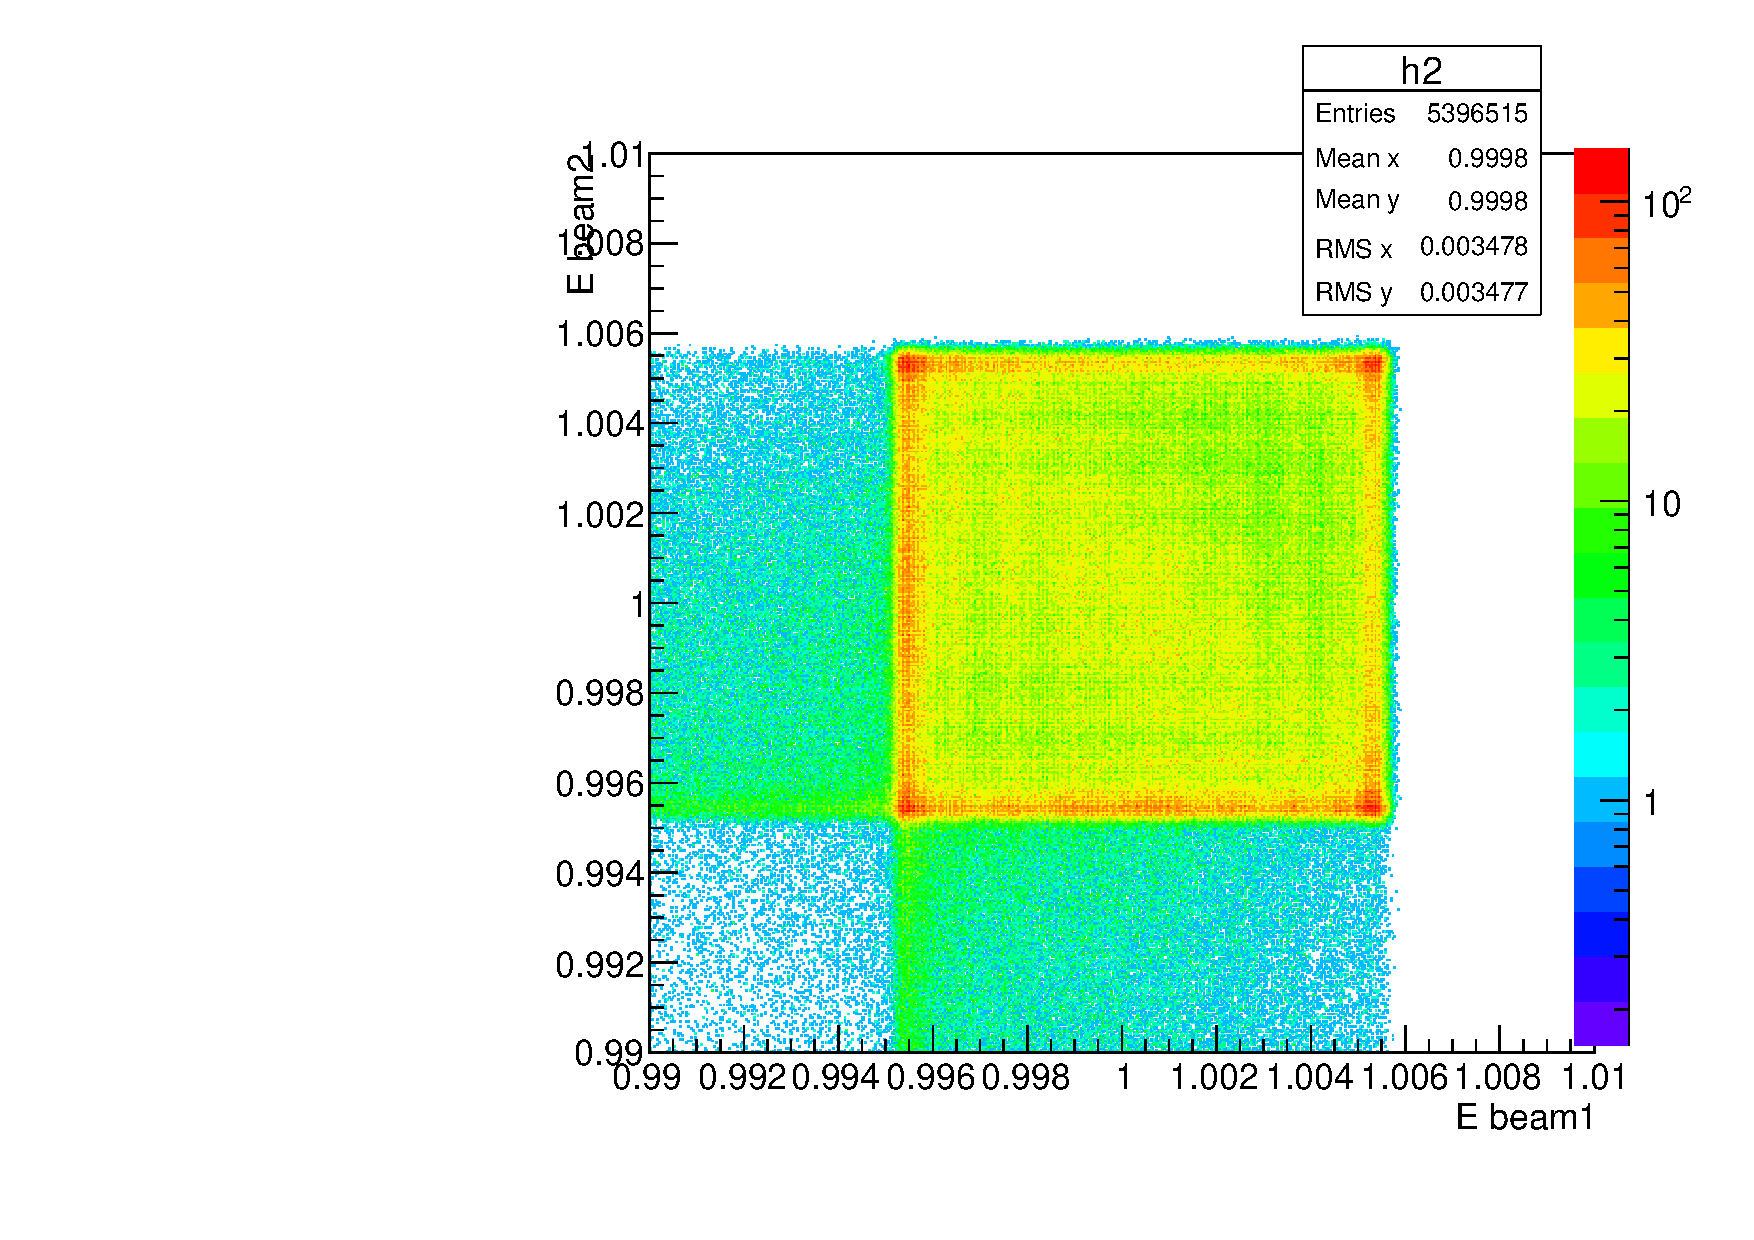
\includegraphics[width=6cm]{E1_E2_spread_strahlung_zoom.pdf}
\end{columns}
\end{frame}

\begin{frame}
\frametitle{Getting a model for the peak}
\begin{center}
\begin{tikzpicture}
\node {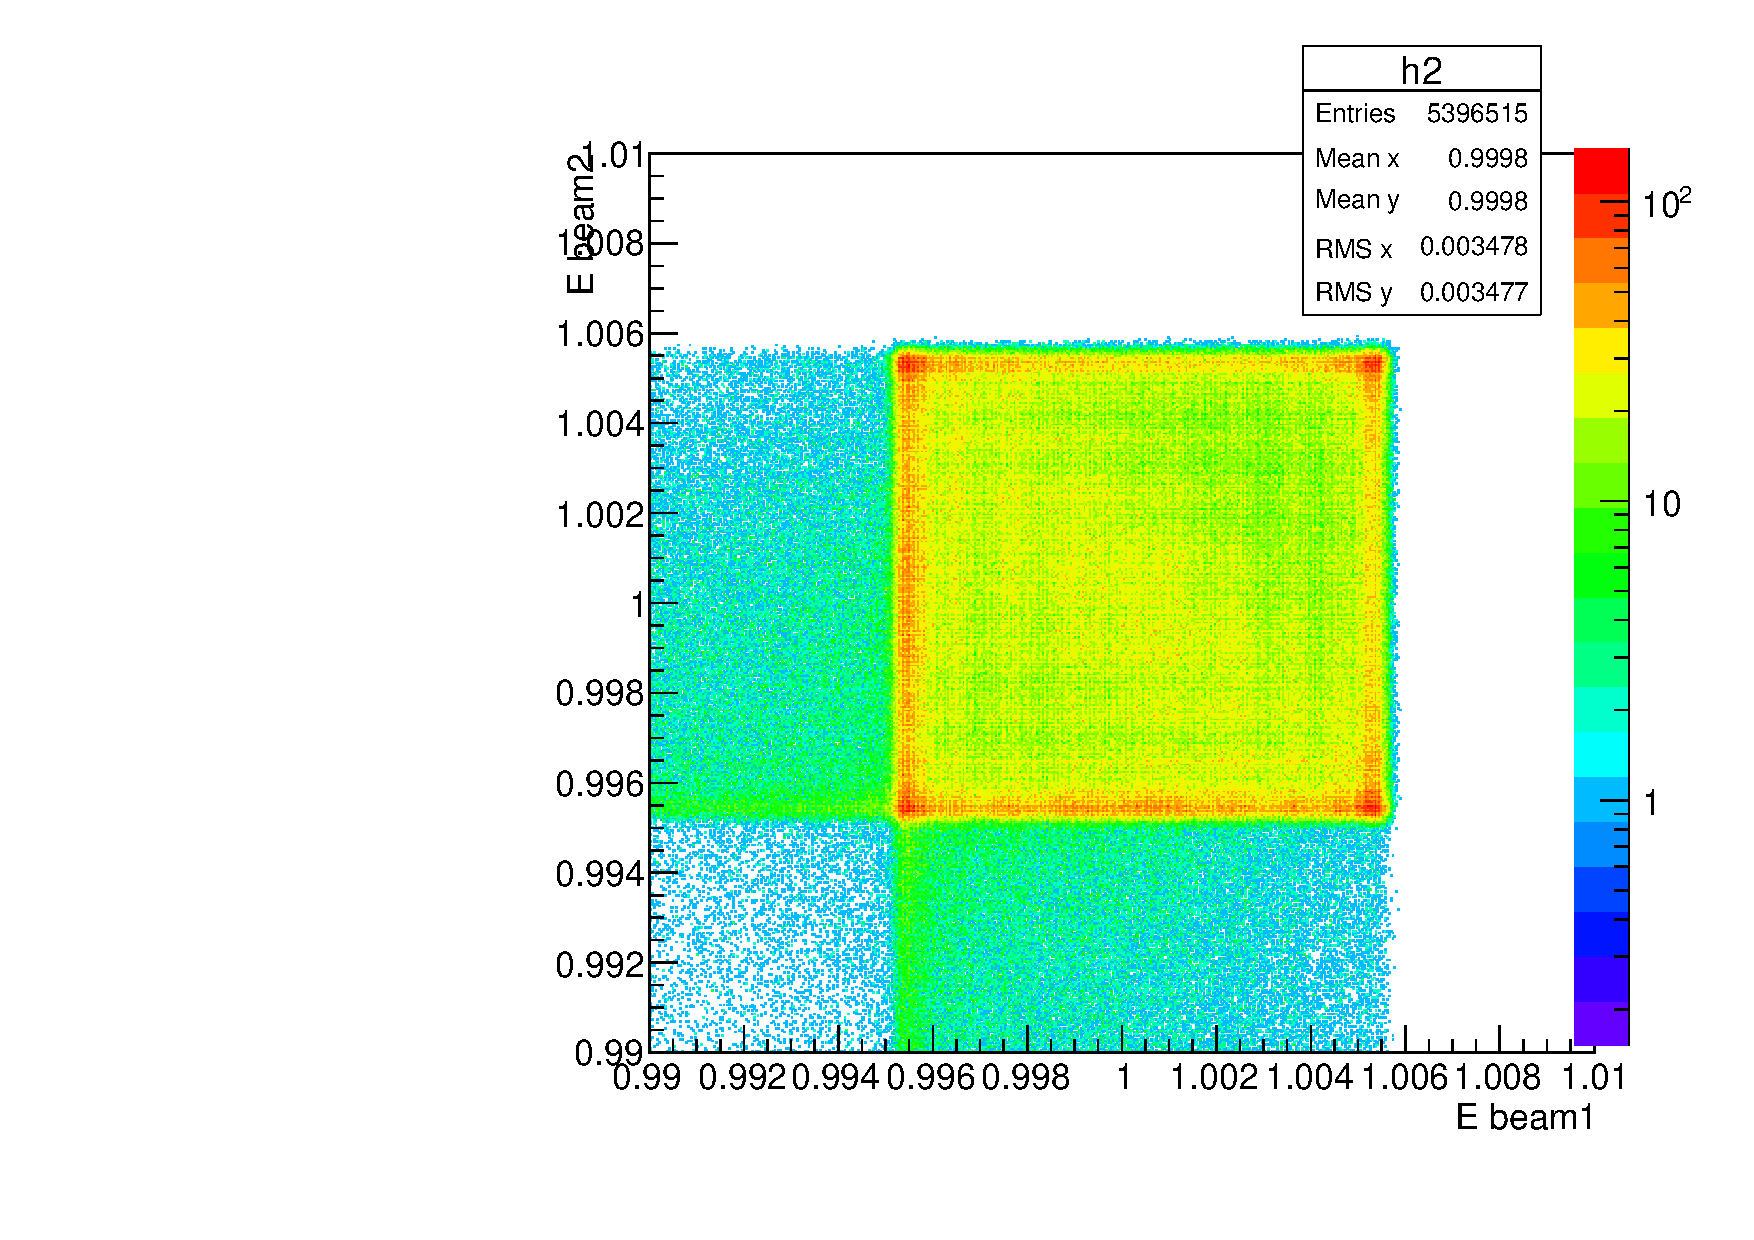
\includegraphics[width=5cm]{E1_E2_spread_strahlung_zoom.pdf}};
\node at (0,0) {peak};
\end{tikzpicture}
\end{center}
Using slide~\ref{slide:beamspread} and slide~\ref{slide:beamstrahlung}:
\begin{itemize}
  \item Use 1 beta distribution for each beam for the ``box''
  (slide~\ref{slide:betadistspreadpeak})
  \item neglect the effect of beamstrahlung: events contributing mostly to the
  peak did not emit beamstrahlung
\end{itemize}
Same range for the beam spread shape for both beams. 
\end{frame}
\begin{frame}
\frametitle{Getting a model for the arms}
\begin{columns}[c]
\column{6cm}
\begin{tikzpicture}
\node {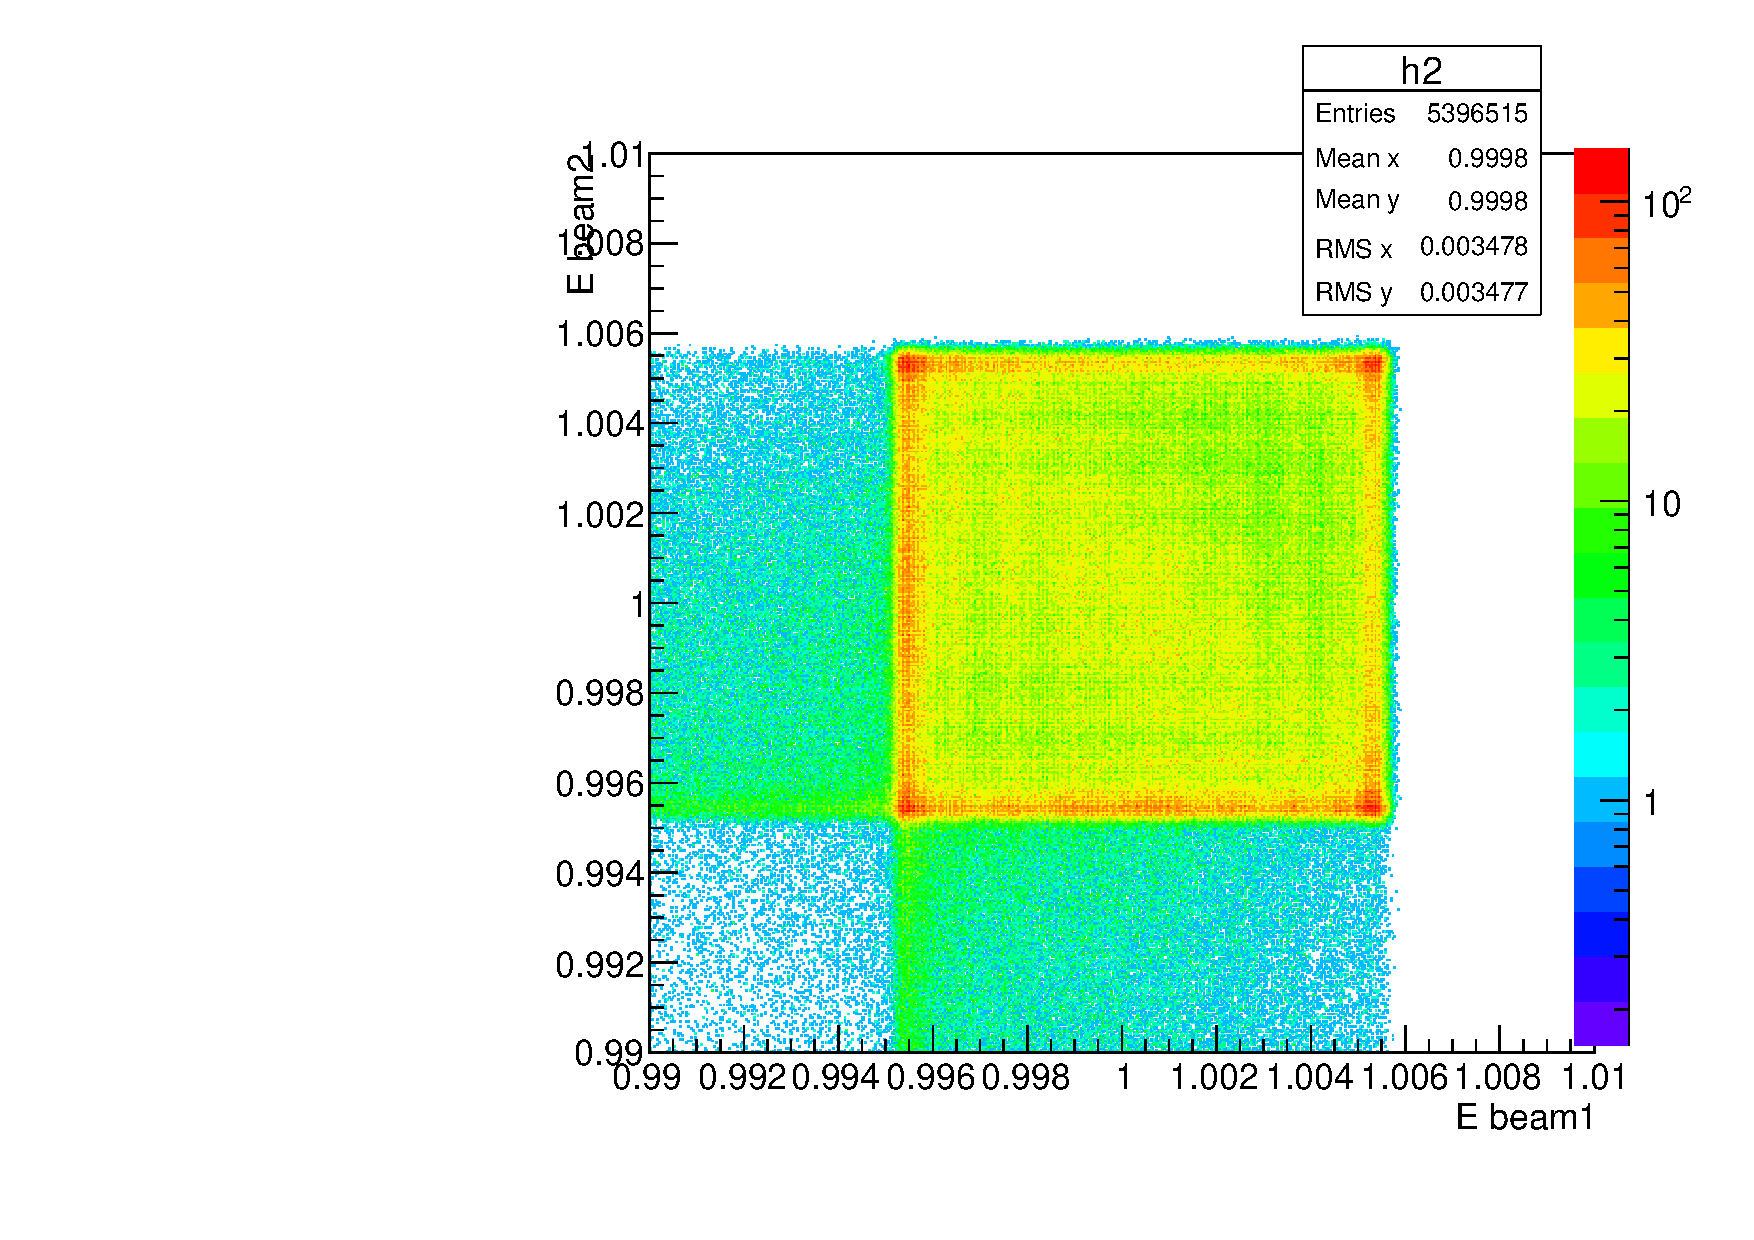
\includegraphics[width=6cm]{E1_E2_spread_strahlung_zoom.pdf}};
%\draw [color=red,thick] (-2.4,1.3) to (-1.2,1.3);
%\draw [color=red,thick] (-2.4,-1.15) to (-1.2,-1.15);
%\draw [color=red,thick] (-1.2,-1.15) to (-1.2,1.3);
\draw [color=red,thick] (-2.4,-1.15) rectangle (-1.2,1.3);
\node at (-1.8,0){arm1};
\draw [color=red,thick] (-1.2,-1.15) rectangle (1.4,-2.3);
\node at (0,-1.5){arm2};
\end{tikzpicture}
\column{6cm}
\begin{center}
Arm 2:\\
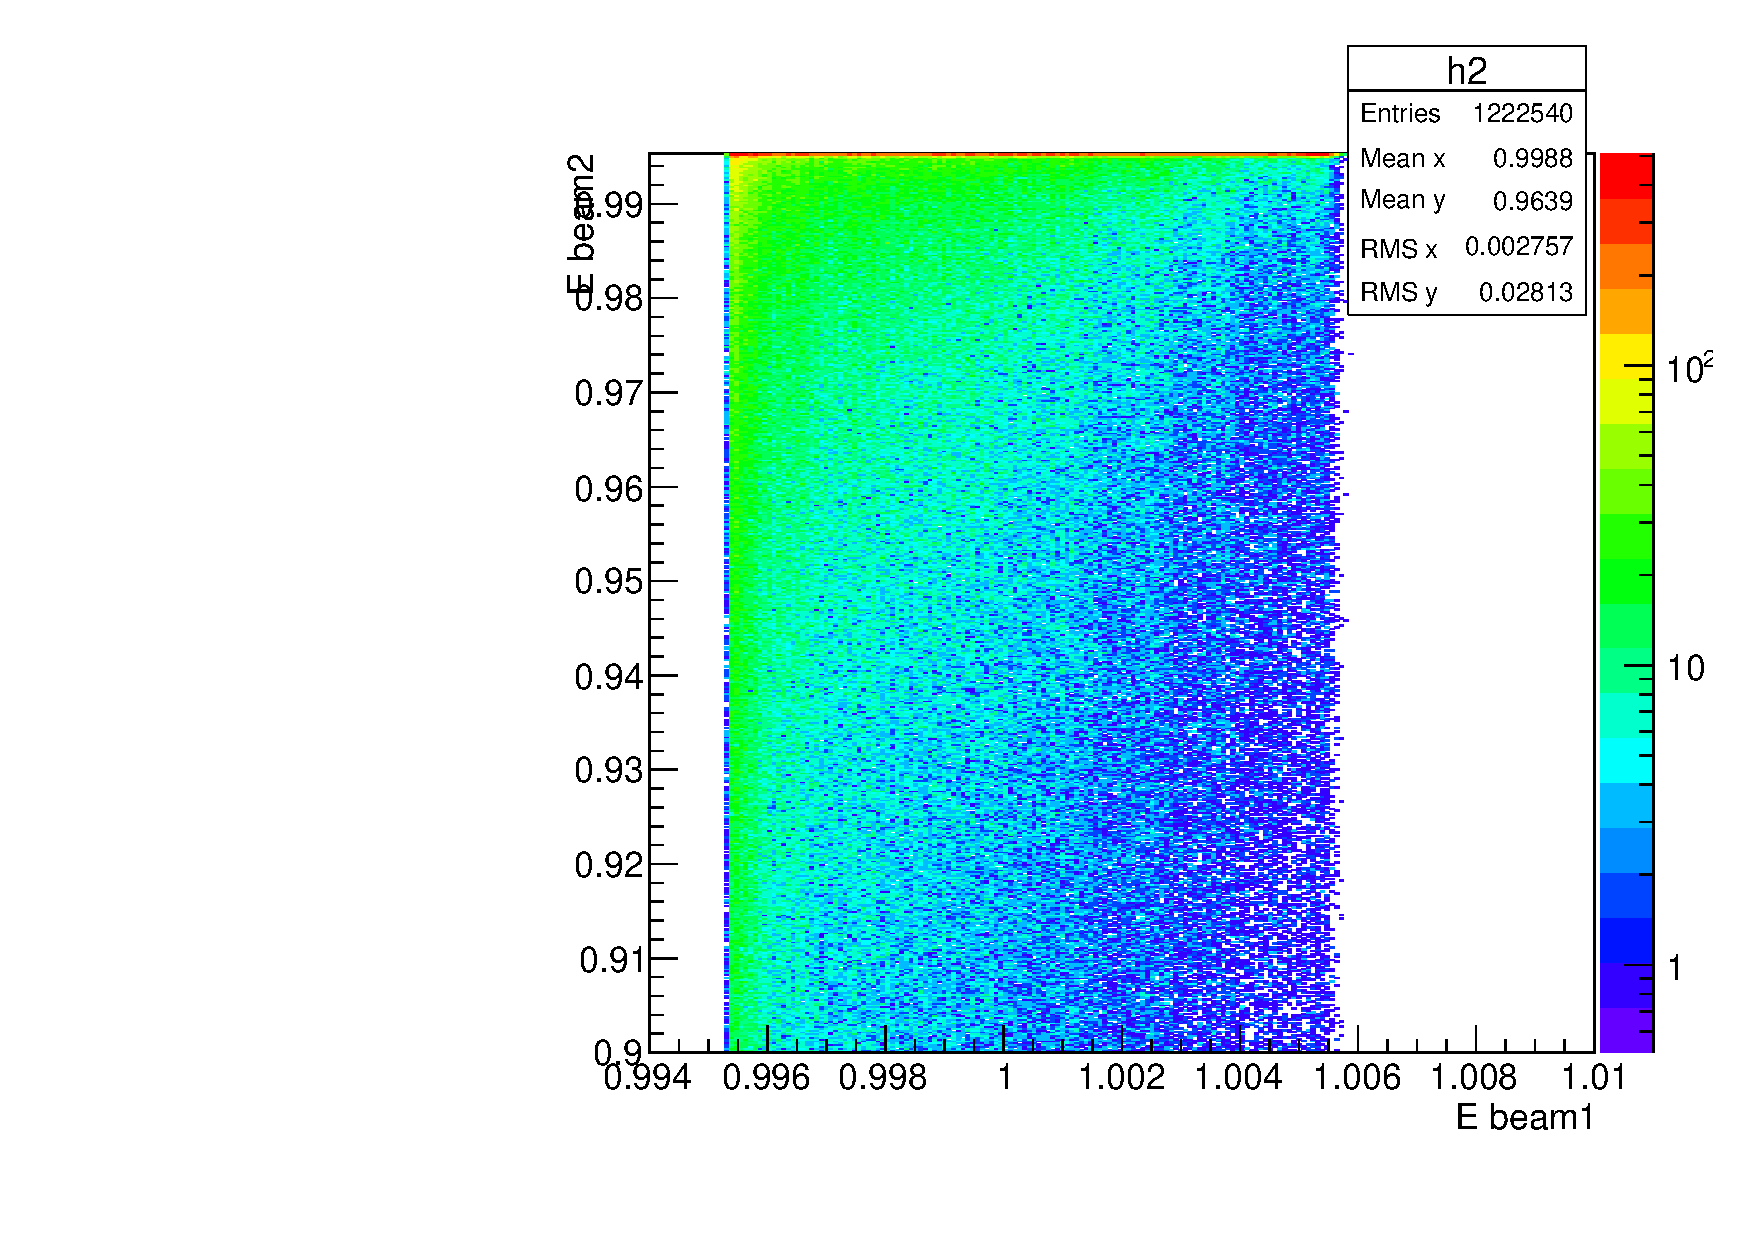
\includegraphics[width=6cm]{Arm2.pdf}
\end{center}
\end{columns}
\end{frame}
\begin{frame}
\frametitle{Getting a model for the arms}
\begin{center}
\begin{tikzpicture}
\node{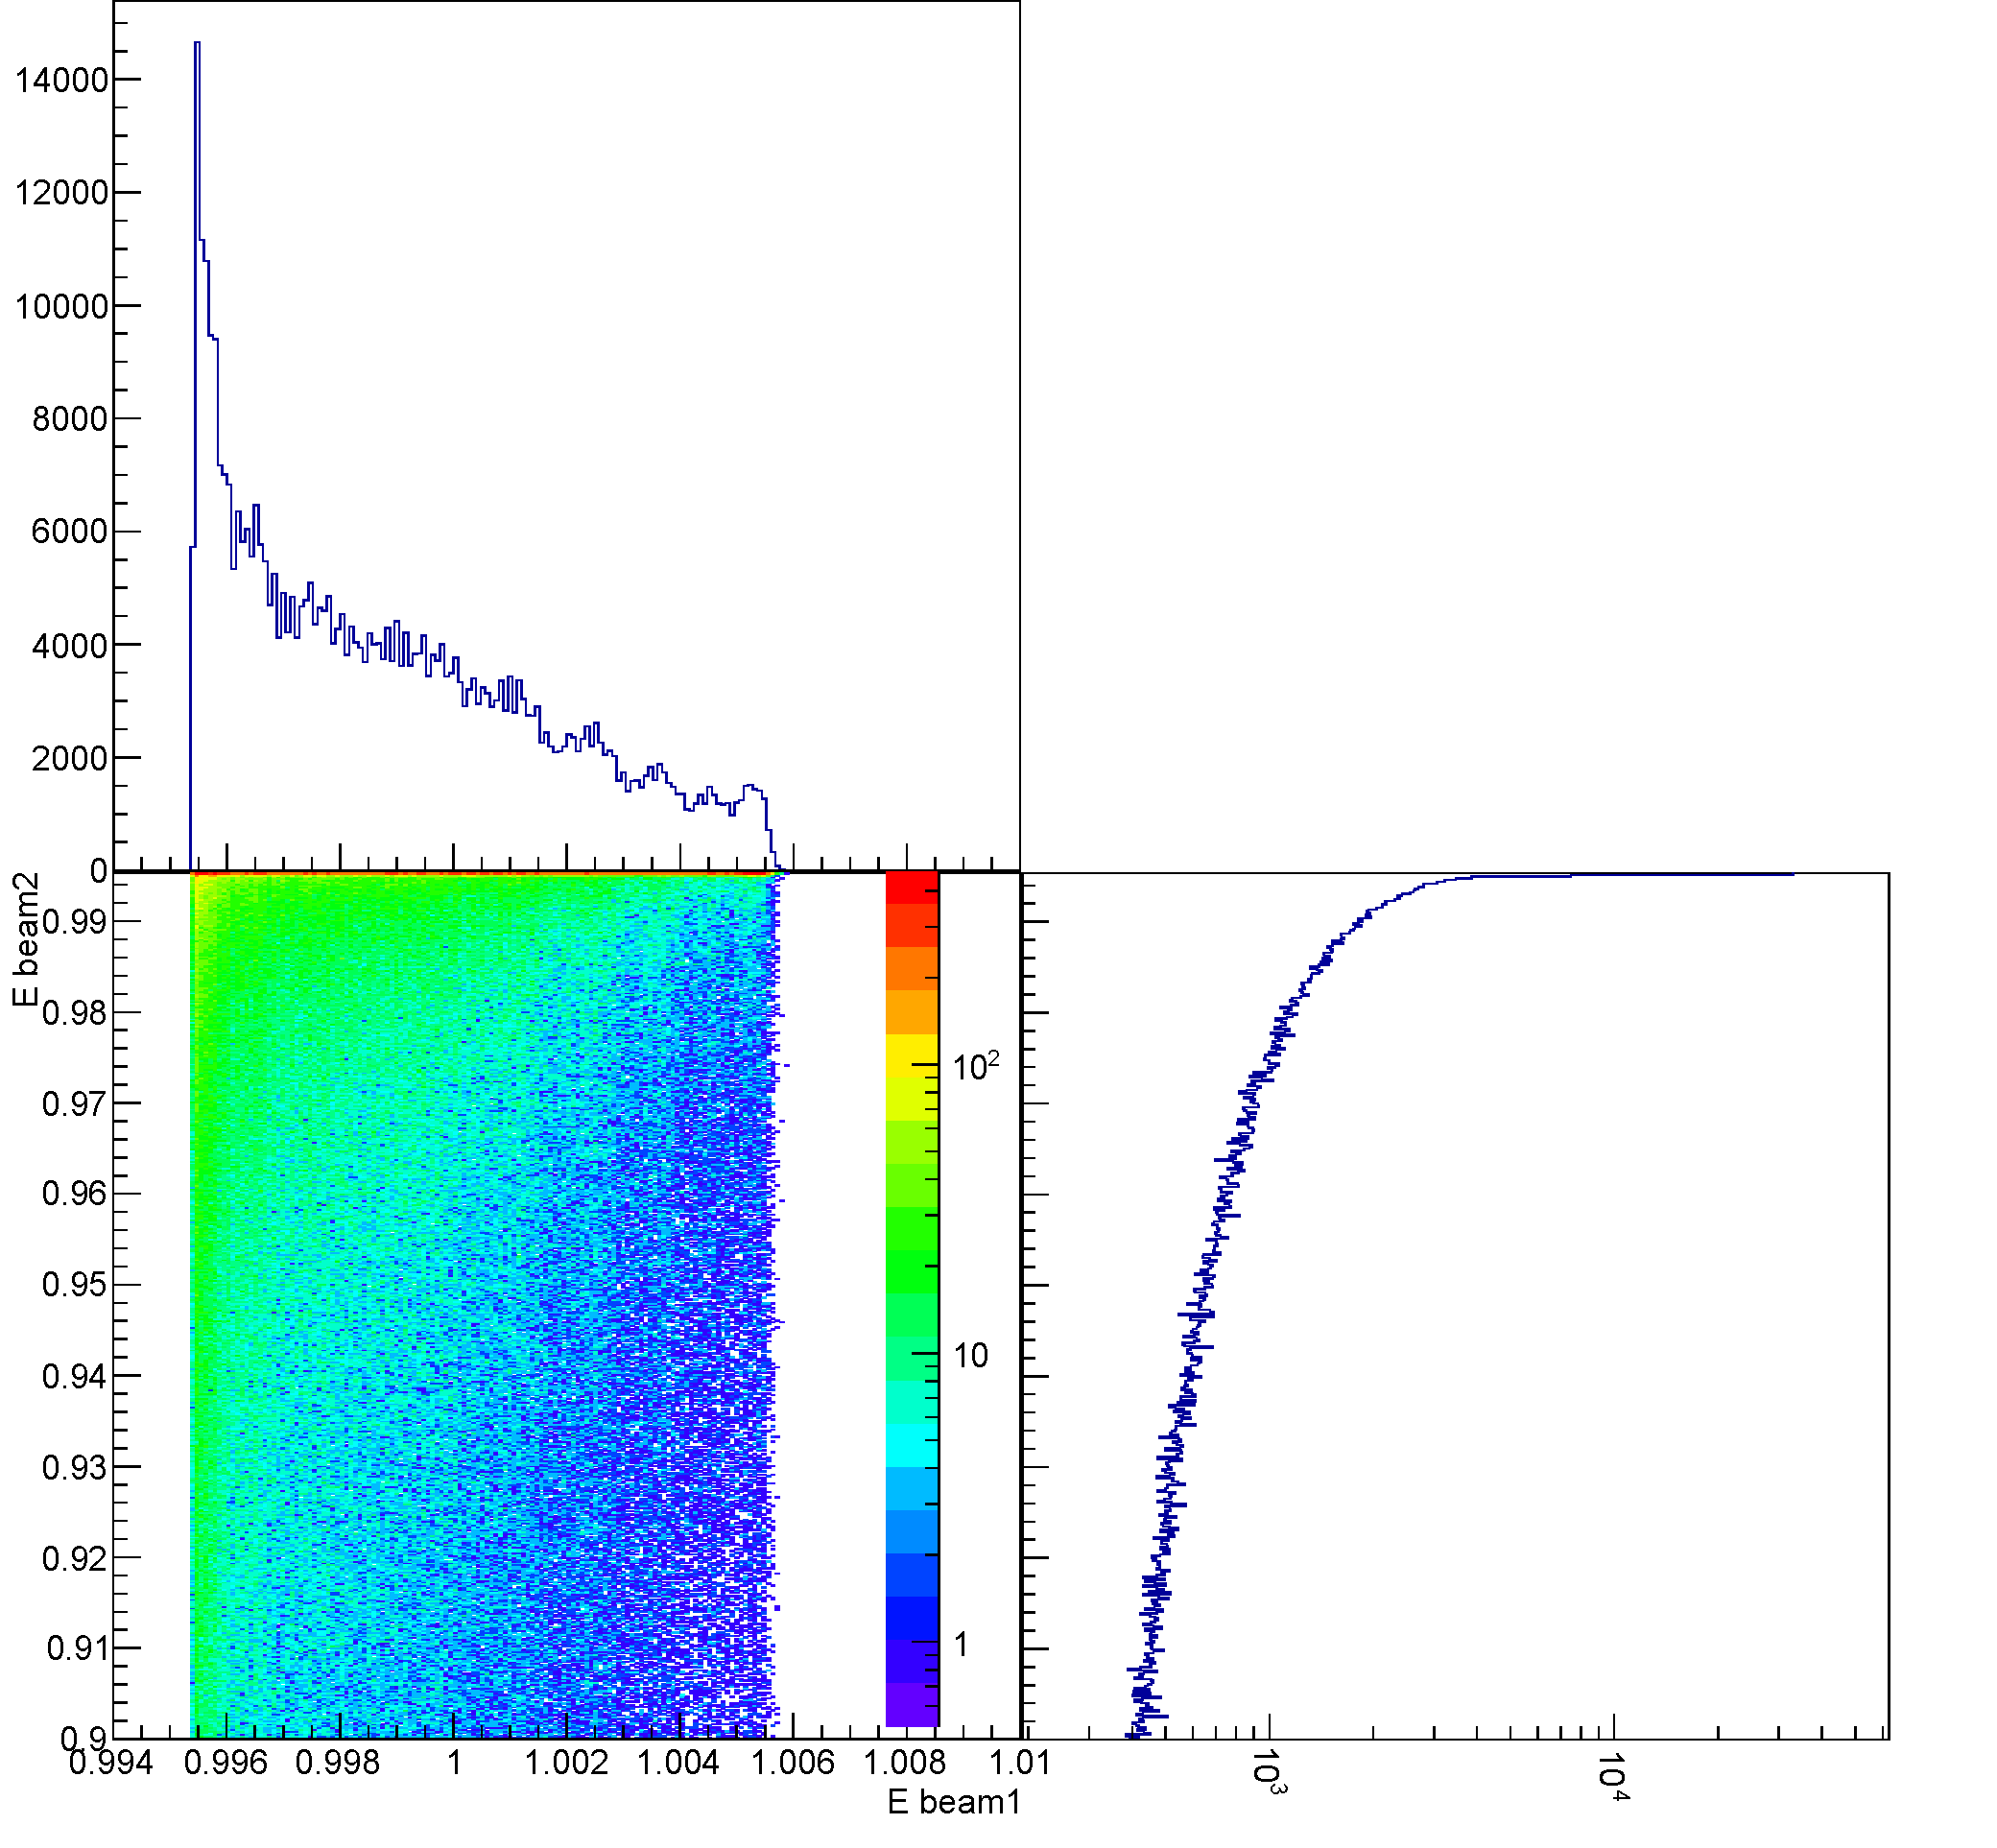
\includegraphics[width=8.5cm]{Arm2_both.pdf}};
\node [scale = 0.7] at (2,3.5) {Projection on E1:};
\node [scale = 0.7] at (3,3) {Similar to the back of the beam spread:};
\node [scale = 0.7] at (3,2.5) {beta distribution, beamstrahlung neglected};
\node [scale = 0.7] at (2,1.5) {Projection on E2:};
\node [scale = 0.7] at (3,1.) {Beamstrahlung only: beta distribution,};
\node [scale = 0.7] at (2,0.5) {beamspread neglected };
\end{tikzpicture}
\end{center}
\end{frame}

\begin{frame}
\frametitle{Getting a model for the body}
\begin{center}
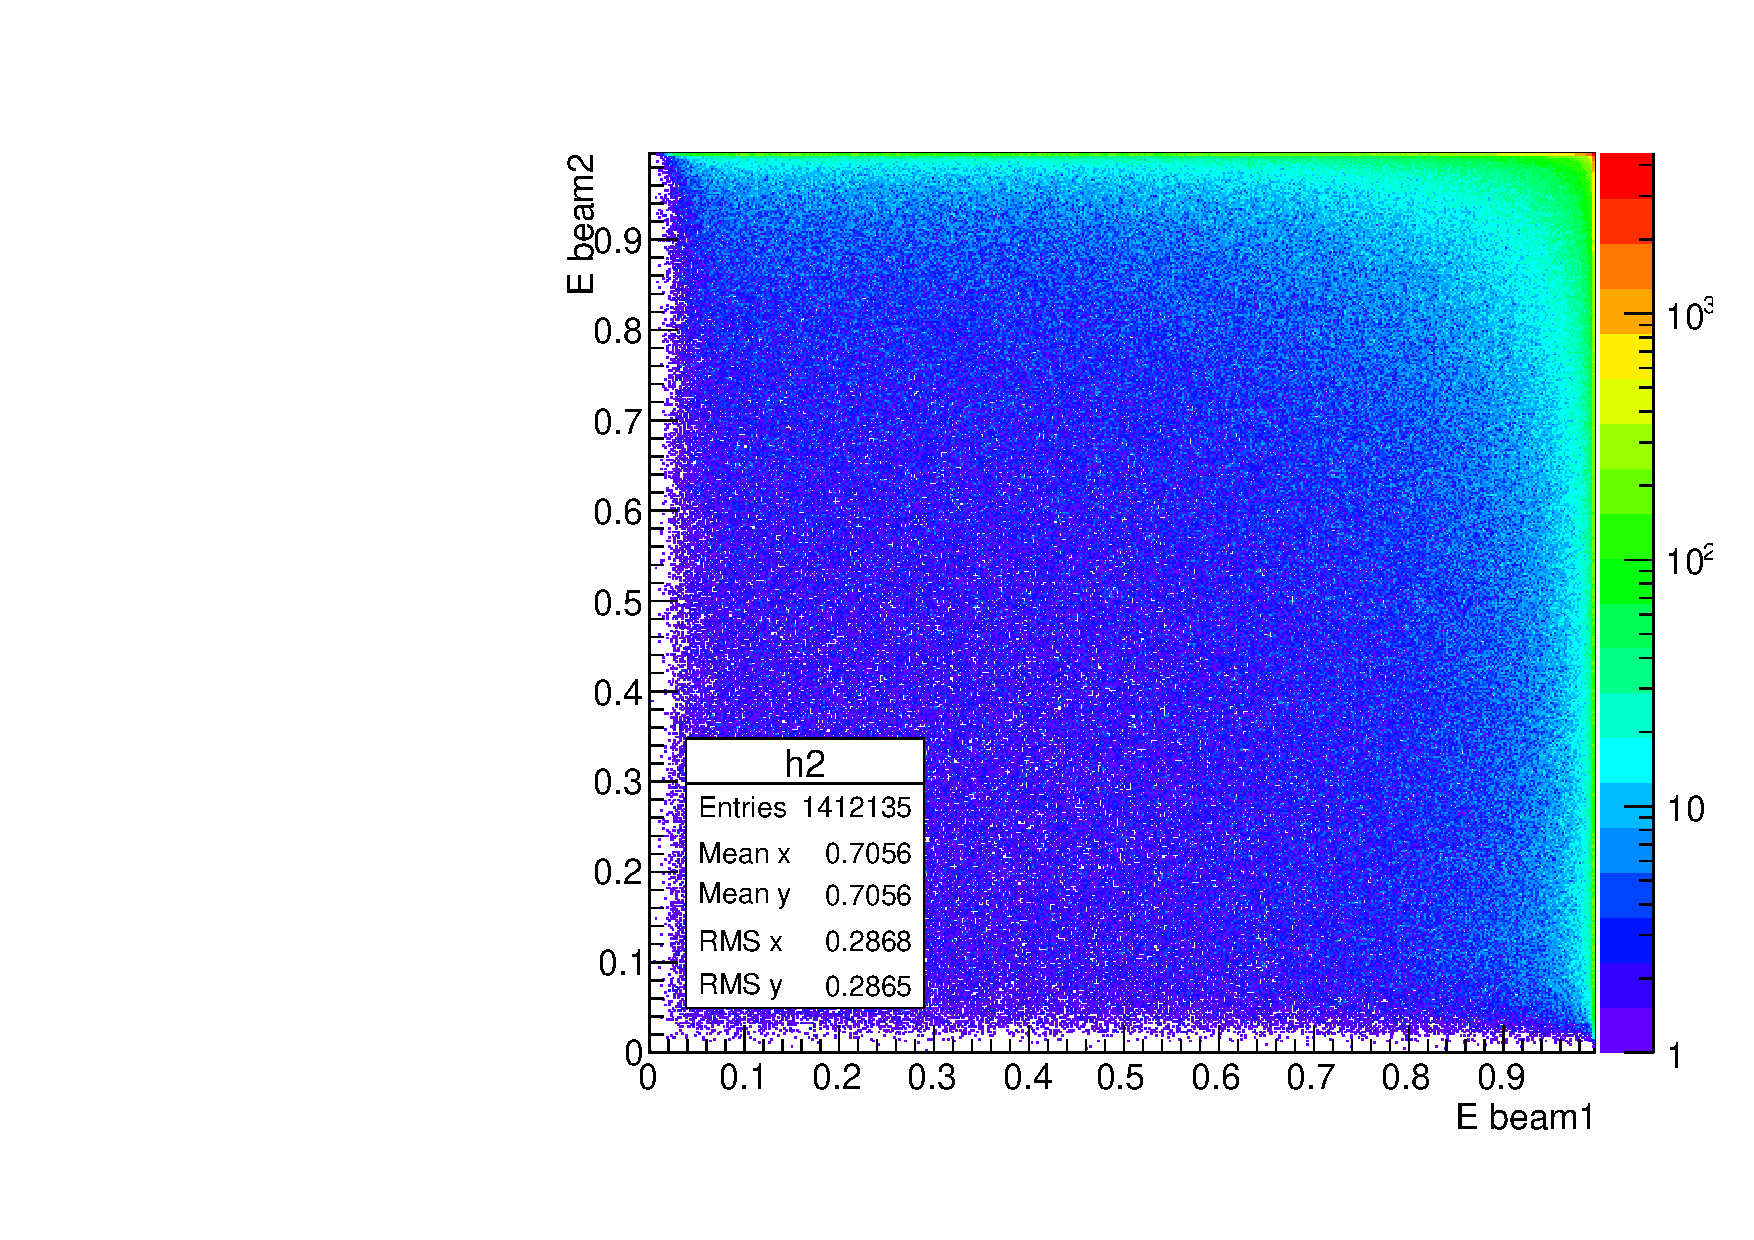
\includegraphics[width=6cm]{Body.pdf}
\end{center}
\end{frame}

\begin{frame}
\frametitle{Getting a model for the body}
\begin{columns}[c]
\column{6cm}
\begin{center}
Projection on E1:\\
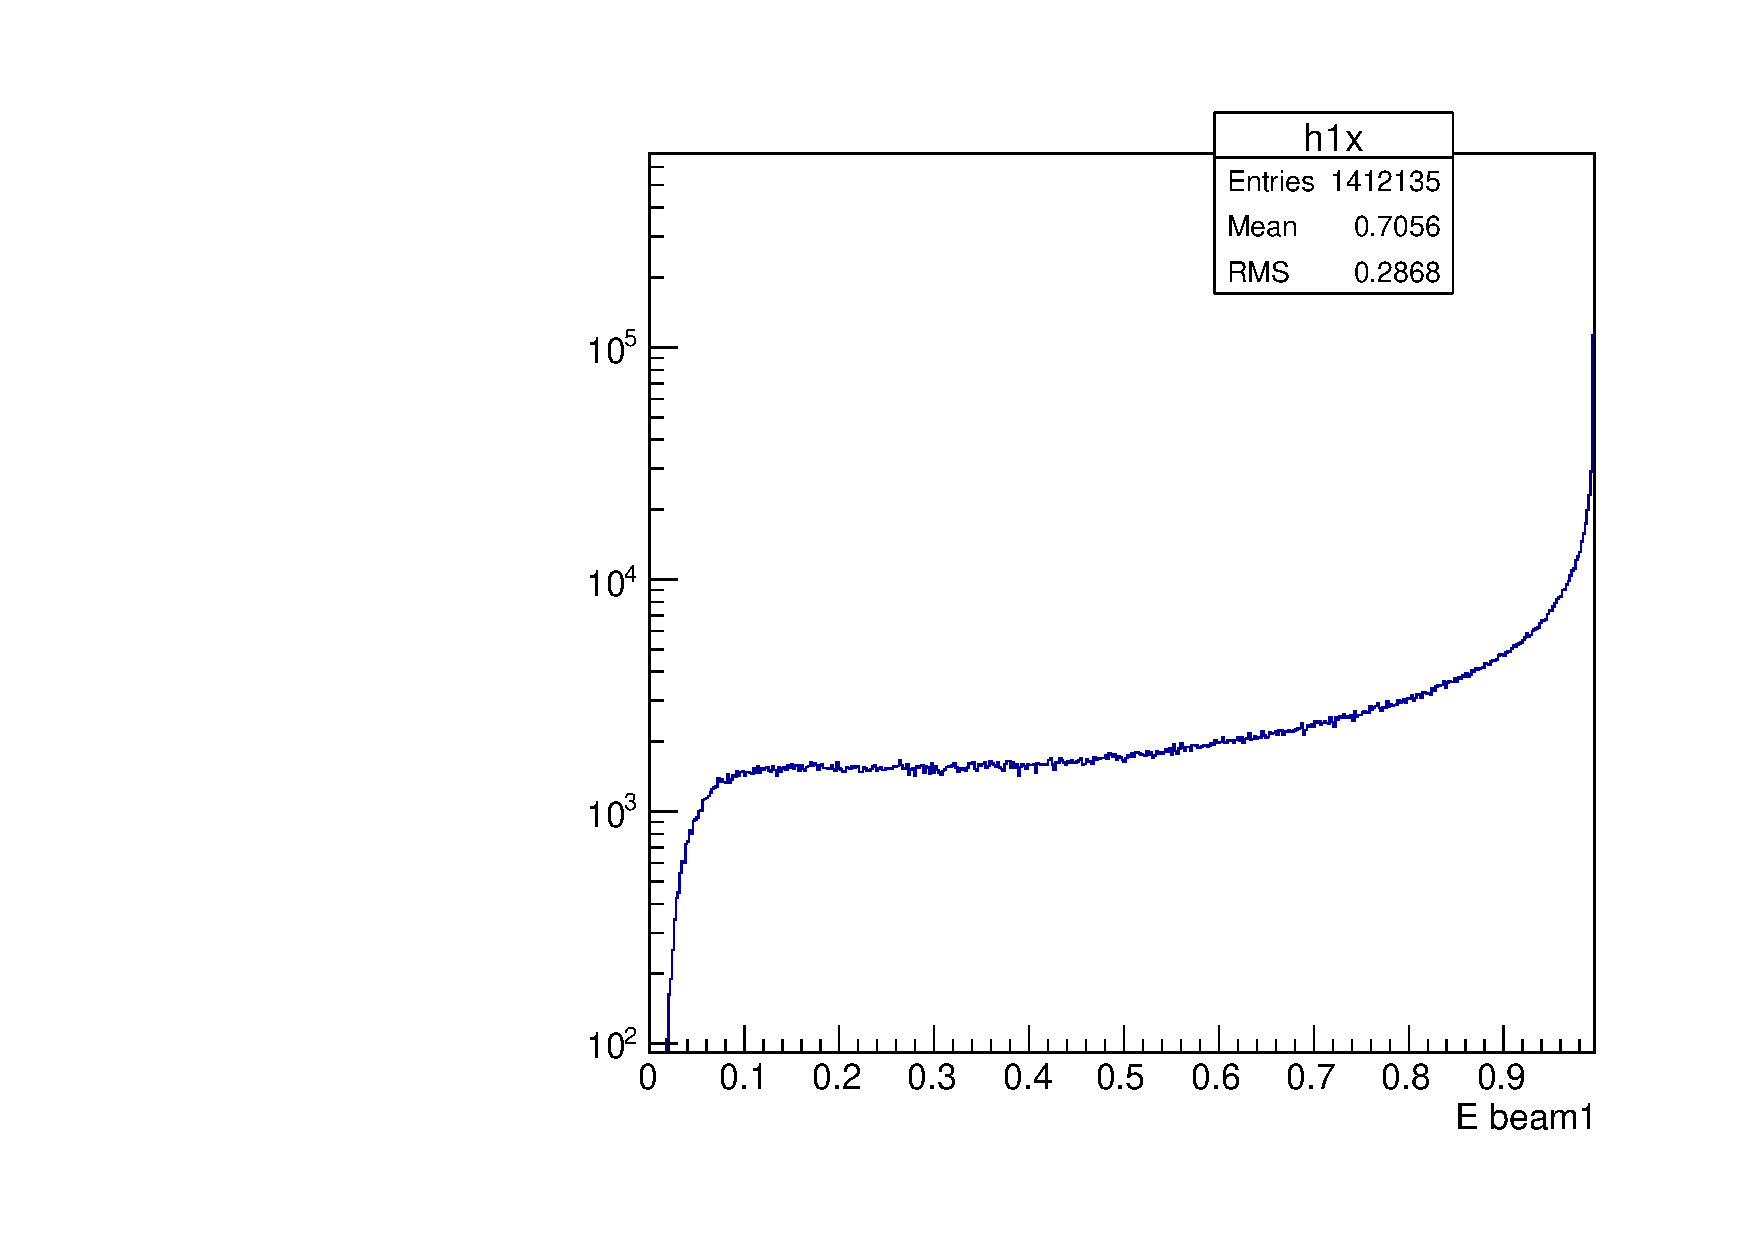
\includegraphics[width=4.5cm]{Body_projX.pdf}
\end{center}
\column{6cm}
\begin{center}
Projection on E2:\\
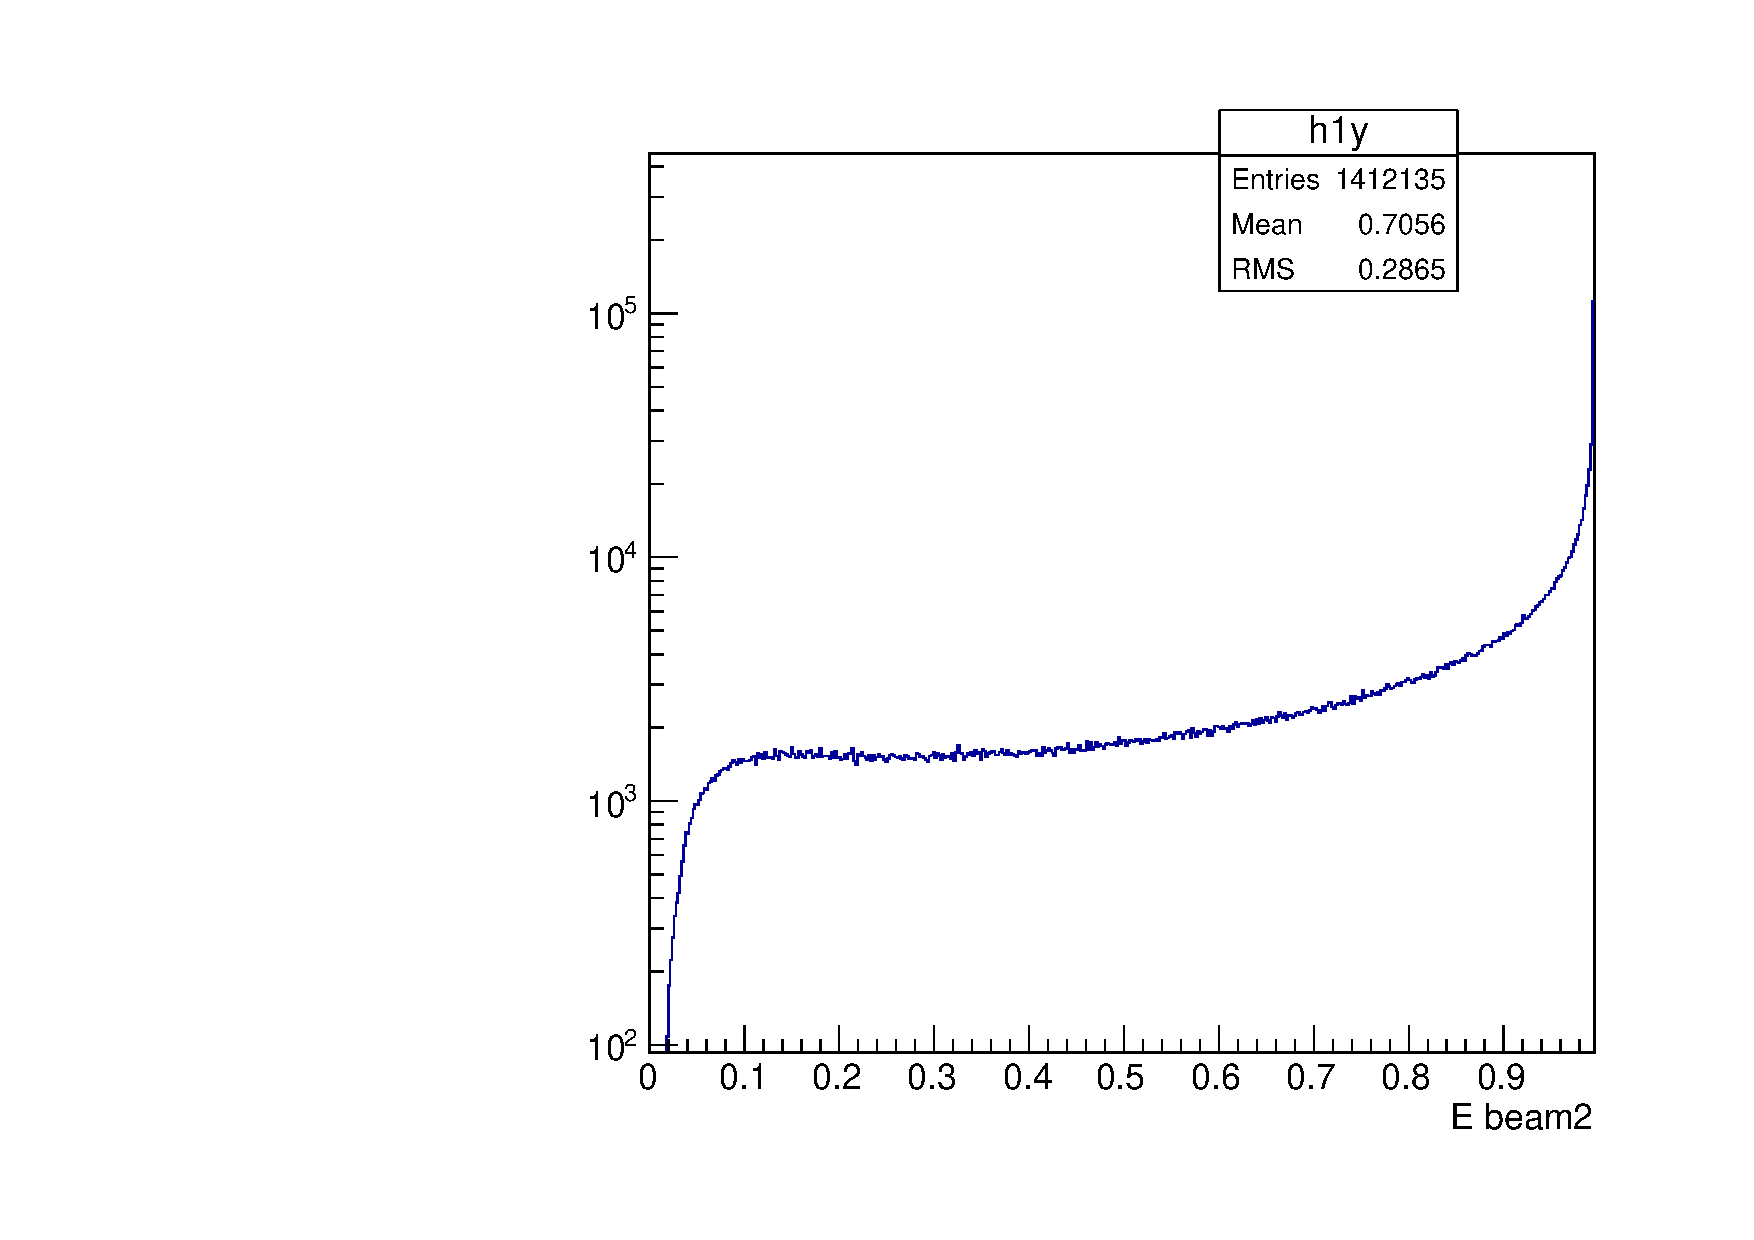
\includegraphics[width=4.5cm]{Body_projY.pdf}
\end{center}
\end{columns}
Body is assumed to be dominated by beamstrahlung effects. The beam spread is
completely neglected.\\
~\\
Beamstrahlung is modeled by different beta distributions
for each beam (slide~\ref{slide:betadiststra}).
\end{frame}

\begin{frame}
\frametitle{Final model}
Global factor for every regions: 3 parameters\\
2 Beam spread beta function for the peak: 4 parameters\\
%2 Beam spread beta functions for the body: 4 parameters\\
2 Beamstrahlung beta functions for the body: 4 parameters\\
1 Beam spread for each arm: 4 parameters\\
\alert{15 free parameters}.
\end{frame}

\section{Statistical Intermission}
\begin{frame}
\frametitle{Statistical Methodology: the $\chi^2$}
Method relies on histogram comparison using $\chi^2$. To be a correct estimator
of the compatibility\footnote{Statistical Methods for 
Experimental Physics, F. James, p.304}:
\begin{itemize}
  \item Number of entries per bin $>7$
  \item Each bin should contain similar number of entries: equiprobability
  binning necessary (ROOT's TH2Poly only for 2D fit)
\end{itemize}
\begin{center}
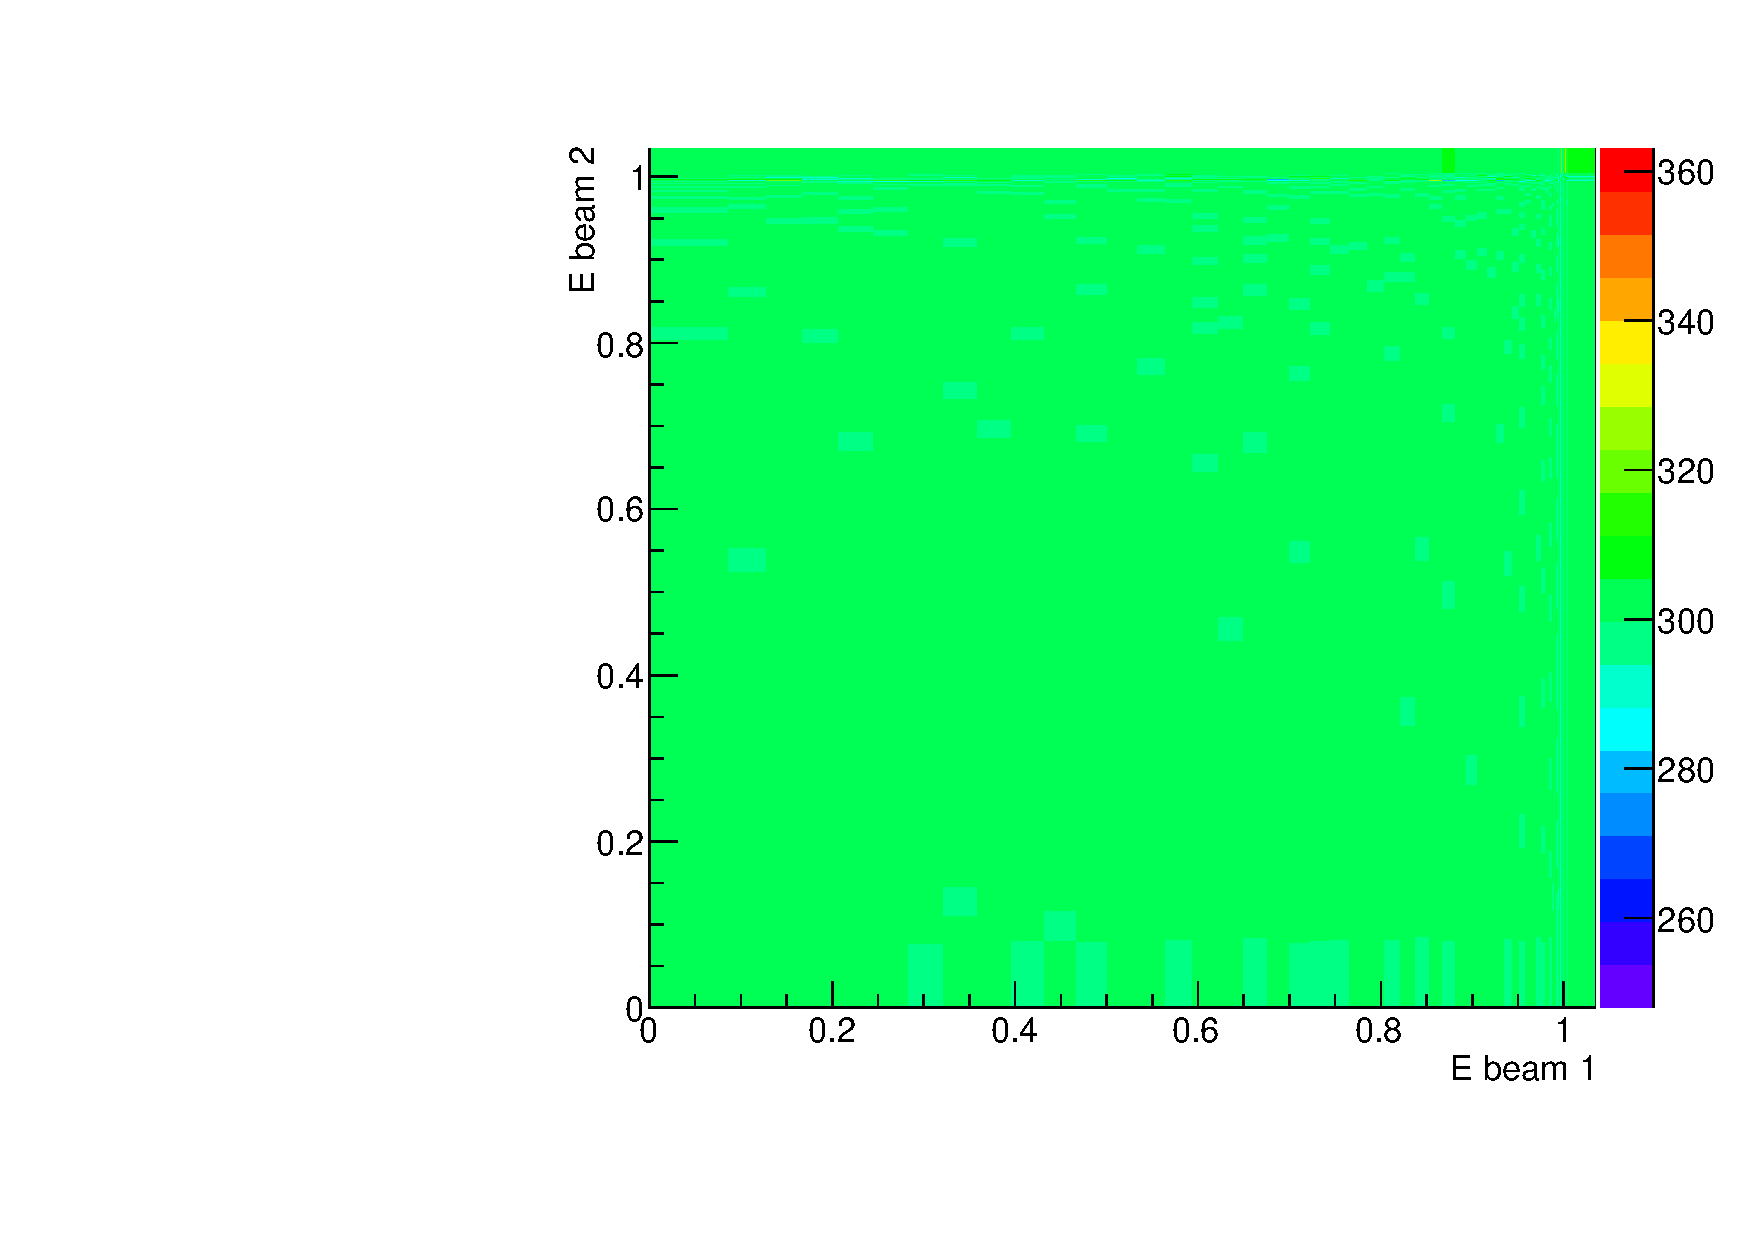
\includegraphics[width=5cm]{Th2PolyRef.pdf}
\end{center}
\end{frame}

\section{Fit Status}
\begin{frame}
\frametitle{Fit Status}
Model level fit: fit directly the beam energies\\
~\\
Ingredients:
\begin{itemize}
  \item Model: see before
  \item Data: 3\,000\,000 events of Guinea Pig (Data), 3\,000\,000 events of our
  model (Monte Carlo)
\end{itemize}
\end{frame}
\begin{frame}
\frametitle{Model level fit}
\begin{center}
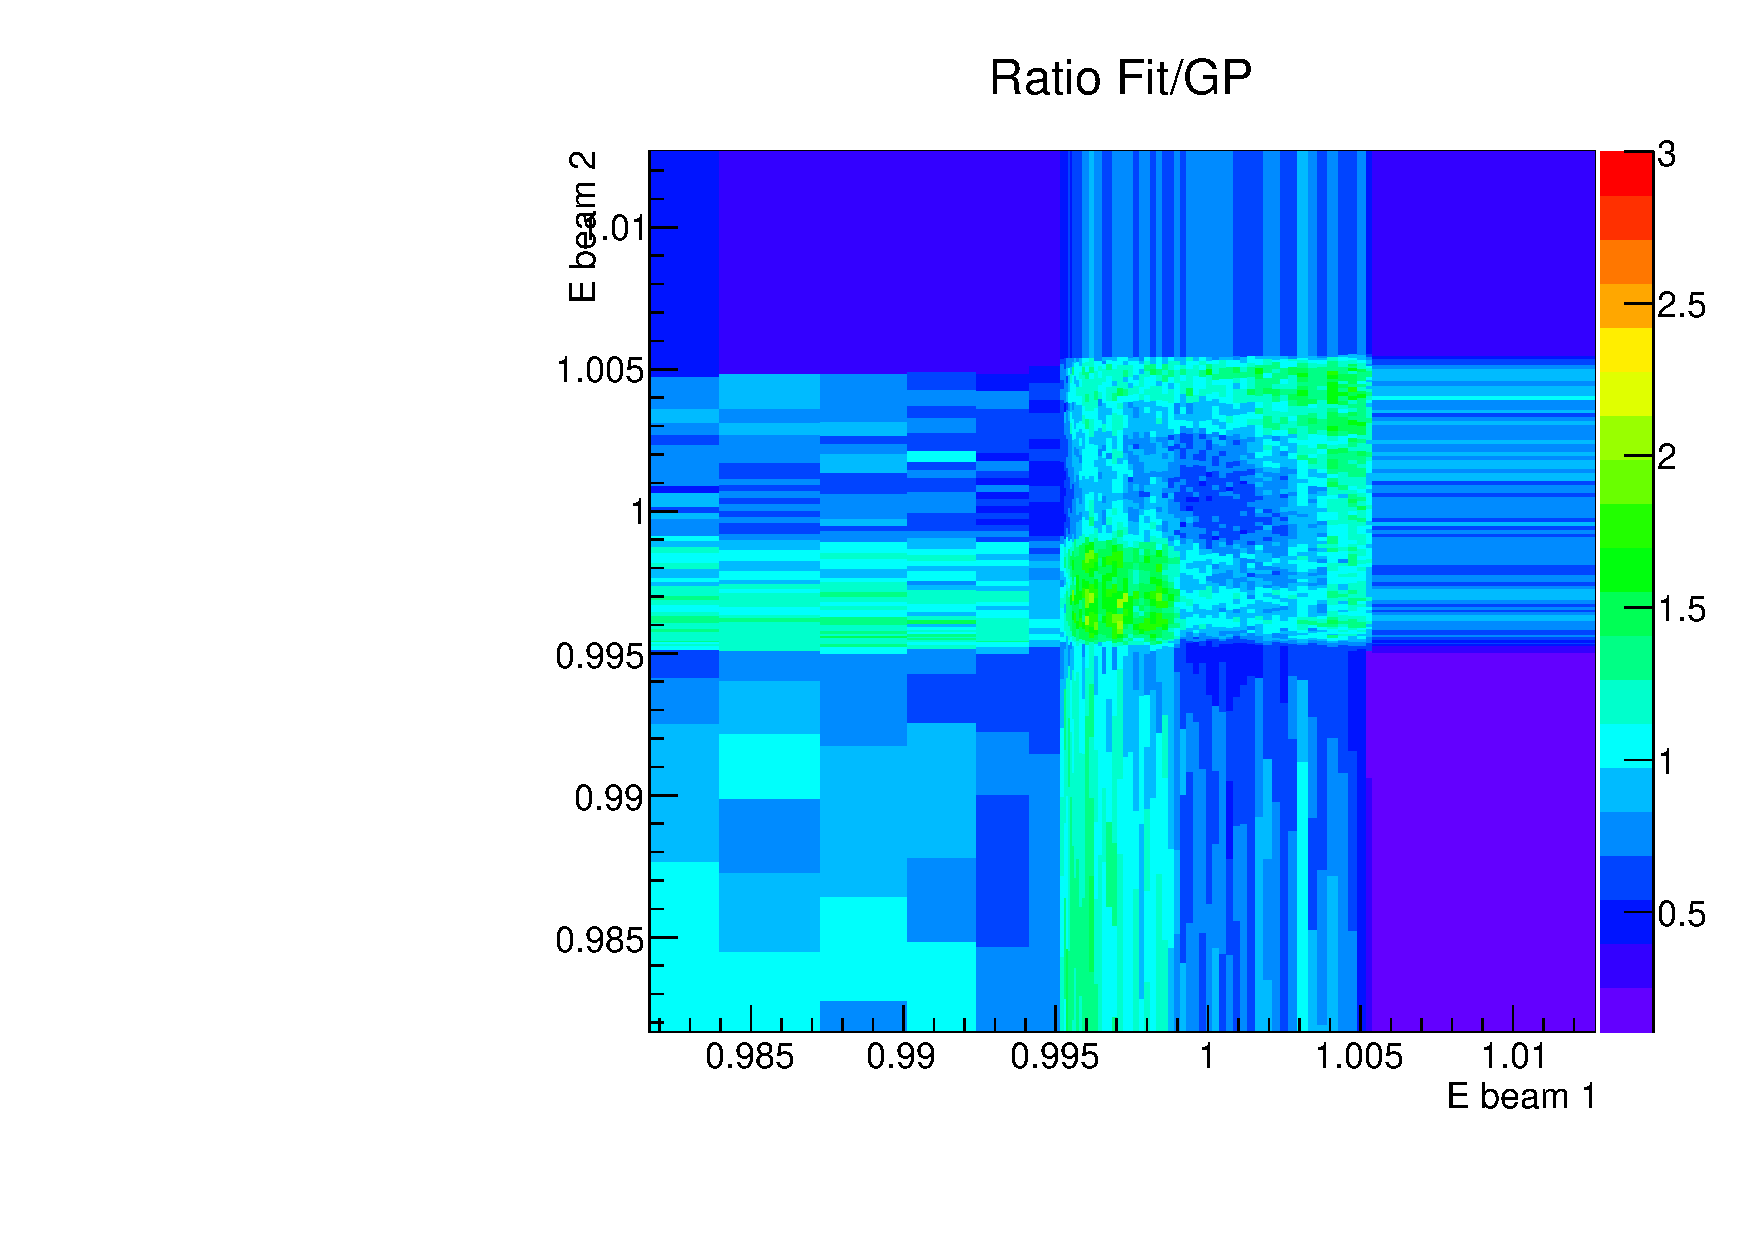
\includegraphics[width=9cm]{Ratio_Fit_vs_GP_FCAL.pdf}
\end{center}
\end{frame}
\begin{frame}
\frametitle{Fit result}
\begin{columns}[c]
\column{6cm}
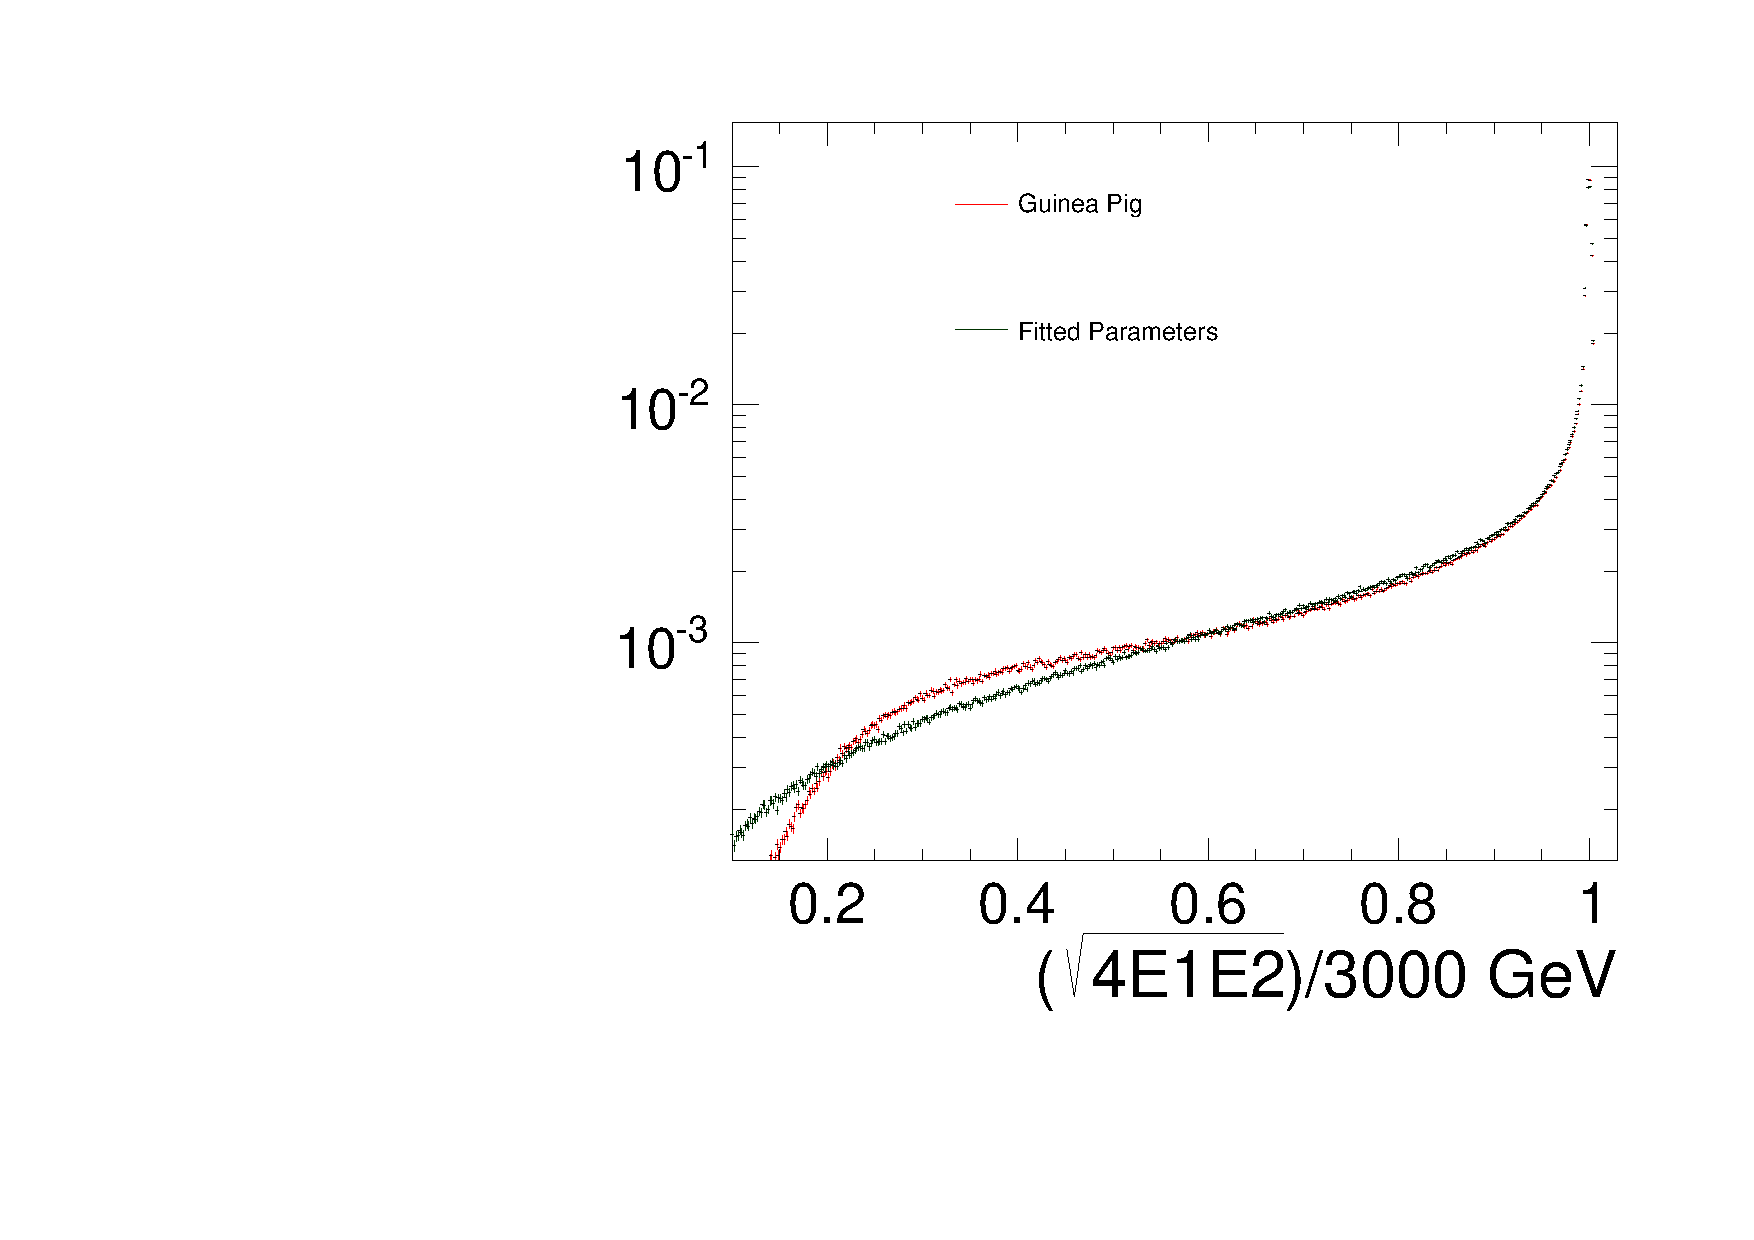
\includegraphics[width=6cm]{FullSpectrumFCAL.pdf}
\column{6cm}	
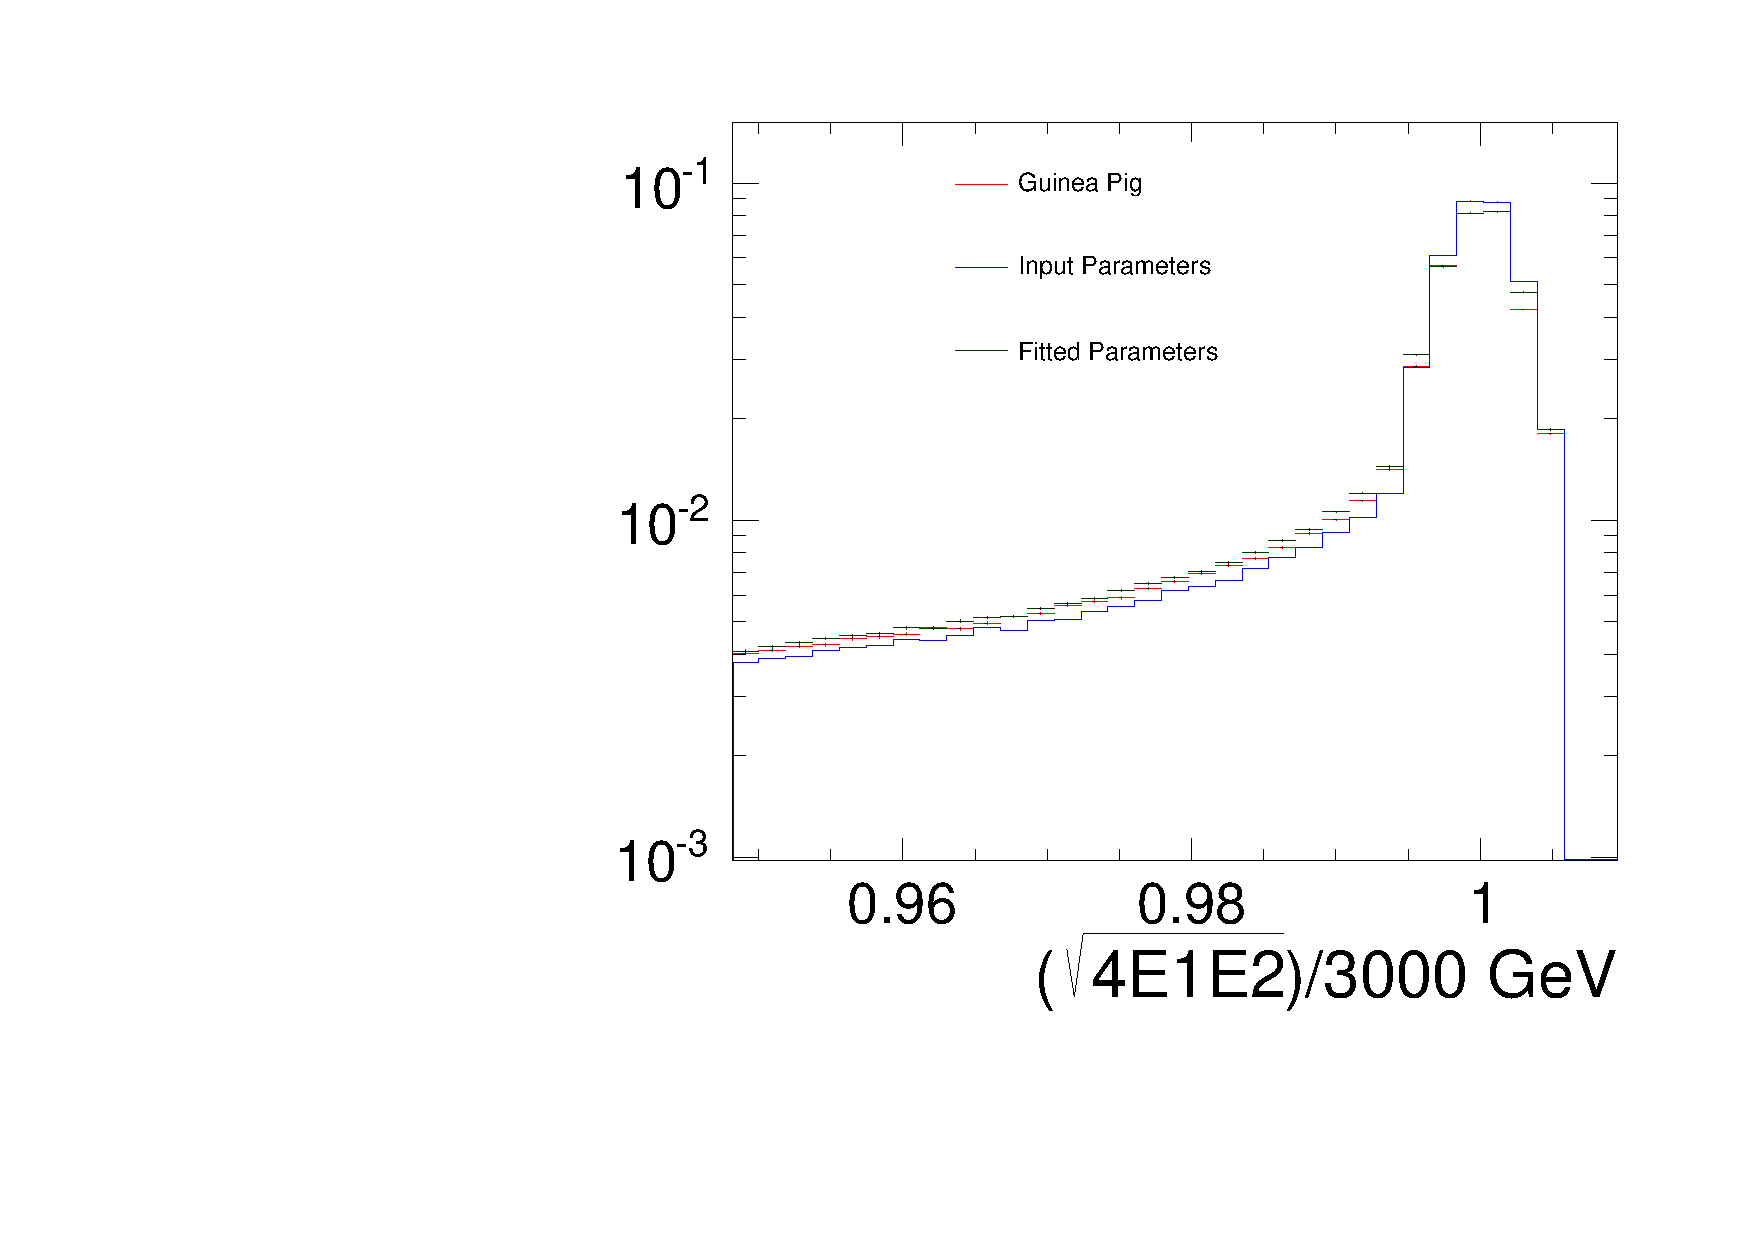
\includegraphics[width=6cm]{FullSpectrumFCAL_zoom.pdf}
\end{columns}
See backup for linear scale plots.
\end{frame}
\begin{frame}
\frametitle{Fit result}\label{slide:fitres}
Relative difference between the fitted parameter set and Guinea Pig:
\begin{columns}[c]
\column{6cm}
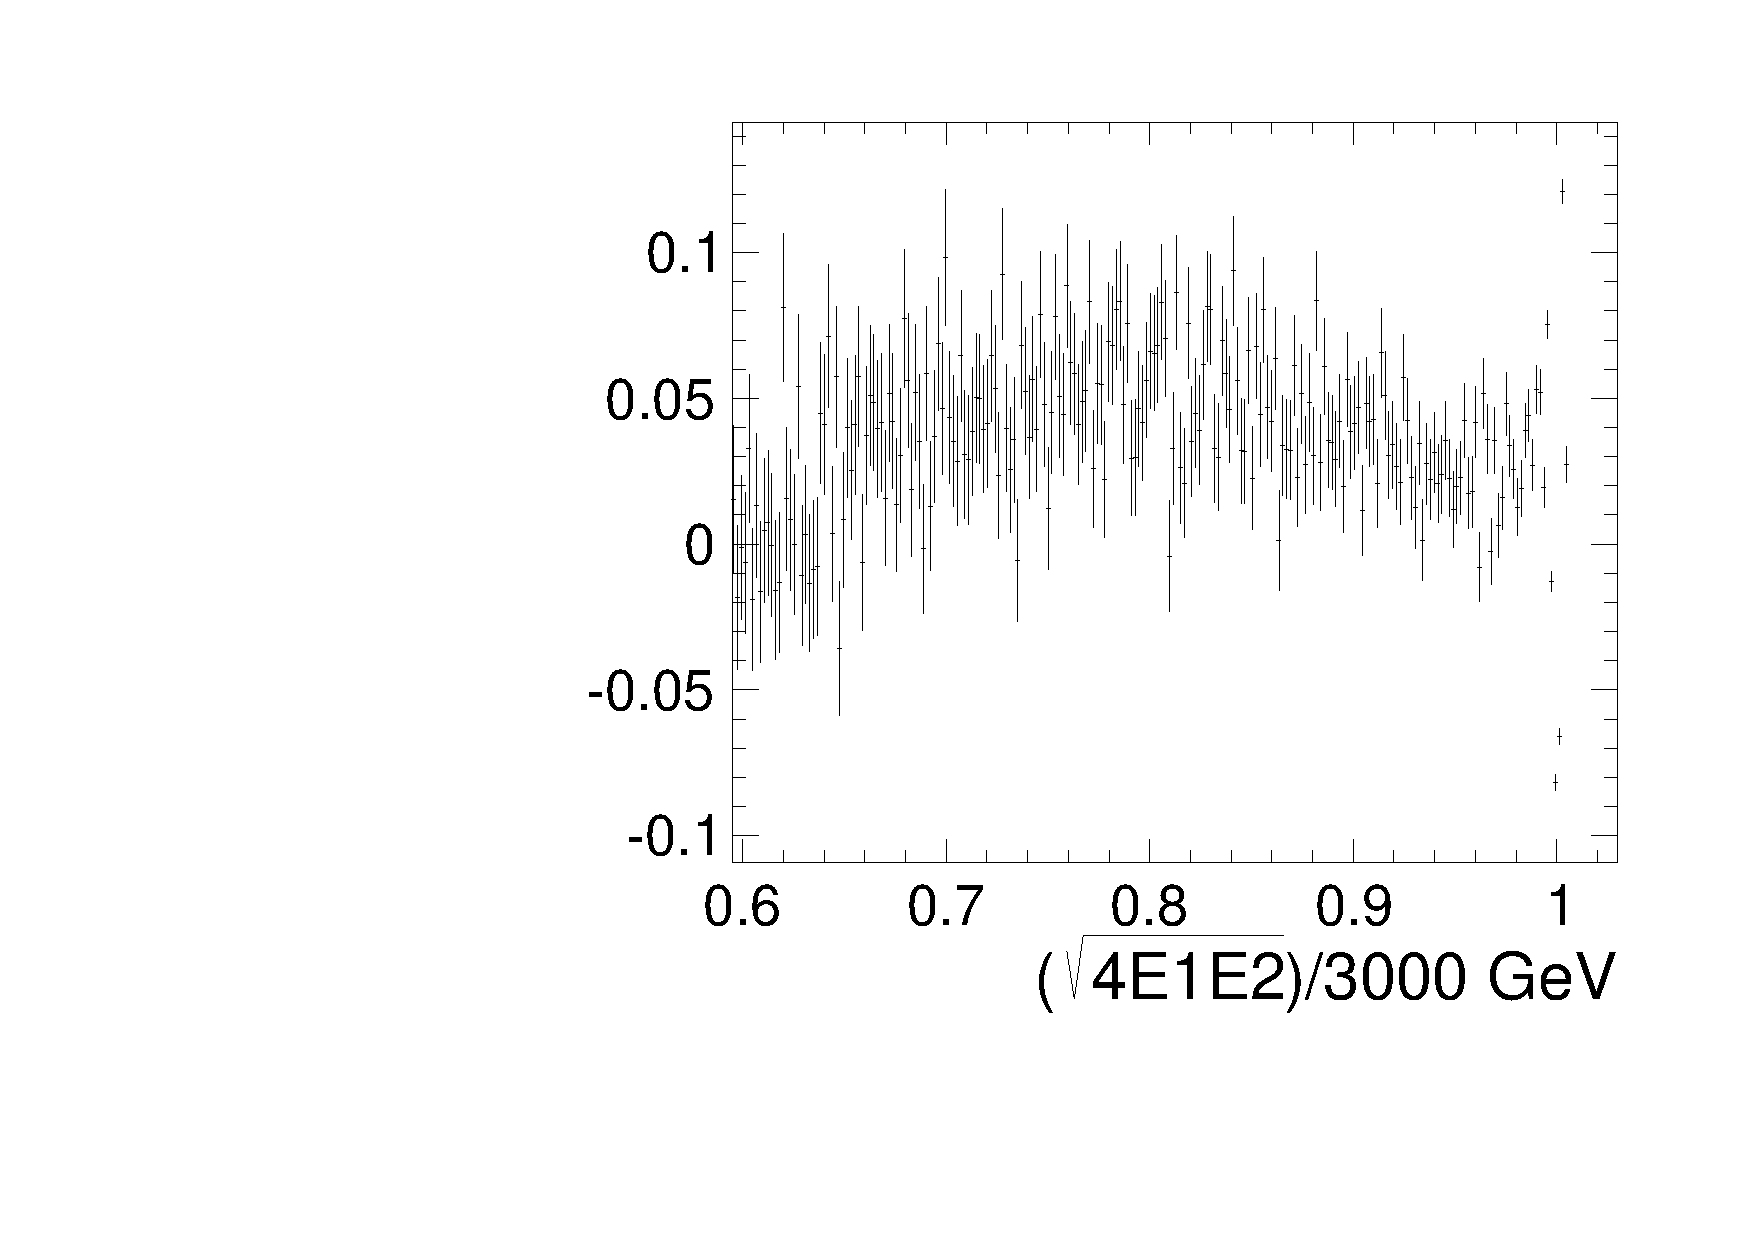
\includegraphics[width=6cm]{Relative_diff_Fit_GP.pdf}
\column{6cm}
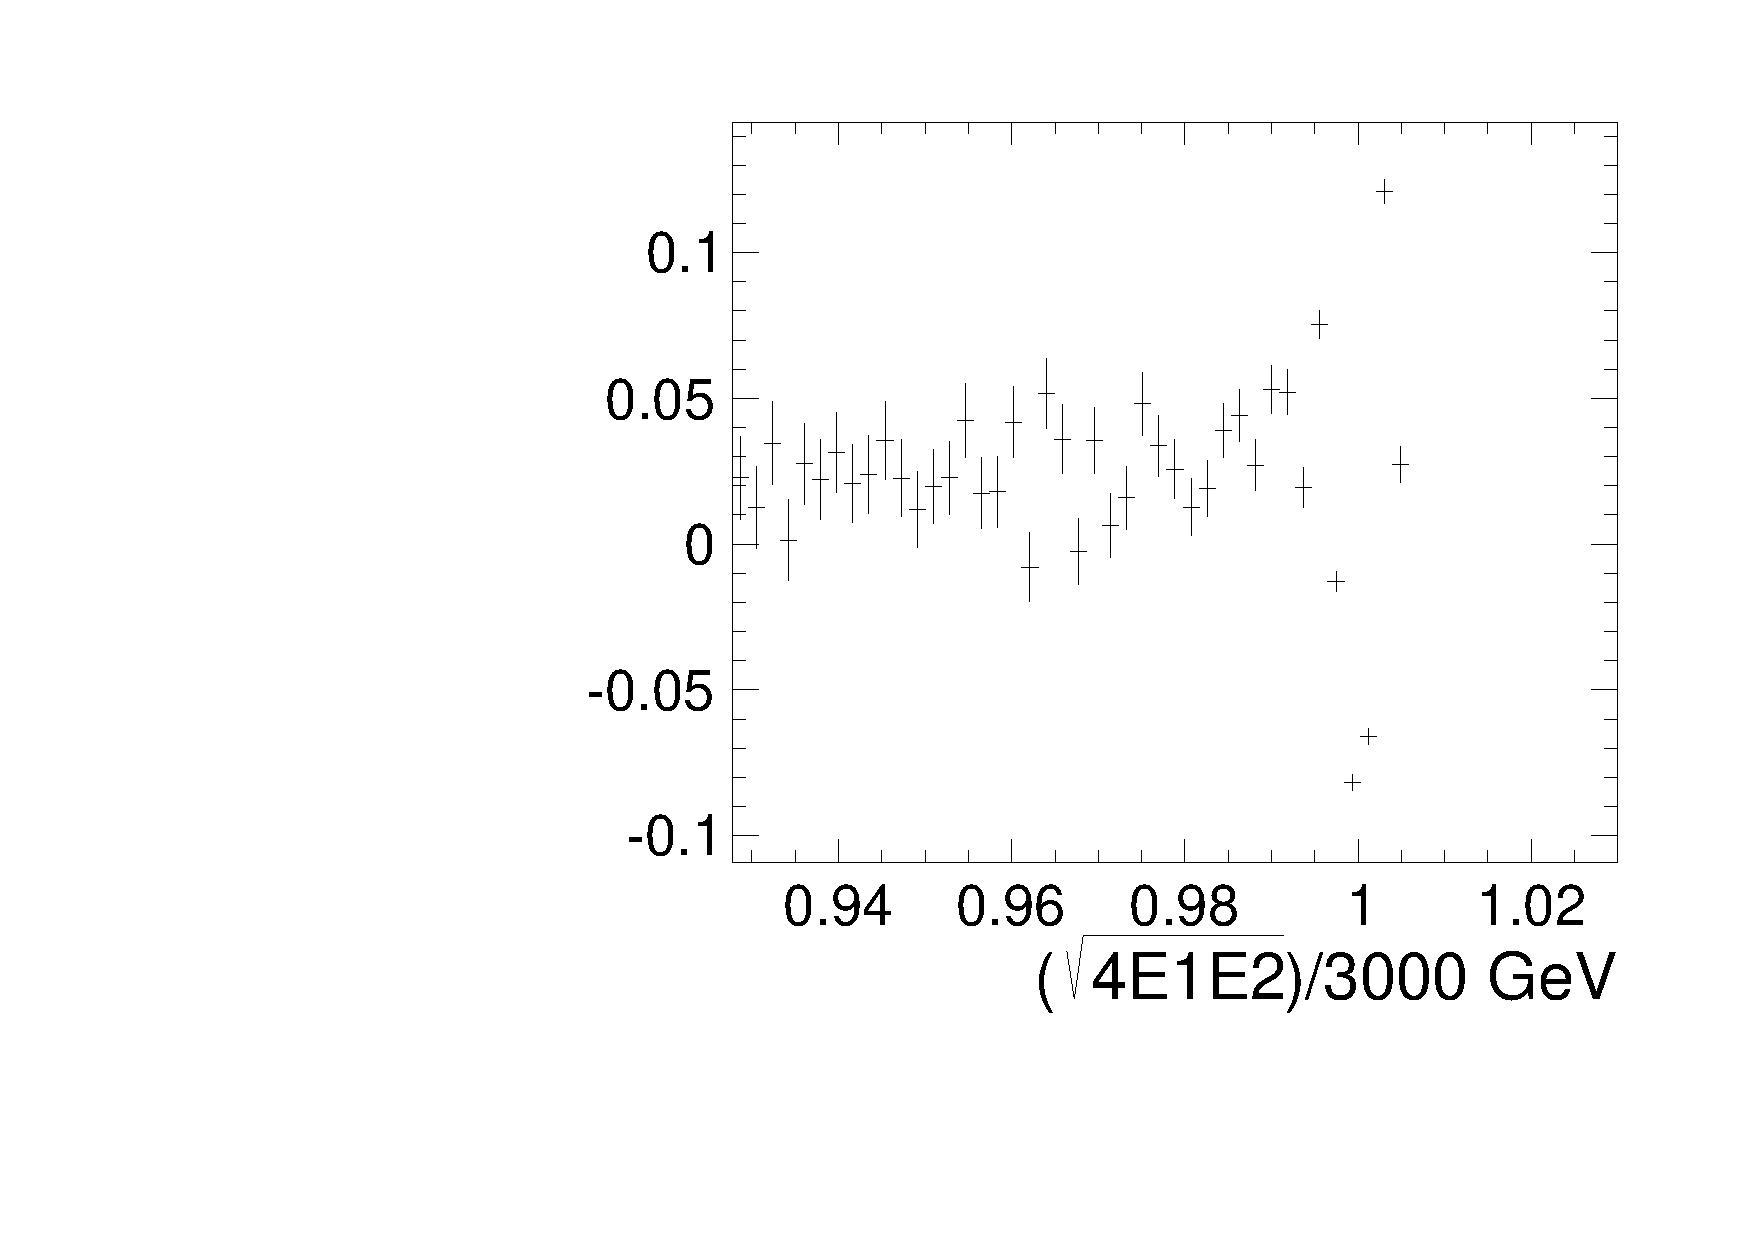
\includegraphics[width=6cm]{Relative_diff_Fit_GP_zoom.pdf}
\end{columns}
\end{frame}

\begin{frame}
\frametitle{Partial conclusion}
Fit at model level not perfect:
\begin{itemize}
  \item Need to improve model: beta distributions for the peak and the arms not
  fully suitable, need \alert{higher order objects} (more parameters)
  \item For the beamstrahlung, more beta functions may be needed
\end{itemize} 
~\\
Meanwhile: can in parallel setup framework for \alert{Bhabha events}.
\end{frame}

\section{Fit with Bhabha Events}
\begin{frame}
\frametitle{Bhabha events}
Using \alert{BHWide} to obtain large angle Bhabha events:
\begin{itemize}
  \item Input energies given either by Guinea Pig or by our model: gives 2
  samples
  \item Keep only the particles with $\theta>7^\circ$: visible in the
  tracking detector
\end{itemize}
~\\
Until we have the full chain of simulation/reconstruction running, \alert{smear}
the \alert{measurable energies} (electron and positron) to ``simulate'' the
energy \alert{resolution} effects.
\end{frame}
\begin{frame}
\frametitle{Bhabha events}
\begin{columns}[c]
\column{6cm}
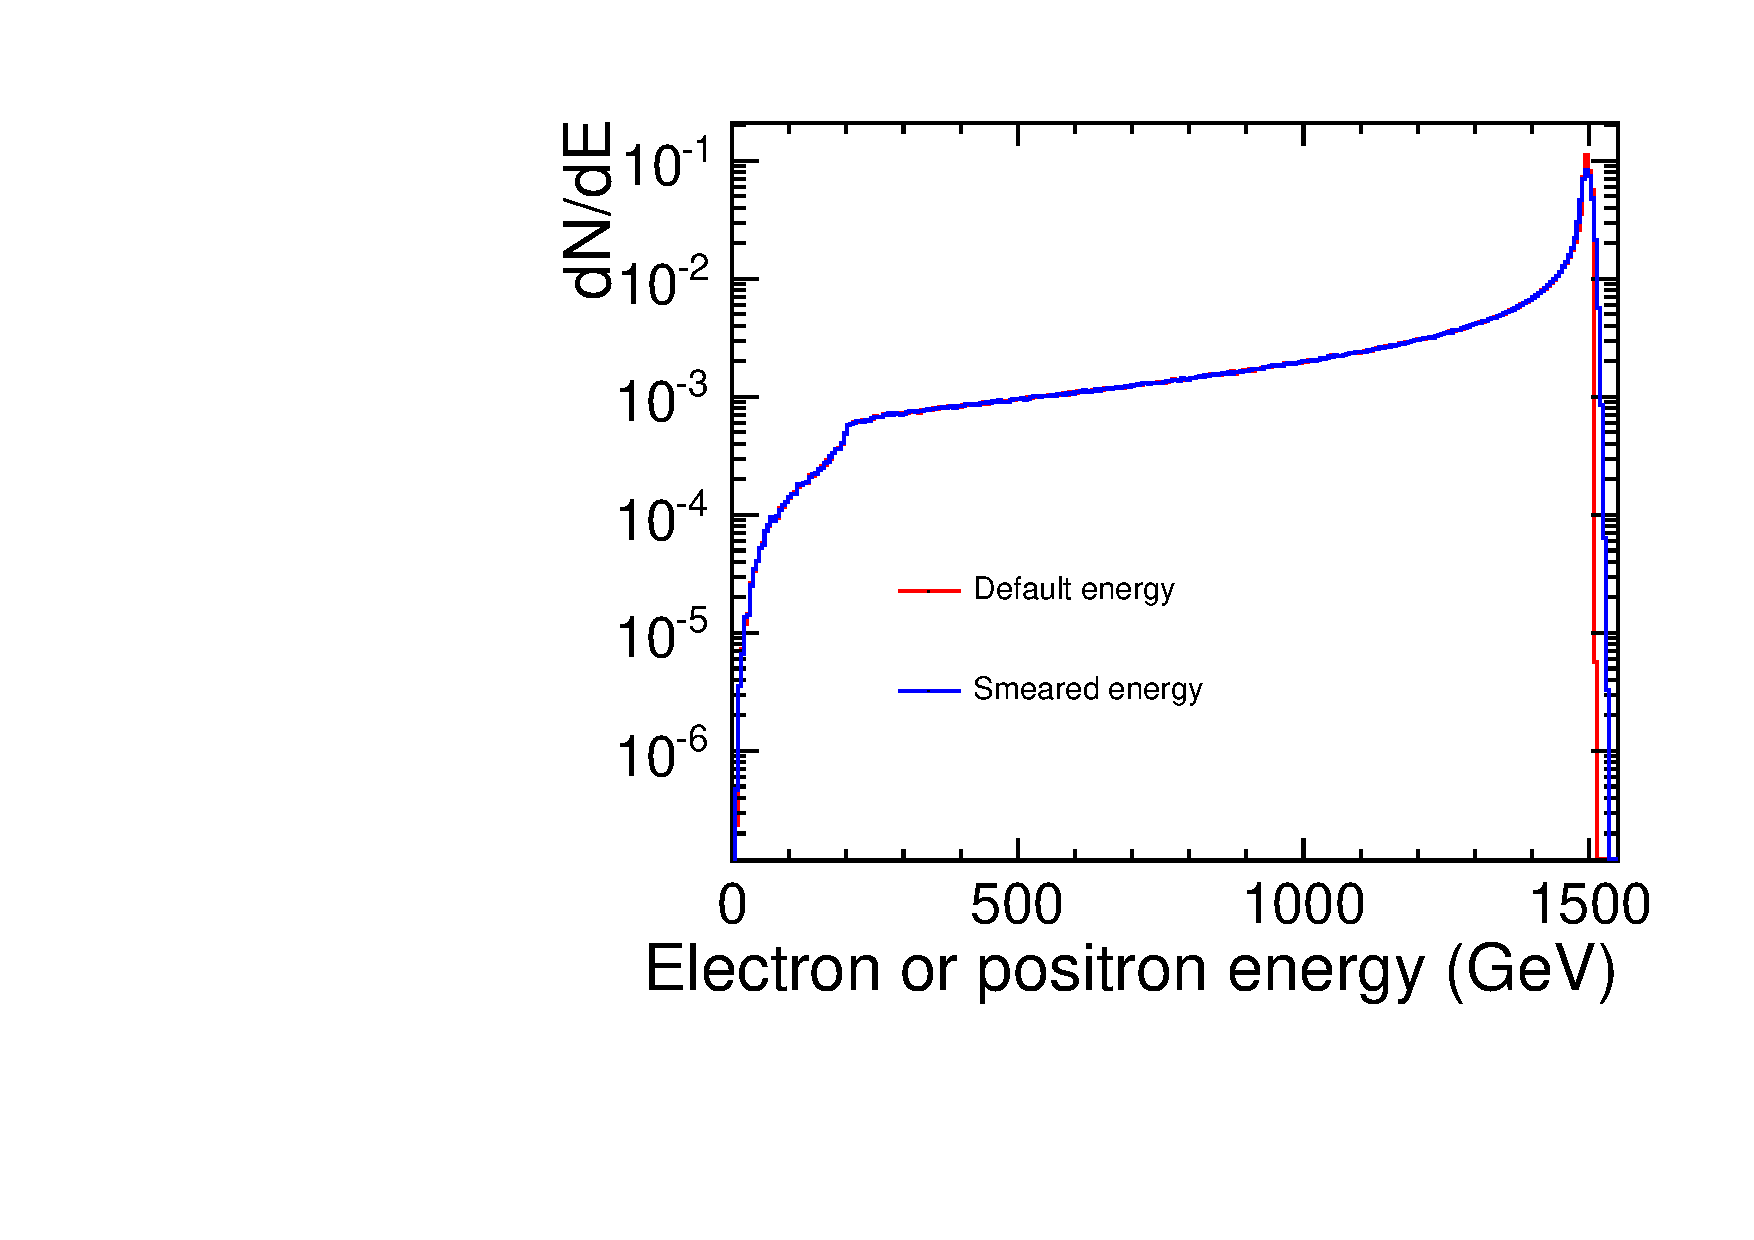
\includegraphics[width=6cm]{ElectronEnergyFCAL.pdf}
\column{6cm}
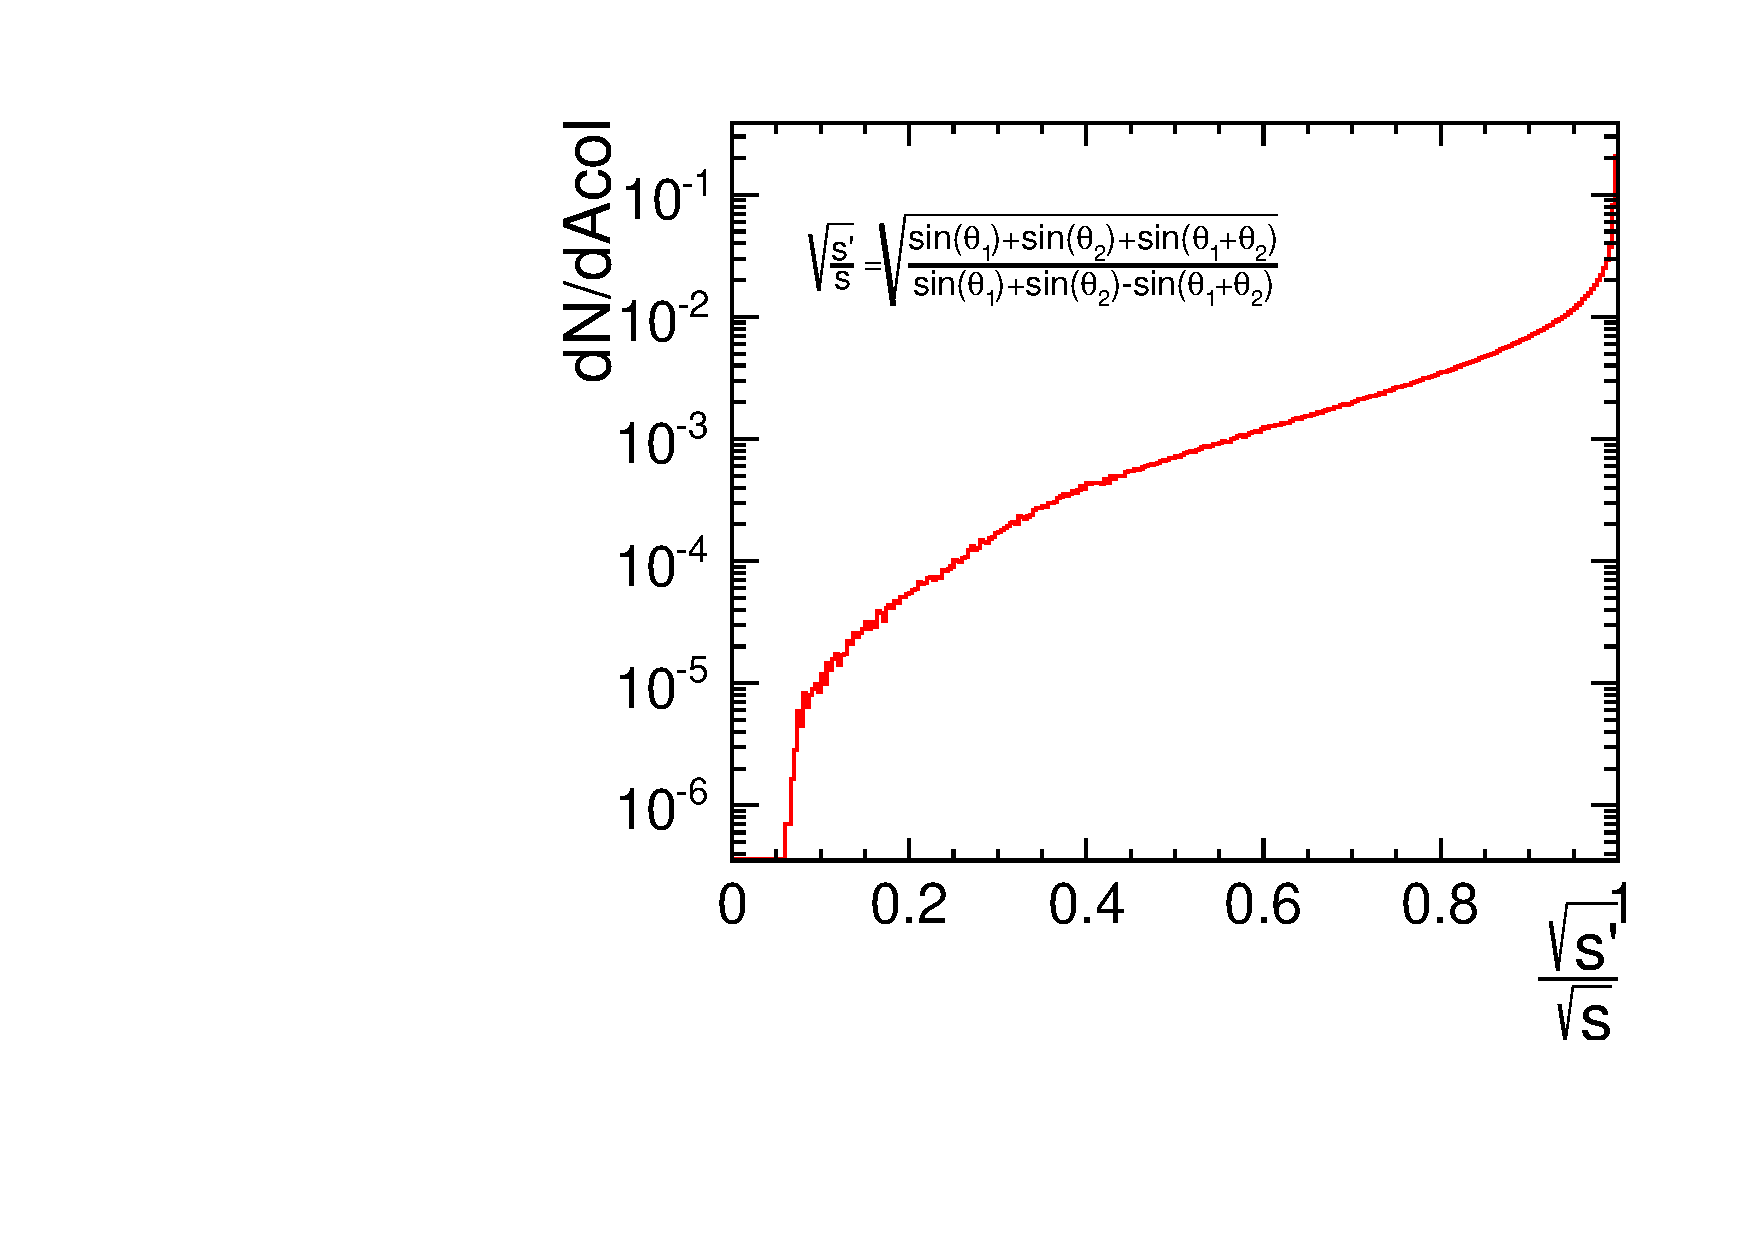
\includegraphics[width=6cm]{AccolinearityFCAL.pdf}
\end{columns}
\end{frame}

\begin{frame}
\frametitle{Fitting the Bhabha events}
Reweighting fit works as long as the input beam energies are kept in the
generator level (BHWide) file:
\begin{itemize}
  \item 1 event is then parametrized by
  $\{E_{beam1},E_{beam2},E_{p},E_{e},\frac{\sqrt{s'}}{\sqrt{s}}\}$
  \item Use $\{E_{beam1},E_{beam2}\}$ for the weight computation
  \item Use $\{E_{p},E_{e},\frac{\sqrt{s'}}{\sqrt{s}}\}$ for Data comparison: 3D
  histogram needed
  \item Resolution effect canceled out as long as they are identical between
  Data and MC (systematics), but more events needed to compensate.
\end{itemize}
~\\
Issue: defining equiprobability binning in 3D\\
~\\
Now do not use equiprobability binning, throw away bins with less than 10
entries.\\
~\\
Nothing to show yet: \alert{work in progress}.
\end{frame}

%\begin{frame}
%\frametitle{Preliminary fit status on Bhabha events}

%\end{frame}

\section{Conclusion}
\begin{frame}
\frametitle{Conclusion}
Status:
\begin{itemize}
  \item Model level fitting in place, how can we improve?
  \item Framework setup
  \item Bhabha procedure exists, need improvement in binning
\end{itemize}
~\\
Things to add:
\begin{itemize}
  \item Full simulation and reconstruction
  \item Background handling: pairs, $\gamma\gamma \to had$, etc.
  \item Propagation of the errors on our parameters to the physics measurements
  and impacts
\end{itemize}
\end{frame}

\appendix
\begin{frame}
\frametitle{Backup slides}
\end{frame}
\begin{frame}
\frametitle{Brute force fit}
\begin{figure}[h]
  \begin{tikzpicture}[scale=2.8,auto]
\uncover<1-2>{\node [autoblock] (start) {\scriptsize Start: $[p]_0$};}
\uncover<2->{\node [block, below of=start, color=blue] (gen) {\scriptsize Generate Event with $[p]_N$: E1,E2};}
\uncover<3-10,12->{\node [autoblock, right of=gen] (bhwide) {\scriptsize
BHWide};} 
\uncover<4-10,13->{\node [autoblock, right of=bhwide] (sim) {\scriptsize
Simulation};} 
\uncover<5-10,14->{\node [autoblock, right of=sim] (rec) {\scriptsize
Reconstruction};} 
\uncover<6-10,15->{\node [block, below of=rec, color=red] (compare) {\scriptsize Compare with data: $\chi^2$};}
\uncover<7-10,16->{\node [decision, left of=compare, color=violet] (match)
{\scriptsize Minimum?};} 
\uncover<8-10,17->{\node [autoblock, below of=match] (done) {\scriptsize Done!};}
\uncover<9-11,18->{\node [block, below of=gen, color=magenta] (minim)
{\scriptsize Minimizer: $[p]_N \rightarrow [p]_{N+1}$};}	

\uncover<1-2>{\path [line] (start) -- (gen);}
\uncover<3-10,12->{\path [line] (gen) -- (bhwide);}
\uncover<4-10,13->{\path [line] (bhwide) -- (sim);}
\uncover<5-10,14->{\path [line] (sim) -- (rec);}
\uncover<6-10,15->{\path [line] (rec) -- (compare);}
\uncover<7-10,16->{\path [line] (compare) -- (match);}
\uncover<8-10,17->{\path [line] (match) -- node [near start] {\scriptsize yes} (done);}
\uncover<9-10,18->{\path [line] (match) -- node [near start] {\scriptsize no} (minim);}
\uncover<10-11,19->{\path [line] (minim) -- (gen);}
%\uncover<20>{\path [dline] (gen) -| node [near start] {Model level fit}
%(compare);}
%\node (start) at (0,2) [draw] {Start};
%\node (gen) at (0,1) [draw] {Generate Event with $[P]_N$: E1,E2};
\end{tikzpicture}
\end{figure}

\uncover<19>{ This procedure would take $\sim200$ years (see
slide~\ref{slide:timing}).}
\end{frame}

\begin{frame}
\frametitle{Why does it take so long?}\label{slide:timing}
\begin{itemize}
  \item $5\,000\,000$ events, to generate, simulate, and reconstruct
  \item $4\,000$ function calls (loop) in the minimization
  \item 5 minutes per event in the simulation, 30 seconds for the reconstruction
  \item $1\,000$ jobs on the grid in parallel
\end{itemize}
\end{frame}

\begin{frame}
\frametitle{Accounting for the correlations}
\begin{itemize}
  \item Correlations $\Rightarrow$ convolution
  \item Too complex to do numerically, let alone analytically
\end{itemize}
How we do it:
\begin{itemize}
  \item Generate values from each of the functions, and the
  corresponding probability to obtain such values
  \item Add the values for each beam to obtain the total beam energy
  \item Multiply the probabilities to have the event probability
\end{itemize}
\end{frame}

\begin{frame}
\frametitle{Beta distributions: beamstrahlung}\label{slide:betadiststra}
Beta distribution : $x^a(1-x)^b$ 
\begin{center}
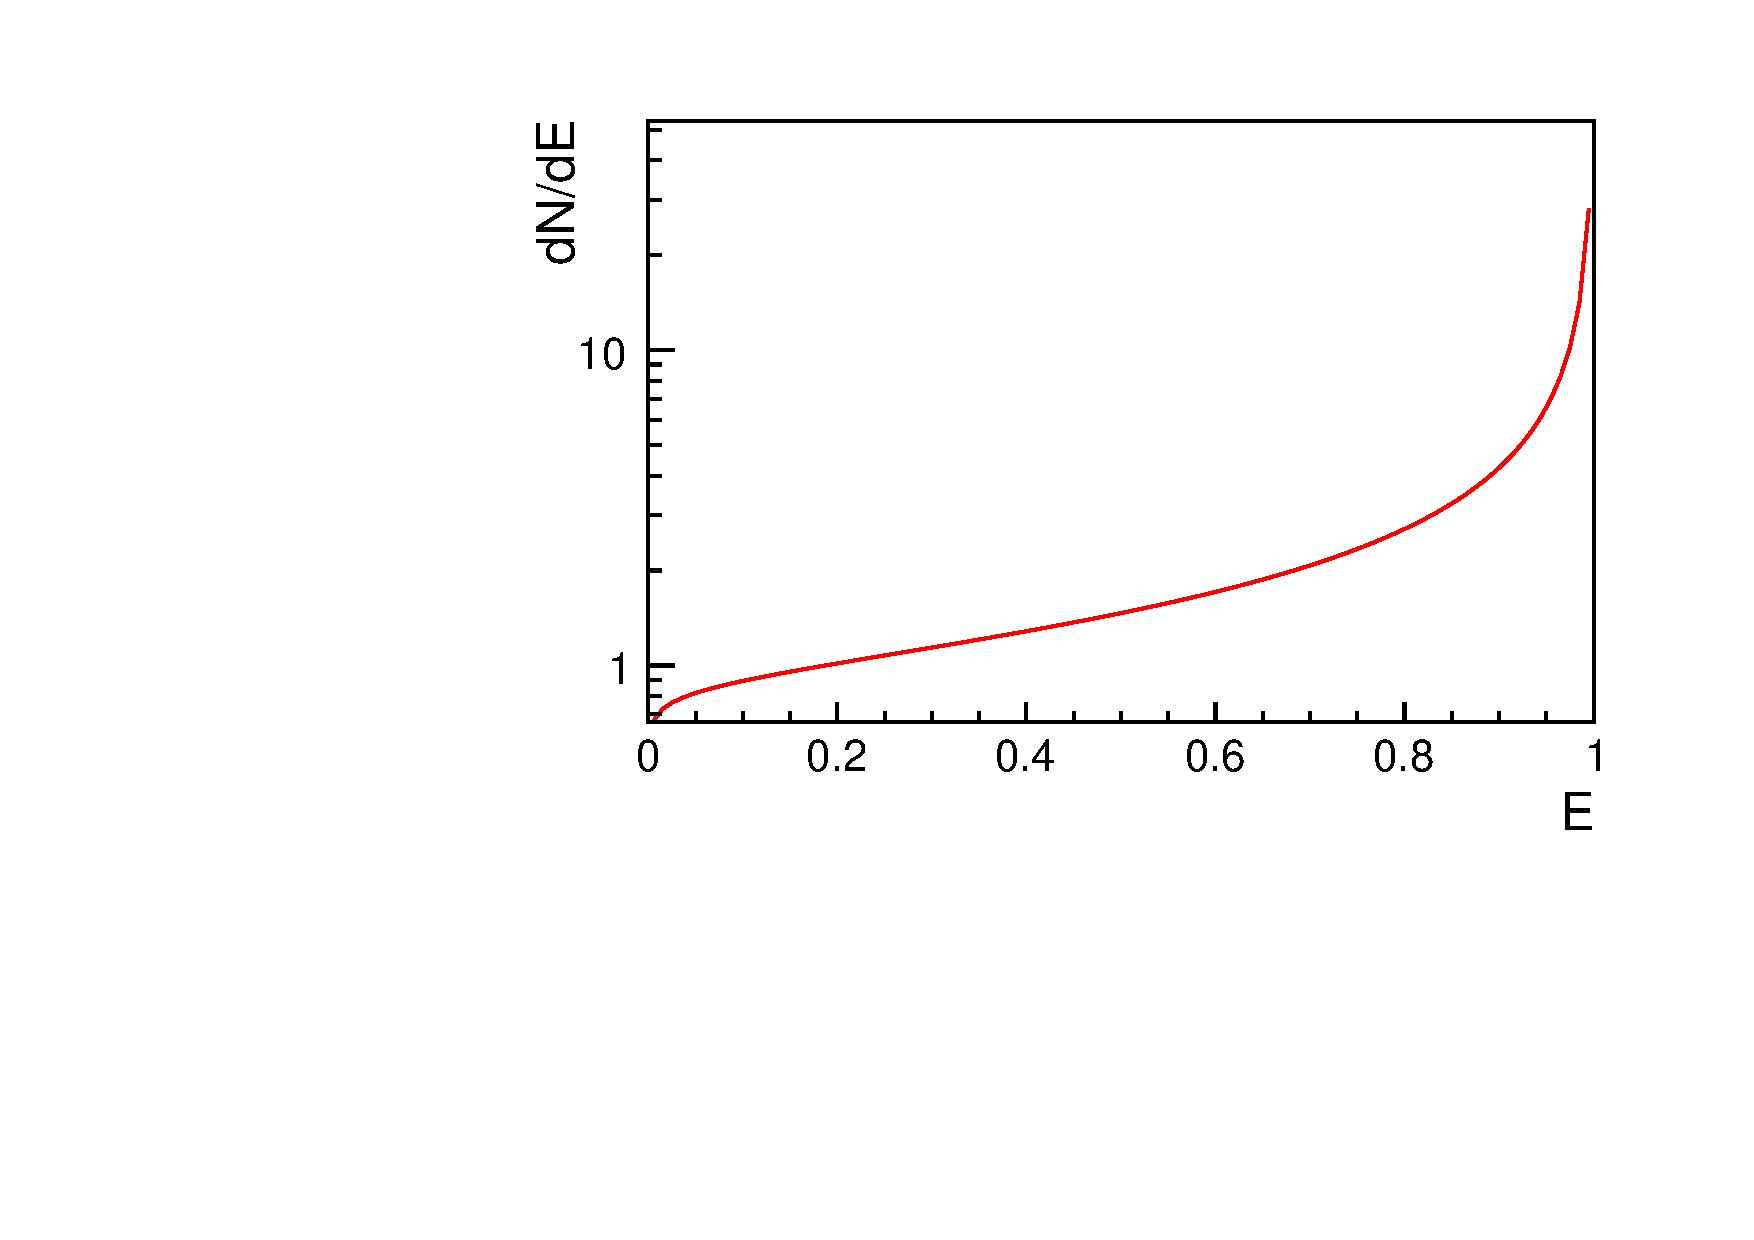
\includegraphics[width=9cm]{BetaFunction_beamstrahlung.pdf}\\
$a\sim0.08, b\sim-0.6$
\end{center}
\end{frame}

\begin{frame}
\frametitle{Beta distributions: beam spread in the
peak}\label{slide:betadistspreadpeak} 
Beta distribution : $x^a(1-x)^b$ 
\begin{center}
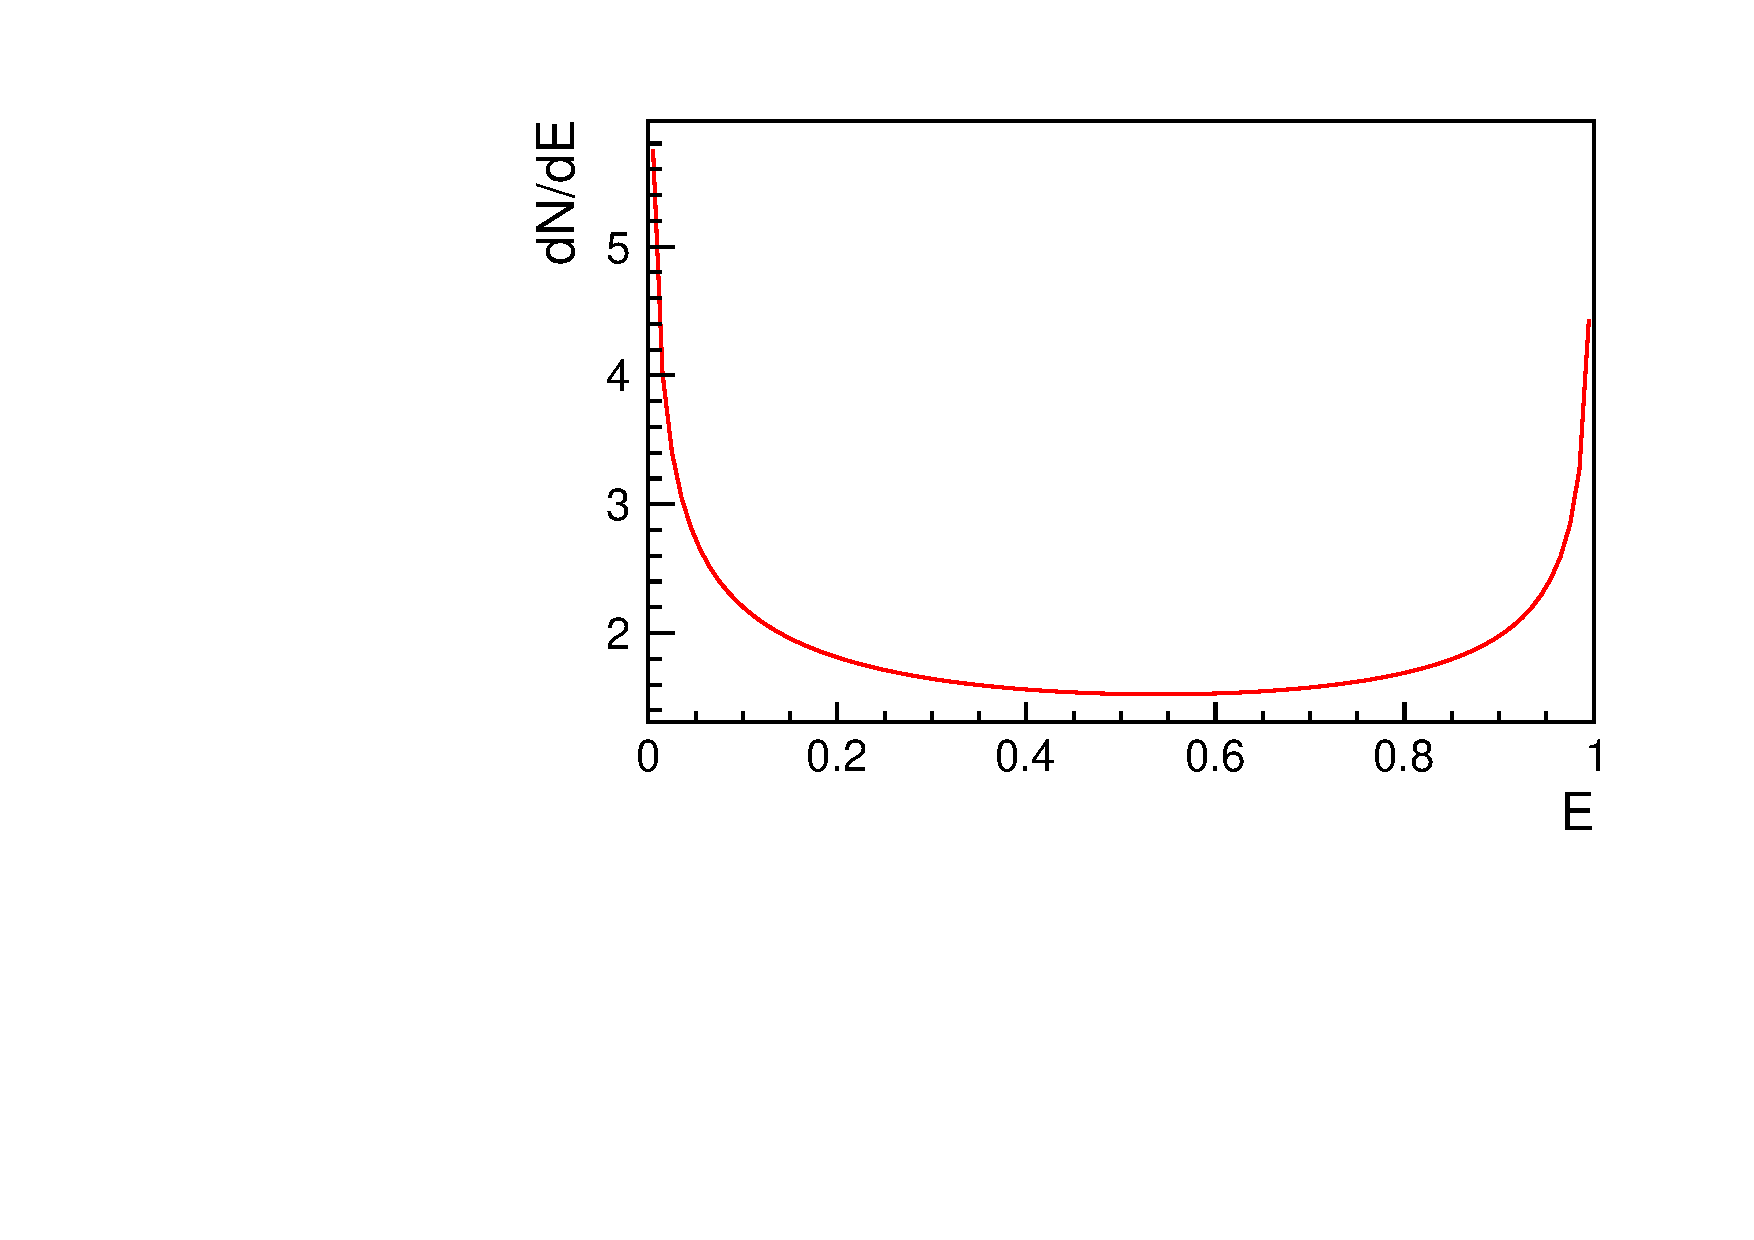
\includegraphics[width=9cm]{BetaFunction_beamspreadpeak.pdf}\\
$a\sim-0.3, b\sim-0.3$
\end{center}
\end{frame}

\begin{frame}
\frametitle{Beta distributions: beam spread in the
arms}\label{slide:betadistspreadarm} 
Beta distribution : $x^a(1-x)^b$ 
\begin{center}
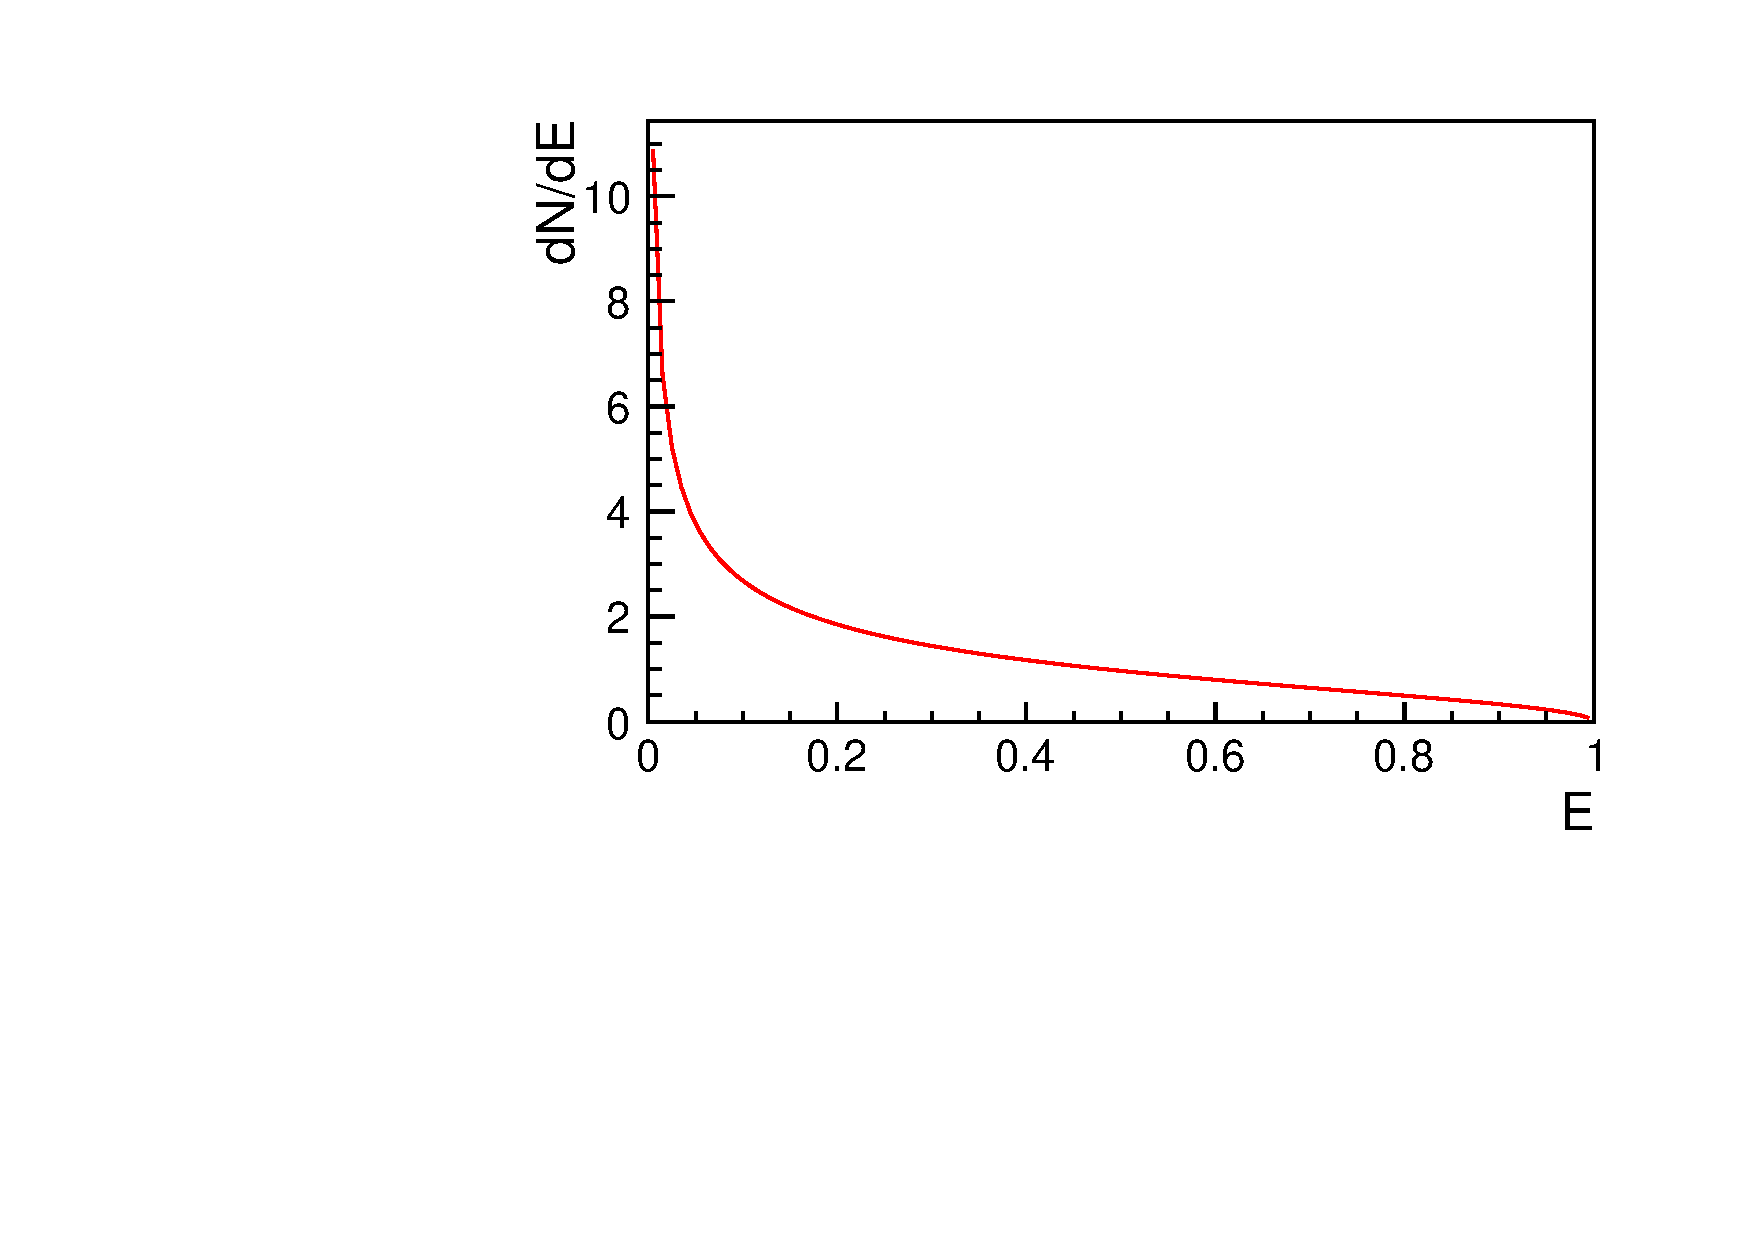
\includegraphics[width=9cm]{BetaFunction_beamspreadarms.pdf}\\
$a\sim-0.4, b\sim0.4$
\end{center}
\end{frame}

\begin{frame}
\frametitle{Model fit results}
\begin{columns}[c]
\column{6cm}
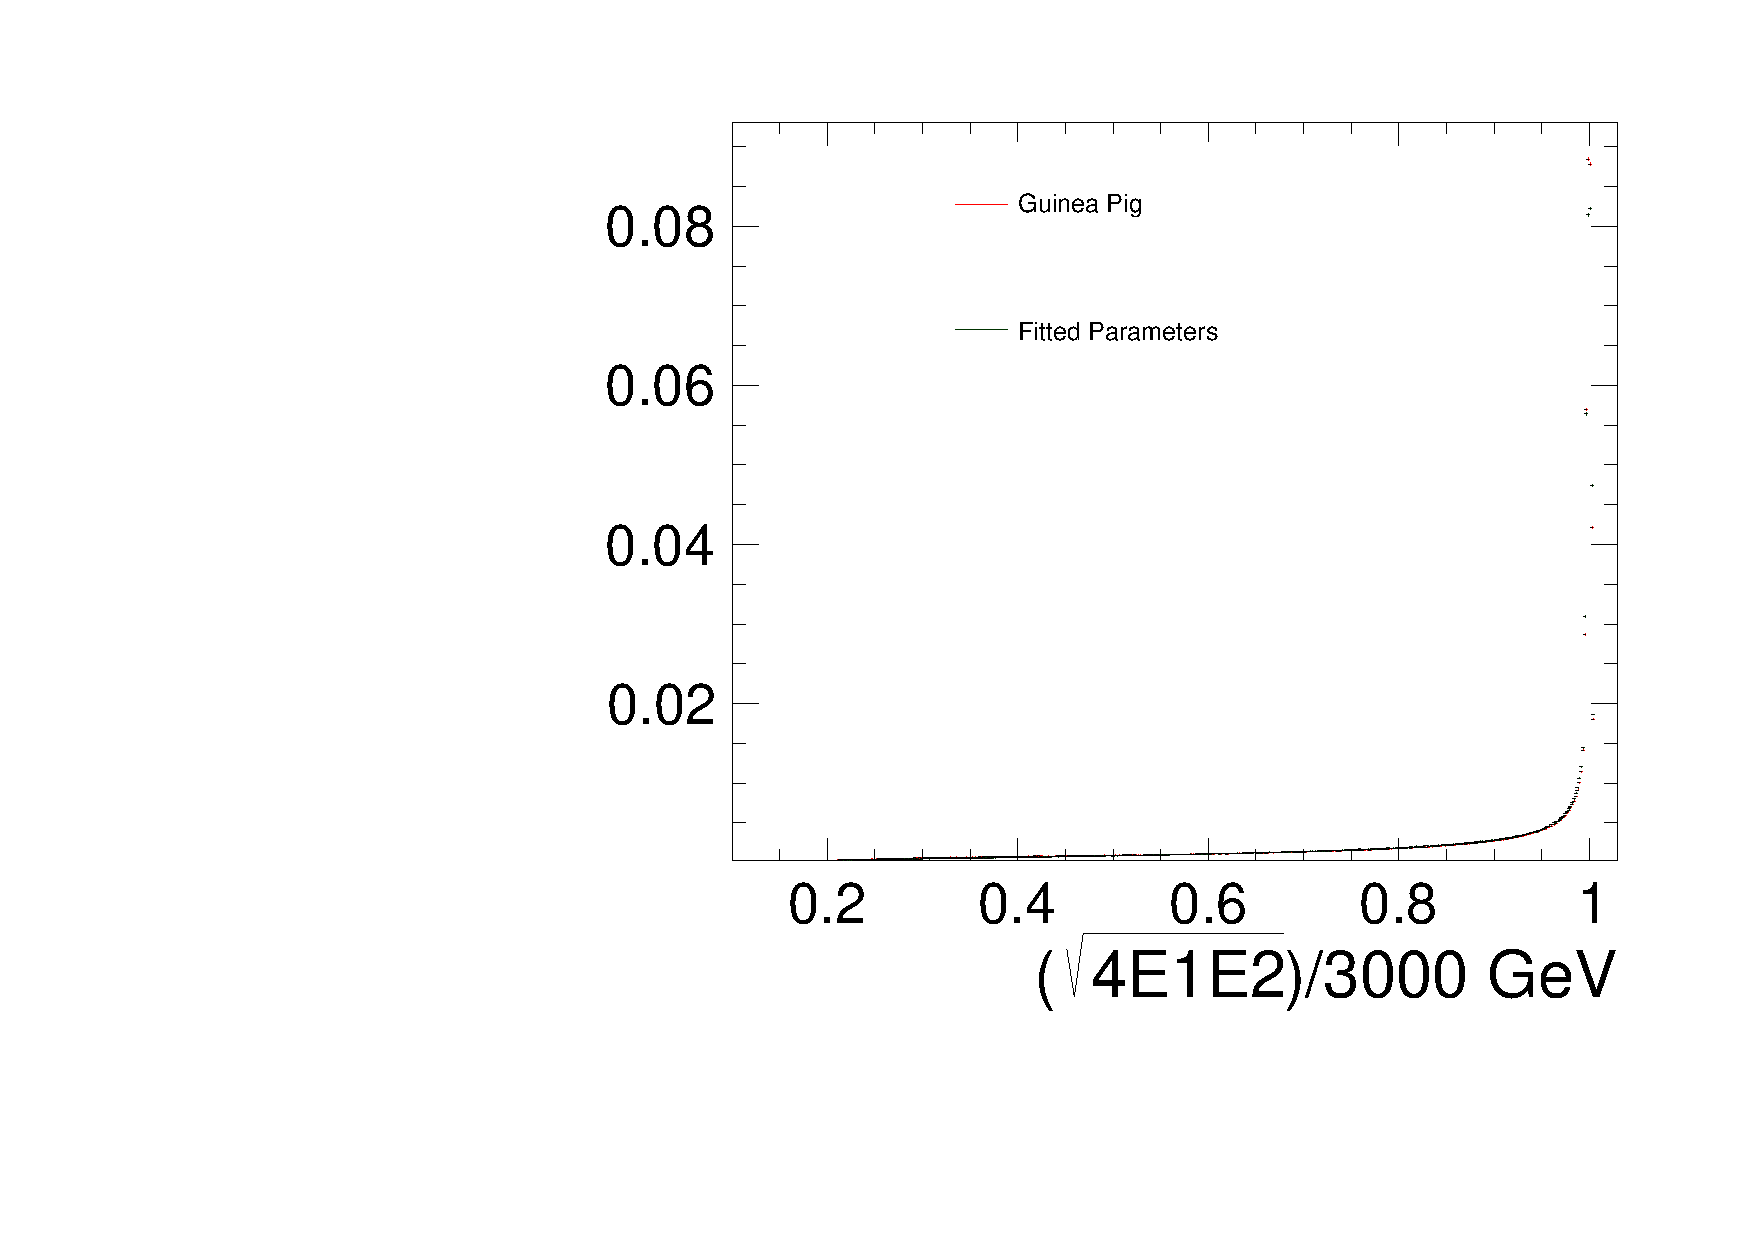
\includegraphics[width=6cm]{FullSpectrumFCAL_notlog.pdf}
\column{6cm}
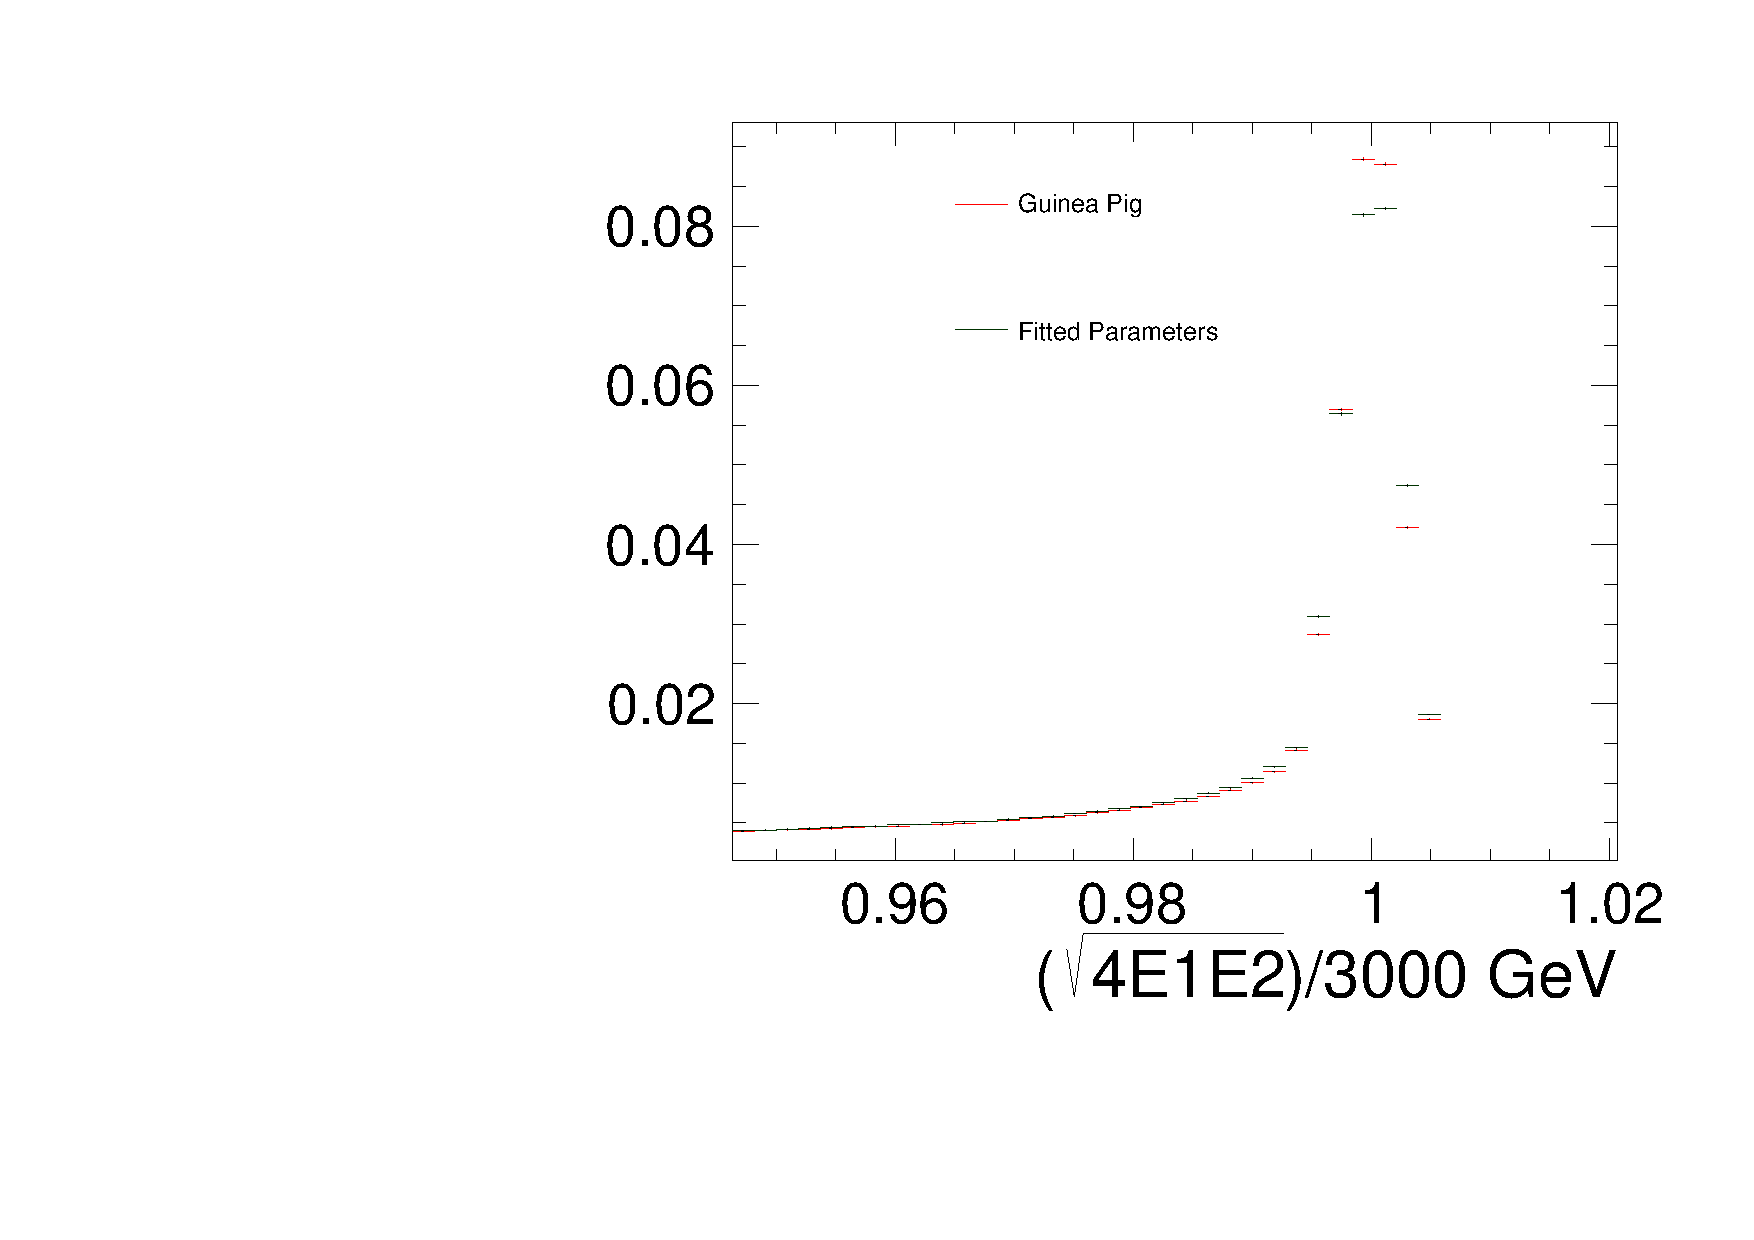
\includegraphics[width=6cm]{FullSpectrumFCAL_zoom_notlog.pdf}
\end{columns}
\end{frame}



\end{document}